\documentclass[twoside]{book}

% Packages required by doxygen
\usepackage{fixltx2e}
\usepackage{calc}
\usepackage{doxygen}
\usepackage[export]{adjustbox} % also loads graphicx
\usepackage{graphicx}
\usepackage[utf8]{inputenc}
\usepackage{makeidx}
\usepackage{multicol}
\usepackage{multirow}
\PassOptionsToPackage{warn}{textcomp}
\usepackage{textcomp}
\usepackage[nointegrals]{wasysym}
\usepackage[table]{xcolor}

% Font selection
\usepackage[T1]{fontenc}
\usepackage[scaled=.90]{helvet}
\usepackage{courier}
\usepackage{amssymb}
\usepackage{sectsty}
\renewcommand{\familydefault}{\sfdefault}
\allsectionsfont{%
  \fontseries{bc}\selectfont%
  \color{darkgray}%
}
\renewcommand{\DoxyLabelFont}{%
  \fontseries{bc}\selectfont%
  \color{darkgray}%
}
\newcommand{\+}{\discretionary{\mbox{\scriptsize$\hookleftarrow$}}{}{}}

% Page & text layout
\usepackage{geometry}
\geometry{%
  a4paper,%
  top=2.5cm,%
  bottom=2.5cm,%
  left=2.5cm,%
  right=2.5cm%
}
\tolerance=750
\hfuzz=15pt
\hbadness=750
\setlength{\emergencystretch}{15pt}
\setlength{\parindent}{0cm}
\setlength{\parskip}{3ex plus 2ex minus 2ex}
\makeatletter
\renewcommand{\paragraph}{%
  \@startsection{paragraph}{4}{0ex}{-1.0ex}{1.0ex}{%
    \normalfont\normalsize\bfseries\SS@parafont%
  }%
}
\renewcommand{\subparagraph}{%
  \@startsection{subparagraph}{5}{0ex}{-1.0ex}{1.0ex}{%
    \normalfont\normalsize\bfseries\SS@subparafont%
  }%
}
\makeatother

% Headers & footers
\usepackage{fancyhdr}
\pagestyle{fancyplain}
\fancyhead[LE]{\fancyplain{}{\bfseries\thepage}}
\fancyhead[CE]{\fancyplain{}{}}
\fancyhead[RE]{\fancyplain{}{\bfseries\leftmark}}
\fancyhead[LO]{\fancyplain{}{\bfseries\rightmark}}
\fancyhead[CO]{\fancyplain{}{}}
\fancyhead[RO]{\fancyplain{}{\bfseries\thepage}}
\fancyfoot[LE]{\fancyplain{}{}}
\fancyfoot[CE]{\fancyplain{}{}}
\fancyfoot[RE]{\fancyplain{}{\bfseries\scriptsize Generated by Doxygen }}
\fancyfoot[LO]{\fancyplain{}{\bfseries\scriptsize Generated by Doxygen }}
\fancyfoot[CO]{\fancyplain{}{}}
\fancyfoot[RO]{\fancyplain{}{}}
\renewcommand{\footrulewidth}{0.4pt}
\renewcommand{\chaptermark}[1]{%
  \markboth{#1}{}%
}
\renewcommand{\sectionmark}[1]{%
  \markright{\thesection\ #1}%
}

% Indices & bibliography
\usepackage{natbib}
\usepackage[titles]{tocloft}
\setcounter{tocdepth}{3}
\setcounter{secnumdepth}{5}
\makeindex

% Hyperlinks (required, but should be loaded last)
\usepackage{ifpdf}
\ifpdf
  \usepackage[pdftex,pagebackref=true]{hyperref}
\else
  \usepackage[ps2pdf,pagebackref=true]{hyperref}
\fi
\hypersetup{%
  colorlinks=true,%
  linkcolor=blue,%
  citecolor=blue,%
  unicode%
}

% Custom commands
\newcommand{\clearemptydoublepage}{%
  \newpage{\pagestyle{empty}\cleardoublepage}%
}

\usepackage{caption}
\captionsetup{labelsep=space,justification=centering,font={bf},singlelinecheck=off,skip=4pt,position=top}

%===== C O N T E N T S =====

\begin{document}

% Titlepage & ToC
\hypersetup{pageanchor=false,
             bookmarksnumbered=true,
             pdfencoding=unicode
            }
\pagenumbering{roman}
\begin{titlepage}
\vspace*{7cm}
\begin{center}%
{\Large E\+E445\+M/\+E\+E380L Lab 5 Documentation }\\
\vspace*{1cm}
{\large Generated by Doxygen 1.8.11}\\
\end{center}
\end{titlepage}
\clearemptydoublepage
\tableofcontents
\clearemptydoublepage
\pagenumbering{arabic}
\hypersetup{pageanchor=true}

%--- Begin generated contents ---
\chapter{Data Structure Index}
\section{Data Structures}
Here are the data structures with brief descriptions\+:\begin{DoxyCompactList}
\item\contentsline{section}{\hyperlink{struct__tcb__s}{\+\_\+tcb\+\_\+s} }{\pageref{struct__tcb__s}}{}
\item\contentsline{section}{\hyperlink{structSema4}{Sema4} }{\pageref{structSema4}}{}
\end{DoxyCompactList}

\chapter{File Index}
\section{File List}
Here is a list of all documented files with brief descriptions\+:\begin{DoxyCompactList}
\item\contentsline{section}{inc/\hyperlink{ADC_8h}{A\+D\+C.\+h} \\*A\+DC driver for the T\+M4\+C123G. Provides interfaces for collecting single samples or a series at a given sampling frequency. Does not allow for sampling of more than one channel at any given time. Timer 2 is reserved for this driver }{\pageref{ADC_8h}}{}
\item\contentsline{section}{inc/{\bfseries asmdefs.\+h} }{\pageref{asmdefs_8h}}{}
\item\contentsline{section}{inc/\hyperlink{diskio_8h}{diskio.\+h} \\*Low level disk interface modlue include file (C)ChaN, 2014 converted to T\+M4\+C123 Jonathan Valvano, January 13, 2015 }{\pageref{diskio_8h}}{}
\item\contentsline{section}{inc/{\bfseries elf.\+h} }{\pageref{elf_8h}}{}
\item\contentsline{section}{inc/\hyperlink{ff_8h}{ff.\+h} \\*Fat\+Fs -\/ F\+AT file system module include file R0.\+10c (C)ChaN, 2014 Fat\+Fs module is a generic F\+AT file system module for small embedded systems. This is a free software that opened for education, research and commercial developments under license policy of following terms. Copyright (C) 2014, , all right reserved. The Fat\+Fs module is a free software and there is NO W\+A\+R\+R\+A\+N\+TY. No restriction on use. You can use, modify and redistribute it for personal, non-\/profit or commercial product U\+N\+D\+ER Y\+O\+UR R\+E\+S\+P\+O\+N\+S\+I\+B\+I\+L\+I\+TY. Redistributions of source code must retain the above copyright notice }{\pageref{ff_8h}}{}
\item\contentsline{section}{inc/{\bfseries ffconf.\+h} }{\pageref{ffconf_8h}}{}
\item\contentsline{section}{inc/{\bfseries F\+I\+F\+O.\+h} }{\pageref{FIFO_8h}}{}
\item\contentsline{section}{inc/\hyperlink{heap_8h}{heap.\+h} \\*Implements memory heap for dynamic memory allocation. Follows standard malloc/calloc/realloc/free interface for allocating/unallocating memory. modified 8/31/08 Jonathan Valvano for style modified 12/16/11 Jonathan Valvano for 32-\/bit machine modified August 10, 2014 for C99 syntax This example accompanies the book \char`\"{}\+Embedded Systems\+: Real Time Operating Systems for A\+R\+M Cortex M Microcontrollers\char`\"{}, I\+S\+BN\+: 978-\/1466468863, Jonathan Valvano, copyright (c) 2014 Implementation Notes\+: This is a Knuth Heap. Each block has a header and a trailer, which I shall call the meta-\/sections. The meta-\/sections are each a single int32\+\_\+t that tells how many int32\+\_\+ts/words can be stored between the header and trailer. If the block is used, the meta-\/sections record the room as a positive number. If the block is unused, the meta-\/sections record the room as a negative number. Copyright 2014 by Jonathan W. Valvano, \href{mailto:valvano@mail.utexas.edu}{\tt valvano@mail.\+utexas.\+edu} You may use, edit, run or distribute this file as long as the above copyright notice remains T\+H\+IS S\+O\+F\+T\+W\+A\+RE IS P\+R\+O\+V\+I\+D\+ED \char`\"{}\+A\+S I\+S\char`\"{}. NO W\+A\+R\+R\+A\+N\+T\+I\+ES, W\+H\+E\+T\+H\+ER E\+X\+P\+R\+E\+SS, I\+M\+P\+L\+I\+ED OR S\+T\+A\+T\+U\+T\+O\+RY, I\+N\+C\+L\+U\+D\+I\+NG, B\+UT N\+OT L\+I\+M\+I\+T\+ED TO, I\+M\+P\+L\+I\+ED W\+A\+R\+R\+A\+N\+T\+I\+ES OF M\+E\+R\+C\+H\+A\+N\+T\+A\+B\+I\+L\+I\+TY A\+ND F\+I\+T\+N\+E\+SS F\+OR A P\+A\+R\+T\+I\+C\+U\+L\+AR P\+U\+R\+P\+O\+SE A\+P\+P\+LY TO T\+H\+IS S\+O\+F\+T\+W\+A\+RE. V\+A\+L\+V\+A\+NO S\+H\+A\+LL N\+OT, IN A\+NY C\+I\+R\+C\+U\+M\+S\+T\+A\+N\+C\+ES, BE L\+I\+A\+B\+LE F\+OR S\+P\+E\+C\+I\+AL, I\+N\+C\+I\+D\+E\+N\+T\+AL, OR C\+O\+N\+S\+E\+Q\+U\+E\+N\+T\+I\+AL D\+A\+M\+A\+G\+ES, F\+OR A\+NY R\+E\+A\+S\+ON W\+H\+A\+T\+S\+O\+E\+V\+ER. For more information about my classes, my research, and my books, see \href{http://users.ece.utexas.edu/~valvano/}{\tt http\+://users.\+ece.\+utexas.\+edu/$\sim$valvano/} }{\pageref{heap_8h}}{}
\item\contentsline{section}{inc/{\bfseries hw\+\_\+adc.\+h} }{\pageref{hw__adc_8h}}{}
\item\contentsline{section}{inc/{\bfseries hw\+\_\+aes.\+h} }{\pageref{hw__aes_8h}}{}
\item\contentsline{section}{inc/{\bfseries hw\+\_\+can.\+h} }{\pageref{hw__can_8h}}{}
\item\contentsline{section}{inc/{\bfseries hw\+\_\+ccm.\+h} }{\pageref{hw__ccm_8h}}{}
\item\contentsline{section}{inc/{\bfseries hw\+\_\+comp.\+h} }{\pageref{hw__comp_8h}}{}
\item\contentsline{section}{inc/{\bfseries hw\+\_\+des.\+h} }{\pageref{hw__des_8h}}{}
\item\contentsline{section}{inc/{\bfseries hw\+\_\+eeprom.\+h} }{\pageref{hw__eeprom_8h}}{}
\item\contentsline{section}{inc/{\bfseries hw\+\_\+emac.\+h} }{\pageref{hw__emac_8h}}{}
\item\contentsline{section}{inc/{\bfseries hw\+\_\+epi.\+h} }{\pageref{hw__epi_8h}}{}
\item\contentsline{section}{inc/{\bfseries hw\+\_\+ethernet.\+h} }{\pageref{hw__ethernet_8h}}{}
\item\contentsline{section}{inc/{\bfseries hw\+\_\+fan.\+h} }{\pageref{hw__fan_8h}}{}
\item\contentsline{section}{inc/{\bfseries hw\+\_\+flash.\+h} }{\pageref{hw__flash_8h}}{}
\item\contentsline{section}{inc/{\bfseries hw\+\_\+gpio.\+h} }{\pageref{hw__gpio_8h}}{}
\item\contentsline{section}{inc/{\bfseries hw\+\_\+hibernate.\+h} }{\pageref{hw__hibernate_8h}}{}
\item\contentsline{section}{inc/{\bfseries hw\+\_\+i2c.\+h} }{\pageref{hw__i2c_8h}}{}
\item\contentsline{section}{inc/{\bfseries hw\+\_\+i2s.\+h} }{\pageref{hw__i2s_8h}}{}
\item\contentsline{section}{inc/{\bfseries hw\+\_\+ints.\+h} }{\pageref{hw__ints_8h}}{}
\item\contentsline{section}{inc/{\bfseries hw\+\_\+lcd.\+h} }{\pageref{hw__lcd_8h}}{}
\item\contentsline{section}{inc/{\bfseries hw\+\_\+lpc.\+h} }{\pageref{hw__lpc_8h}}{}
\item\contentsline{section}{inc/{\bfseries hw\+\_\+memmap.\+h} }{\pageref{hw__memmap_8h}}{}
\item\contentsline{section}{inc/{\bfseries hw\+\_\+nvic.\+h} }{\pageref{hw__nvic_8h}}{}
\item\contentsline{section}{inc/{\bfseries hw\+\_\+peci.\+h} }{\pageref{hw__peci_8h}}{}
\item\contentsline{section}{inc/{\bfseries hw\+\_\+pwm.\+h} }{\pageref{hw__pwm_8h}}{}
\item\contentsline{section}{inc/{\bfseries hw\+\_\+qei.\+h} }{\pageref{hw__qei_8h}}{}
\item\contentsline{section}{inc/{\bfseries hw\+\_\+shamd5.\+h} }{\pageref{hw__shamd5_8h}}{}
\item\contentsline{section}{inc/{\bfseries hw\+\_\+ssi.\+h} }{\pageref{hw__ssi_8h}}{}
\item\contentsline{section}{inc/{\bfseries hw\+\_\+sysctl.\+h} }{\pageref{hw__sysctl_8h}}{}
\item\contentsline{section}{inc/{\bfseries hw\+\_\+sysexc.\+h} }{\pageref{hw__sysexc_8h}}{}
\item\contentsline{section}{inc/{\bfseries hw\+\_\+timer.\+h} }{\pageref{hw__timer_8h}}{}
\item\contentsline{section}{inc/{\bfseries hw\+\_\+types.\+h} }{\pageref{hw__types_8h}}{}
\item\contentsline{section}{inc/{\bfseries hw\+\_\+uart.\+h} }{\pageref{hw__uart_8h}}{}
\item\contentsline{section}{inc/{\bfseries hw\+\_\+udma.\+h} }{\pageref{hw__udma_8h}}{}
\item\contentsline{section}{inc/{\bfseries hw\+\_\+usb.\+h} }{\pageref{hw__usb_8h}}{}
\item\contentsline{section}{inc/{\bfseries hw\+\_\+watchdog.\+h} }{\pageref{hw__watchdog_8h}}{}
\item\contentsline{section}{inc/{\bfseries integer.\+h} }{\pageref{integer_8h}}{}
\item\contentsline{section}{inc/\hyperlink{interpreter_8h}{interpreter.\+h} }{\pageref{interpreter_8h}}{}
\item\contentsline{section}{inc/{\bfseries loader.\+h} }{\pageref{loader_8h}}{}
\item\contentsline{section}{inc/{\bfseries loader\+\_\+config.\+h} }{\pageref{loader__config_8h}}{}
\item\contentsline{section}{inc/\hyperlink{misc__macros_8h}{misc\+\_\+macros.\+h} \\*Some helper macros }{\pageref{misc__macros_8h}}{}
\item\contentsline{section}{inc/\hyperlink{OS_8h}{O\+S.\+h} \\*Real Time Operating System for Labs 2 and 3 E\+E445\+M/\+E\+E380\+L.\+12 }{\pageref{OS_8h}}{}
\item\contentsline{section}{inc/\hyperlink{PLL_8h}{P\+L\+L.\+h} \\*Runs on L\+M4\+F120/\+T\+M4\+C123 A software function to change the bus frequency using the P\+LL }{\pageref{PLL_8h}}{}
\item\contentsline{section}{inc/{\bfseries priorityqueue.\+h} }{\pageref{priorityqueue_8h}}{}
\item\contentsline{section}{inc/\hyperlink{profiler_8h}{profiler.\+h} \\*Thread profiler utility }{\pageref{profiler_8h}}{}
\item\contentsline{section}{inc/\hyperlink{ST7735_8h}{S\+T7735.\+h} \\*Low level drivers for the S\+T7735 }{\pageref{ST7735_8h}}{}
\item\contentsline{section}{inc/\hyperlink{ST7735__lab3_8h}{S\+T7735\+\_\+lab3.\+h} \\*This is a library for the Adafruit 1.\+8" S\+PI display }{\pageref{ST7735__lab3_8h}}{}
\item\contentsline{section}{inc/{\bfseries Switch.\+h} }{\pageref{Switch_8h}}{}
\item\contentsline{section}{inc/{\bfseries time\+Measure.\+h} }{\pageref{timeMeasure_8h}}{}
\item\contentsline{section}{inc/{\bfseries tm4c123gh6pm.\+h} }{\pageref{tm4c123gh6pm_8h}}{}
\item\contentsline{section}{inc/\hyperlink{UART_8h}{U\+A\+R\+T.\+h} \\*Runs on L\+M4\+F120/\+T\+M4\+C123 Use U\+A\+R\+T0 to implement bidirectional data transfer to and from a computer running Hyper\+Terminal. This time, interrupts and F\+I\+F\+Os are used }{\pageref{UART_8h}}{}
\end{DoxyCompactList}

\chapter{Data Structure Documentation}
\hypertarget{struct__tcb__s}{}\section{\+\_\+tcb\+\_\+s Struct Reference}
\label{struct__tcb__s}\index{\+\_\+tcb\+\_\+s@{\+\_\+tcb\+\_\+s}}


Collaboration diagram for \+\_\+tcb\+\_\+s\+:
\nopagebreak
\begin{figure}[H]
\begin{center}
\leavevmode
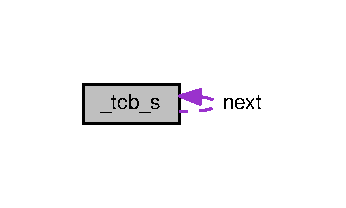
\includegraphics[width=174pt]{struct__tcb__s__coll__graph}
\end{center}
\end{figure}
\subsection*{Data Fields}
\begin{DoxyCompactItemize}
\item 
long $\ast$ {\bfseries sp}\hypertarget{struct__tcb__s_a13f117347df648dbca66e6cbb97a4e0f}{}\label{struct__tcb__s_a13f117347df648dbca66e6cbb97a4e0f}

\item 
struct \hyperlink{struct__tcb__s}{\+\_\+tcb\+\_\+s} $\ast$ {\bfseries next}\hypertarget{struct__tcb__s_af53c260a7b65e7244f809cda9ebb835f}{}\label{struct__tcb__s_af53c260a7b65e7244f809cda9ebb835f}

\item 
uint32\+\_\+t {\bfseries wake\+\_\+time}\hypertarget{struct__tcb__s_a442099ddd859c3f33981828aeef085fe}{}\label{struct__tcb__s_a442099ddd859c3f33981828aeef085fe}

\item 
unsigned long {\bfseries id}\hypertarget{struct__tcb__s_a48e677e5c96cf412d20854802271b9b4}{}\label{struct__tcb__s_a48e677e5c96cf412d20854802271b9b4}

\item 
uint8\+\_\+t {\bfseries priority}\hypertarget{struct__tcb__s_a319151d52db9a3fb0b3c018bce9fcb4a}{}\label{struct__tcb__s_a319151d52db9a3fb0b3c018bce9fcb4a}

\item 
uint32\+\_\+t {\bfseries period}\hypertarget{struct__tcb__s_a85c4e73f3d5ccebf43c628d9e1fc4e4f}{}\label{struct__tcb__s_a85c4e73f3d5ccebf43c628d9e1fc4e4f}

\item 
unsigned long \hyperlink{struct__tcb__s_a1f71cc7a8b23ee420548662caced5301}{magic}\hypertarget{struct__tcb__s_a1f71cc7a8b23ee420548662caced5301}{}\label{struct__tcb__s_a1f71cc7a8b23ee420548662caced5301}

\begin{DoxyCompactList}\small\item\em magic field must contain T\+C\+B\+\_\+\+M\+A\+G\+IC for T\+CB to be valid \end{DoxyCompactList}\item 
void($\ast$ {\bfseries task} )(void)\hypertarget{struct__tcb__s_af815dde5661c4092abe9838fb28d9ed2}{}\label{struct__tcb__s_af815dde5661c4092abe9838fb28d9ed2}

\item 
char $\ast$ {\bfseries task\+\_\+name}\hypertarget{struct__tcb__s_a66241e192445da72f98da4e2d1359d5a}{}\label{struct__tcb__s_a66241e192445da72f98da4e2d1359d5a}

\item 
\hyperlink{struct__pcb__s}{pcb\+\_\+t} $\ast$ {\bfseries parent\+\_\+process}\hypertarget{struct__tcb__s_a95f1ceb9227ec81f5fee8d419e38f6f5}{}\label{struct__tcb__s_a95f1ceb9227ec81f5fee8d419e38f6f5}

\end{DoxyCompactItemize}


The documentation for this struct was generated from the following file\+:\begin{DoxyCompactItemize}
\item 
inc/\hyperlink{OS_8h}{O\+S.\+h}\end{DoxyCompactItemize}

\hypertarget{structDIR}{}\section{D\+IR Struct Reference}
\label{structDIR}\index{D\+IR@{D\+IR}}


Directory object structure (\hyperlink{structDIR}{D\+IR})  




{\ttfamily \#include $<$ff.\+h$>$}



Collaboration diagram for D\+IR\+:\nopagebreak
\begin{figure}[H]
\begin{center}
\leavevmode
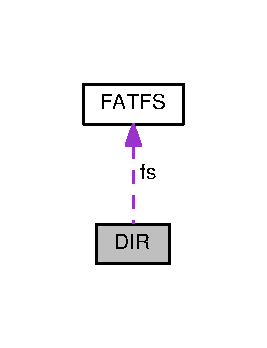
\includegraphics[width=128pt]{structDIR__coll__graph}
\end{center}
\end{figure}
\subsection*{Data Fields}
\begin{DoxyCompactItemize}
\item 
\hyperlink{structFATFS}{F\+A\+T\+FS} $\ast$ {\bfseries fs}\hypertarget{structDIR_a312eaa66cb703fb2993ea98173dc0c9a}{}\label{structDIR_a312eaa66cb703fb2993ea98173dc0c9a}

\item 
W\+O\+RD {\bfseries id}\hypertarget{structDIR_aca2c95a99a04173917ec70c030891383}{}\label{structDIR_aca2c95a99a04173917ec70c030891383}

\item 
W\+O\+RD {\bfseries index}\hypertarget{structDIR_ab95119fbacbe45e3e9ee0f962b844092}{}\label{structDIR_ab95119fbacbe45e3e9ee0f962b844092}

\item 
D\+W\+O\+RD {\bfseries sclust}\hypertarget{structDIR_a9212af5877b94d790dd3bab3aa320994}{}\label{structDIR_a9212af5877b94d790dd3bab3aa320994}

\item 
D\+W\+O\+RD {\bfseries clust}\hypertarget{structDIR_acfbb8ba2d6e73b6f999ceffd1857c190}{}\label{structDIR_acfbb8ba2d6e73b6f999ceffd1857c190}

\item 
D\+W\+O\+RD {\bfseries sect}\hypertarget{structDIR_ad01fcc812ed0dad11a593574336adc9e}{}\label{structDIR_ad01fcc812ed0dad11a593574336adc9e}

\item 
B\+Y\+TE $\ast$ {\bfseries dir}\hypertarget{structDIR_a6c2a8c0cf2d55ae99775e93a16593449}{}\label{structDIR_a6c2a8c0cf2d55ae99775e93a16593449}

\item 
B\+Y\+TE $\ast$ {\bfseries fn}\hypertarget{structDIR_a32da2f31d6c3b6c42eef981cb0cfd2ee}{}\label{structDIR_a32da2f31d6c3b6c42eef981cb0cfd2ee}

\end{DoxyCompactItemize}


\subsection{Detailed Description}
Directory object structure (\hyperlink{structDIR}{D\+IR}) 

The documentation for this struct was generated from the following file\+:\begin{DoxyCompactItemize}
\item 
inc/\hyperlink{ff_8h}{ff.\+h}\end{DoxyCompactItemize}

\hypertarget{structevent__t}{}\section{event\+\_\+t Struct Reference}
\label{structevent__t}\index{event\+\_\+t@{event\+\_\+t}}
\subsection*{Data Fields}
\begin{DoxyCompactItemize}
\item 
event\+\_\+type\+\_\+e {\bfseries type}\hypertarget{structevent__t_a9de80e7379b7765ce1be94f1afdbe299}{}\label{structevent__t_a9de80e7379b7765ce1be94f1afdbe299}

\item 
int {\bfseries magic}\hypertarget{structevent__t_a49228cb7c7840507a14a62231e262ed0}{}\label{structevent__t_a49228cb7c7840507a14a62231e262ed0}

\item 
char $\ast$ {\bfseries name}\hypertarget{structevent__t_a5e267e72cb1799268e9333ed5f05dd85}{}\label{structevent__t_a5e267e72cb1799268e9333ed5f05dd85}

\item 
unsigned long long {\bfseries timestamp}\hypertarget{structevent__t_a0597eb180983129aeddc1033f122b5ce}{}\label{structevent__t_a0597eb180983129aeddc1033f122b5ce}

\end{DoxyCompactItemize}


The documentation for this struct was generated from the following file\+:\begin{DoxyCompactItemize}
\item 
inc/\hyperlink{profiler_8h}{profiler.\+h}\end{DoxyCompactItemize}

\hypertarget{structFATFS}{}\section{F\+A\+T\+FS Struct Reference}
\label{structFATFS}\index{F\+A\+T\+FS@{F\+A\+T\+FS}}


File system object structure (\hyperlink{structFATFS}{F\+A\+T\+FS})  




{\ttfamily \#include $<$ff.\+h$>$}

\subsection*{Data Fields}
\begin{DoxyCompactItemize}
\item 
B\+Y\+TE {\bfseries fs\+\_\+type}\hypertarget{structFATFS_add27d97babe807b573eac98a71dc4ae5}{}\label{structFATFS_add27d97babe807b573eac98a71dc4ae5}

\item 
B\+Y\+TE {\bfseries drv}\hypertarget{structFATFS_a6a791560e2687e8b1569bfce61208d2d}{}\label{structFATFS_a6a791560e2687e8b1569bfce61208d2d}

\item 
B\+Y\+TE {\bfseries csize}\hypertarget{structFATFS_a504a1175f6dcc9a854b9da94463bd108}{}\label{structFATFS_a504a1175f6dcc9a854b9da94463bd108}

\item 
B\+Y\+TE {\bfseries n\+\_\+fats}\hypertarget{structFATFS_a56716c7e7ac10cf46e73ffb2a2e9b545}{}\label{structFATFS_a56716c7e7ac10cf46e73ffb2a2e9b545}

\item 
B\+Y\+TE {\bfseries wflag}\hypertarget{structFATFS_a647e43c9ccae94b7274793d1909897de}{}\label{structFATFS_a647e43c9ccae94b7274793d1909897de}

\item 
B\+Y\+TE {\bfseries fsi\+\_\+flag}\hypertarget{structFATFS_a84e9cdc5a6a8e33ea7ec192058abf161}{}\label{structFATFS_a84e9cdc5a6a8e33ea7ec192058abf161}

\item 
W\+O\+RD {\bfseries id}\hypertarget{structFATFS_a417095d7c20d56d417dc0998e0dd5a5c}{}\label{structFATFS_a417095d7c20d56d417dc0998e0dd5a5c}

\item 
W\+O\+RD {\bfseries n\+\_\+rootdir}\hypertarget{structFATFS_a189a00aa038044ffad0fc7f7dcf2aae1}{}\label{structFATFS_a189a00aa038044ffad0fc7f7dcf2aae1}

\item 
D\+W\+O\+RD {\bfseries last\+\_\+clust}\hypertarget{structFATFS_ad315def289218e26ab78ff90fde700d1}{}\label{structFATFS_ad315def289218e26ab78ff90fde700d1}

\item 
D\+W\+O\+RD {\bfseries free\+\_\+clust}\hypertarget{structFATFS_a5fb49e6ac511bd97eaffdd636d0e4165}{}\label{structFATFS_a5fb49e6ac511bd97eaffdd636d0e4165}

\item 
D\+W\+O\+RD {\bfseries cdir}\hypertarget{structFATFS_a217d0ce0c8cec84aa7f0c142679412c6}{}\label{structFATFS_a217d0ce0c8cec84aa7f0c142679412c6}

\item 
D\+W\+O\+RD {\bfseries n\+\_\+fatent}\hypertarget{structFATFS_a8da50eeba6469bc20d60ca0cf9a1307c}{}\label{structFATFS_a8da50eeba6469bc20d60ca0cf9a1307c}

\item 
D\+W\+O\+RD {\bfseries fsize}\hypertarget{structFATFS_a53e9560659f14e66f306c2c444198bf3}{}\label{structFATFS_a53e9560659f14e66f306c2c444198bf3}

\item 
D\+W\+O\+RD {\bfseries volbase}\hypertarget{structFATFS_a8f0ca578755749d204f59dc83f1a7649}{}\label{structFATFS_a8f0ca578755749d204f59dc83f1a7649}

\item 
D\+W\+O\+RD {\bfseries fatbase}\hypertarget{structFATFS_a848fba02c4aabe02ef2984e578f33d64}{}\label{structFATFS_a848fba02c4aabe02ef2984e578f33d64}

\item 
D\+W\+O\+RD {\bfseries dirbase}\hypertarget{structFATFS_a3f72fd998dbcce4652a85a81fe944bc4}{}\label{structFATFS_a3f72fd998dbcce4652a85a81fe944bc4}

\item 
D\+W\+O\+RD {\bfseries database}\hypertarget{structFATFS_a5b6c0bc2e9fd2ae8ef714210a74a2d5d}{}\label{structFATFS_a5b6c0bc2e9fd2ae8ef714210a74a2d5d}

\item 
D\+W\+O\+RD {\bfseries winsect}\hypertarget{structFATFS_ac60e69c00e6bf7c25febfbac4dc1476b}{}\label{structFATFS_ac60e69c00e6bf7c25febfbac4dc1476b}

\item 
B\+Y\+TE {\bfseries win} \mbox{[}\+\_\+\+M\+A\+X\+\_\+\+SS\mbox{]}\hypertarget{structFATFS_a7cc35a593465e727ab87723c14610644}{}\label{structFATFS_a7cc35a593465e727ab87723c14610644}

\end{DoxyCompactItemize}


\subsection{Detailed Description}
File system object structure (\hyperlink{structFATFS}{F\+A\+T\+FS}) 

The documentation for this struct was generated from the following file\+:\begin{DoxyCompactItemize}
\item 
inc/\hyperlink{ff_8h}{ff.\+h}\end{DoxyCompactItemize}

\hypertarget{structFIL}{}\section{F\+IL Struct Reference}
\label{structFIL}\index{F\+IL@{F\+IL}}


File object structure (\hyperlink{structFIL}{F\+IL})  




{\ttfamily \#include $<$ff.\+h$>$}



Collaboration diagram for F\+IL\+:\nopagebreak
\begin{figure}[H]
\begin{center}
\leavevmode
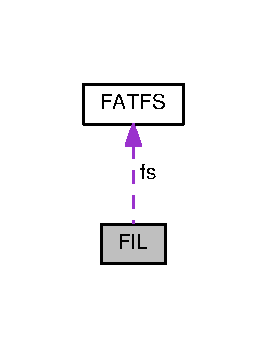
\includegraphics[width=128pt]{structFIL__coll__graph}
\end{center}
\end{figure}
\subsection*{Data Fields}
\begin{DoxyCompactItemize}
\item 
\hyperlink{structFATFS}{F\+A\+T\+FS} $\ast$ {\bfseries fs}\hypertarget{structFIL_a42376a6797a06228911c8b836c1e9030}{}\label{structFIL_a42376a6797a06228911c8b836c1e9030}

\item 
W\+O\+RD {\bfseries id}\hypertarget{structFIL_af7cae0063b0045fb7078b560101ba8f2}{}\label{structFIL_af7cae0063b0045fb7078b560101ba8f2}

\item 
B\+Y\+TE {\bfseries flag}\hypertarget{structFIL_ac409508881f5a16f2998ae675072b376}{}\label{structFIL_ac409508881f5a16f2998ae675072b376}

\item 
B\+Y\+TE {\bfseries err}\hypertarget{structFIL_aea440945db26de9c4a88065c0c887fda}{}\label{structFIL_aea440945db26de9c4a88065c0c887fda}

\item 
D\+W\+O\+RD {\bfseries fptr}\hypertarget{structFIL_a75d29cf9257c827d117887b9f924c4a9}{}\label{structFIL_a75d29cf9257c827d117887b9f924c4a9}

\item 
D\+W\+O\+RD {\bfseries fsize}\hypertarget{structFIL_aa00790d40d7b0081c345fd4f76e22b70}{}\label{structFIL_aa00790d40d7b0081c345fd4f76e22b70}

\item 
D\+W\+O\+RD {\bfseries sclust}\hypertarget{structFIL_ad308b74c8d6975c6a9c30d90b4124c40}{}\label{structFIL_ad308b74c8d6975c6a9c30d90b4124c40}

\item 
D\+W\+O\+RD {\bfseries clust}\hypertarget{structFIL_aa41312aba551b9a6d1c9d3c8c7d2734b}{}\label{structFIL_aa41312aba551b9a6d1c9d3c8c7d2734b}

\item 
D\+W\+O\+RD {\bfseries dsect}\hypertarget{structFIL_ab3d4165d6fd32ac71a130d835fbf0b4d}{}\label{structFIL_ab3d4165d6fd32ac71a130d835fbf0b4d}

\item 
D\+W\+O\+RD {\bfseries dir\+\_\+sect}\hypertarget{structFIL_ab203794f939ad4480e81dfa488770783}{}\label{structFIL_ab203794f939ad4480e81dfa488770783}

\item 
B\+Y\+TE $\ast$ {\bfseries dir\+\_\+ptr}\hypertarget{structFIL_a5af9e9fb312b629220eaf684dd28c4a9}{}\label{structFIL_a5af9e9fb312b629220eaf684dd28c4a9}

\item 
B\+Y\+TE {\bfseries buf} \mbox{[}\+\_\+\+M\+A\+X\+\_\+\+SS\mbox{]}\hypertarget{structFIL_a7a95fb86588663e48309b5cded7e207b}{}\label{structFIL_a7a95fb86588663e48309b5cded7e207b}

\end{DoxyCompactItemize}


\subsection{Detailed Description}
File object structure (\hyperlink{structFIL}{F\+IL}) 

The documentation for this struct was generated from the following file\+:\begin{DoxyCompactItemize}
\item 
inc/\hyperlink{ff_8h}{ff.\+h}\end{DoxyCompactItemize}

\hypertarget{structFILINFO}{}\section{F\+I\+L\+I\+N\+FO Struct Reference}
\label{structFILINFO}\index{F\+I\+L\+I\+N\+FO@{F\+I\+L\+I\+N\+FO}}


File status structure (\hyperlink{structFILINFO}{F\+I\+L\+I\+N\+FO})  




{\ttfamily \#include $<$ff.\+h$>$}

\subsection*{Data Fields}
\begin{DoxyCompactItemize}
\item 
D\+W\+O\+RD {\bfseries fsize}\hypertarget{structFILINFO_aee7441af7dc0c443d1e1e6011cc7dcac}{}\label{structFILINFO_aee7441af7dc0c443d1e1e6011cc7dcac}

\item 
W\+O\+RD {\bfseries fdate}\hypertarget{structFILINFO_a7c01c48a15b1b49da459924437b0bd52}{}\label{structFILINFO_a7c01c48a15b1b49da459924437b0bd52}

\item 
W\+O\+RD {\bfseries ftime}\hypertarget{structFILINFO_ae0f751b79621bf7b29669f177bbe6b9a}{}\label{structFILINFO_ae0f751b79621bf7b29669f177bbe6b9a}

\item 
B\+Y\+TE {\bfseries fattrib}\hypertarget{structFILINFO_a838d542585831b085537b363f18205c0}{}\label{structFILINFO_a838d542585831b085537b363f18205c0}

\item 
T\+C\+H\+AR {\bfseries fname} \mbox{[}13\mbox{]}\hypertarget{structFILINFO_abd852510f2f79b4ec773156d8942dc7c}{}\label{structFILINFO_abd852510f2f79b4ec773156d8942dc7c}

\end{DoxyCompactItemize}


\subsection{Detailed Description}
File status structure (\hyperlink{structFILINFO}{F\+I\+L\+I\+N\+FO}) 

The documentation for this struct was generated from the following file\+:\begin{DoxyCompactItemize}
\item 
inc/\hyperlink{ff_8h}{ff.\+h}\end{DoxyCompactItemize}

\hypertarget{structheap__stats}{}\section{heap\+\_\+stats Struct Reference}
\label{structheap__stats}\index{heap\+\_\+stats@{heap\+\_\+stats}}
\subsection*{Data Fields}
\begin{DoxyCompactItemize}
\item 
int32\+\_\+t {\bfseries words\+Allocated}\hypertarget{structheap__stats_a0399cad6a3b81cc8542f888f9f258bb9}{}\label{structheap__stats_a0399cad6a3b81cc8542f888f9f258bb9}

\item 
int32\+\_\+t {\bfseries words\+Available}\hypertarget{structheap__stats_a284f1c9ea8a59a189cd589815abf5760}{}\label{structheap__stats_a284f1c9ea8a59a189cd589815abf5760}

\item 
int32\+\_\+t {\bfseries words\+Overhead}\hypertarget{structheap__stats_ad2f66b64f88f7e1535ea8b1721c587ef}{}\label{structheap__stats_ad2f66b64f88f7e1535ea8b1721c587ef}

\item 
int32\+\_\+t {\bfseries blocks\+Used}\hypertarget{structheap__stats_a86c4196c97770ce9ab700f1425e5eff1}{}\label{structheap__stats_a86c4196c97770ce9ab700f1425e5eff1}

\item 
int32\+\_\+t {\bfseries blocks\+Unused}\hypertarget{structheap__stats_adc615ee1448dbcbb8ef95e6a42228dbf}{}\label{structheap__stats_adc615ee1448dbcbb8ef95e6a42228dbf}

\end{DoxyCompactItemize}


The documentation for this struct was generated from the following file\+:\begin{DoxyCompactItemize}
\item 
inc/\hyperlink{heap_8h}{heap.\+h}\end{DoxyCompactItemize}

\hypertarget{structSema4}{}\section{Sema4 Struct Reference}
\label{structSema4}\index{Sema4@{Sema4}}


Collaboration diagram for Sema4\+:\nopagebreak
\begin{figure}[H]
\begin{center}
\leavevmode
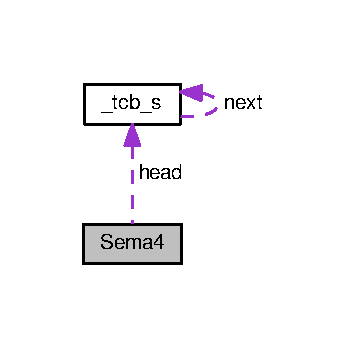
\includegraphics[width=167pt]{structSema4__coll__graph}
\end{center}
\end{figure}
\subsection*{Data Fields}
\begin{DoxyCompactItemize}
\item 
long {\bfseries Value}\hypertarget{structSema4_a98b1e5b4f3a76692bb37db553c22e8b0}{}\label{structSema4_a98b1e5b4f3a76692bb37db553c22e8b0}

\item 
struct \hyperlink{struct__tcb__s}{\+\_\+tcb\+\_\+s} $\ast$ {\bfseries head}\hypertarget{structSema4_a03d774cbfedb9d522f31ded4c10d5668}{}\label{structSema4_a03d774cbfedb9d522f31ded4c10d5668}

\end{DoxyCompactItemize}


The documentation for this struct was generated from the following file\+:\begin{DoxyCompactItemize}
\item 
inc/\hyperlink{OS_8h}{O\+S.\+h}\end{DoxyCompactItemize}

\chapter{File Documentation}
\hypertarget{ADC_8h}{}\section{inc/\+A\+DC.h File Reference}
\label{ADC_8h}\index{inc/\+A\+D\+C.\+h@{inc/\+A\+D\+C.\+h}}


A\+DC driver for the T\+M4\+C123G. Provides interfaces for collecting single samples or a series at a given sampling frequency. Does not allow for sampling of more than one channel at any given time. Timer 2 is reserved for this driver.  


{\ttfamily \#include $<$stdint.\+h$>$}\\*
Include dependency graph for A\+D\+C.\+h\+:\nopagebreak
\begin{figure}[H]
\begin{center}
\leavevmode
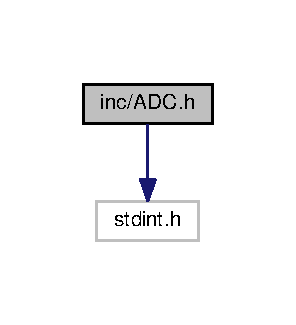
\includegraphics[width=142pt]{ADC_8h__incl}
\end{center}
\end{figure}
\subsection*{Functions}
\begin{DoxyCompactItemize}
\item 
int \hyperlink{ADC_8h_af9d370fc407dee15db32335255f6cf74}{A\+D\+C\+\_\+\+Init} (uint32\+\_\+t channel\+Num)
\begin{DoxyCompactList}\small\item\em Configure an A\+DC channel for continuous sampling. Retrieve measurements from this channel with \hyperlink{ADC_8h_a25269c67b0ba9dd124734e05ffb38493}{A\+D\+C\+\_\+\+In()}. \end{DoxyCompactList}\item 
uint16\+\_\+t \hyperlink{ADC_8h_a25269c67b0ba9dd124734e05ffb38493}{A\+D\+C\+\_\+\+In} (void)
\begin{DoxyCompactList}\small\item\em Returns the most recent sample collected by the channel configured in A\+D\+C\+\_\+\+Init(...) \end{DoxyCompactList}\item 
int \hyperlink{ADC_8h_a262f417393c62f81b4a37b3019b32095}{A\+D\+C\+\_\+\+Collect} (uint32\+\_\+t channel\+Num, uint32\+\_\+t fs, void($\ast$handler)(unsigned long))
\begin{DoxyCompactList}\small\item\em Kick off collection of a sequence of samples to be passed to a user-\/provided handler. The A\+DC and Timer will be configured to collect samples at frequency fs. \end{DoxyCompactList}\end{DoxyCompactItemize}


\subsection{Detailed Description}
A\+DC driver for the T\+M4\+C123G. Provides interfaces for collecting single samples or a series at a given sampling frequency. Does not allow for sampling of more than one channel at any given time. Timer 2 is reserved for this driver. 

\begin{DoxyAuthor}{Author}
Riley Wood and Jeageun Jung 
\end{DoxyAuthor}


\subsection{Function Documentation}
\index{A\+D\+C.\+h@{A\+D\+C.\+h}!A\+D\+C\+\_\+\+Collect@{A\+D\+C\+\_\+\+Collect}}
\index{A\+D\+C\+\_\+\+Collect@{A\+D\+C\+\_\+\+Collect}!A\+D\+C.\+h@{A\+D\+C.\+h}}
\subsubsection[{\texorpdfstring{A\+D\+C\+\_\+\+Collect(uint32\+\_\+t channel\+Num, uint32\+\_\+t fs, void($\ast$handler)(unsigned long))}{ADC_Collect(uint32_t channelNum, uint32_t fs, void(*handler)(unsigned long))}}]{\setlength{\rightskip}{0pt plus 5cm}int A\+D\+C\+\_\+\+Collect (
\begin{DoxyParamCaption}
\item[{uint32\+\_\+t}]{channel\+Num, }
\item[{uint32\+\_\+t}]{fs, }
\item[{void($\ast$)(unsigned long)}]{handler}
\end{DoxyParamCaption}
)}\hypertarget{ADC_8h_a262f417393c62f81b4a37b3019b32095}{}\label{ADC_8h_a262f417393c62f81b4a37b3019b32095}


Kick off collection of a sequence of samples to be passed to a user-\/provided handler. The A\+DC and Timer will be configured to collect samples at frequency fs. 


\begin{DoxyParams}{Parameters}
{\em channel\+Num} & A\+DC channel to sample \\
\hline
{\em fs} & Sampling frequency \\
\hline
{\em handler} & Function which will be passed each sample as it is collected. \\
\hline
\end{DoxyParams}
\begin{DoxyReturn}{Returns}
int 0 on success, -\/1 on failure. 
\end{DoxyReturn}
\index{A\+D\+C.\+h@{A\+D\+C.\+h}!A\+D\+C\+\_\+\+In@{A\+D\+C\+\_\+\+In}}
\index{A\+D\+C\+\_\+\+In@{A\+D\+C\+\_\+\+In}!A\+D\+C.\+h@{A\+D\+C.\+h}}
\subsubsection[{\texorpdfstring{A\+D\+C\+\_\+\+In(void)}{ADC_In(void)}}]{\setlength{\rightskip}{0pt plus 5cm}uint16\+\_\+t A\+D\+C\+\_\+\+In (
\begin{DoxyParamCaption}
\item[{void}]{}
\end{DoxyParamCaption}
)}\hypertarget{ADC_8h_a25269c67b0ba9dd124734e05ffb38493}{}\label{ADC_8h_a25269c67b0ba9dd124734e05ffb38493}


Returns the most recent sample collected by the channel configured in A\+D\+C\+\_\+\+Init(...) 

If the channel has not finished collecting its first sample, this function returns 0x\+F\+F\+FF.

If you call this rapidly, faster than the A\+DC samples, this function may repeat values (since it always returns the most recent).

\begin{DoxyReturn}{Returns}
uint16\+\_\+t The conversion result 
\end{DoxyReturn}
\index{A\+D\+C.\+h@{A\+D\+C.\+h}!A\+D\+C\+\_\+\+Init@{A\+D\+C\+\_\+\+Init}}
\index{A\+D\+C\+\_\+\+Init@{A\+D\+C\+\_\+\+Init}!A\+D\+C.\+h@{A\+D\+C.\+h}}
\subsubsection[{\texorpdfstring{A\+D\+C\+\_\+\+Init(uint32\+\_\+t channel\+Num)}{ADC_Init(uint32_t channelNum)}}]{\setlength{\rightskip}{0pt plus 5cm}int A\+D\+C\+\_\+\+Init (
\begin{DoxyParamCaption}
\item[{uint32\+\_\+t}]{channel\+Num}
\end{DoxyParamCaption}
)}\hypertarget{ADC_8h_af9d370fc407dee15db32335255f6cf74}{}\label{ADC_8h_af9d370fc407dee15db32335255f6cf74}


Configure an A\+DC channel for continuous sampling. Retrieve measurements from this channel with \hyperlink{ADC_8h_a25269c67b0ba9dd124734e05ffb38493}{A\+D\+C\+\_\+\+In()}. 


\begin{DoxyParams}{Parameters}
{\em channel\+Num} & The channel to set up \\
\hline
\end{DoxyParams}
\begin{DoxyReturn}{Returns}
int 0 on success, -\/1 on failure. 
\end{DoxyReturn}

\hypertarget{diskio_8h}{}\section{inc/diskio.h File Reference}
\label{diskio_8h}\index{inc/diskio.\+h@{inc/diskio.\+h}}


Low level disk interface modlue include file (C)ChaN, 2014 converted to T\+M4\+C123 Jonathan Valvano, January 13, 2015.  


{\ttfamily \#include \char`\"{}integer.\+h\char`\"{}}\\*
Include dependency graph for diskio.\+h\+:\nopagebreak
\begin{figure}[H]
\begin{center}
\leavevmode
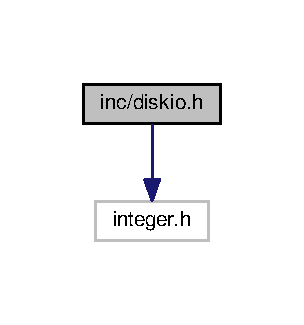
\includegraphics[width=146pt]{diskio_8h__incl}
\end{center}
\end{figure}
\subsection*{Macros}
\begin{DoxyCompactItemize}
\item 
\#define {\bfseries \+\_\+\+U\+S\+E\+\_\+\+W\+R\+I\+TE}~1  /$\ast$ 1\+: Enable \hyperlink{diskio_8h_ac03220b2c8a090b4f76eb2c9407b84fb}{disk\+\_\+write}() function $\ast$/\hypertarget{diskio_8h_a1dd0d2b46dce637878416d489d2ddde2}{}\label{diskio_8h_a1dd0d2b46dce637878416d489d2ddde2}

\item 
\#define {\bfseries \+\_\+\+U\+S\+E\+\_\+\+I\+O\+C\+TL}~1  /$\ast$ 1\+: Enable \hyperlink{diskio_8h_ac822cf3c1768a2c35e4858cc99b8f53b}{disk\+\_\+ioctl}() fucntion $\ast$/\hypertarget{diskio_8h_afe6d1224687dede333375a2475c78ff6}{}\label{diskio_8h_afe6d1224687dede333375a2475c78ff6}

\item 
\#define {\bfseries S\+T\+A\+\_\+\+N\+O\+I\+N\+IT}~0x01  /$\ast$ Drive not initialized $\ast$/\hypertarget{diskio_8h_abd6503c70d862b979a3f7080a59e9acd}{}\label{diskio_8h_abd6503c70d862b979a3f7080a59e9acd}

\item 
\#define {\bfseries S\+T\+A\+\_\+\+N\+O\+D\+I\+SK}~0x02  /$\ast$ No medium in the drive $\ast$/\hypertarget{diskio_8h_aec625080763d6cf487e550a6c9a2dd19}{}\label{diskio_8h_aec625080763d6cf487e550a6c9a2dd19}

\item 
\#define {\bfseries S\+T\+A\+\_\+\+P\+R\+O\+T\+E\+CT}~0x04  /$\ast$ Write protected $\ast$/\hypertarget{diskio_8h_a9ec6dc5f6620a33fabe388d3a111ca8c}{}\label{diskio_8h_a9ec6dc5f6620a33fabe388d3a111ca8c}

\item 
\#define {\bfseries C\+T\+R\+L\+\_\+\+S\+Y\+NC}~0  /$\ast$ Complete pending write process (needed at \+\_\+\+F\+S\+\_\+\+R\+E\+A\+D\+O\+N\+LY == 0) $\ast$/\hypertarget{diskio_8h_a1b3c492f9aec325f0655941b75256f3c}{}\label{diskio_8h_a1b3c492f9aec325f0655941b75256f3c}

\item 
\#define {\bfseries G\+E\+T\+\_\+\+S\+E\+C\+T\+O\+R\+\_\+\+C\+O\+U\+NT}~1  /$\ast$ Get media size (needed at \+\_\+\+U\+S\+E\+\_\+\+M\+K\+FS == 1) $\ast$/\hypertarget{diskio_8h_a570216006f6a8fc4e1698b1bbb2d1dde}{}\label{diskio_8h_a570216006f6a8fc4e1698b1bbb2d1dde}

\item 
\#define {\bfseries G\+E\+T\+\_\+\+S\+E\+C\+T\+O\+R\+\_\+\+S\+I\+ZE}~2  /$\ast$ Get sector size (needed at \+\_\+\+M\+A\+X\+\_\+\+SS != \+\_\+\+M\+I\+N\+\_\+\+SS) $\ast$/\hypertarget{diskio_8h_ac73b5cf2135cbd459d109b96c9aa346a}{}\label{diskio_8h_ac73b5cf2135cbd459d109b96c9aa346a}

\item 
\#define {\bfseries G\+E\+T\+\_\+\+B\+L\+O\+C\+K\+\_\+\+S\+I\+ZE}~3  /$\ast$ Get erase block size (needed at \+\_\+\+U\+S\+E\+\_\+\+M\+K\+FS == 1) $\ast$/\hypertarget{diskio_8h_aec3bb4dfe075d0ba2f3b07b300a95500}{}\label{diskio_8h_aec3bb4dfe075d0ba2f3b07b300a95500}

\item 
\#define {\bfseries C\+T\+R\+L\+\_\+\+T\+R\+IM}~4  /$\ast$ Inform device that the data on the block of sectors is no longer used (needed at \+\_\+\+U\+S\+E\+\_\+\+T\+R\+IM == 1) $\ast$/\hypertarget{diskio_8h_af09fd84bea8d4e889e272471f44d60d6}{}\label{diskio_8h_af09fd84bea8d4e889e272471f44d60d6}

\item 
\#define {\bfseries C\+T\+R\+L\+\_\+\+F\+O\+R\+M\+AT}~5  /$\ast$ Create physical format on the media $\ast$/\hypertarget{diskio_8h_add07021167069f5914211a2f8830fabb}{}\label{diskio_8h_add07021167069f5914211a2f8830fabb}

\item 
\#define {\bfseries C\+T\+R\+L\+\_\+\+P\+O\+W\+E\+R\+\_\+\+I\+D\+LE}~6  /$\ast$ Put the device idle state $\ast$/\hypertarget{diskio_8h_a69bec9079062f809c3586977b2dc5d79}{}\label{diskio_8h_a69bec9079062f809c3586977b2dc5d79}

\item 
\#define {\bfseries C\+T\+R\+L\+\_\+\+P\+O\+W\+E\+R\+\_\+\+O\+FF}~7  /$\ast$ Put the device off state $\ast$/\hypertarget{diskio_8h_aa1f5a55ea2a24d274c16e51c111c97d8}{}\label{diskio_8h_aa1f5a55ea2a24d274c16e51c111c97d8}

\item 
\#define {\bfseries C\+T\+R\+L\+\_\+\+L\+O\+CK}~8  /$\ast$ Lock media removal $\ast$/\hypertarget{diskio_8h_af40e5cf3000553a978ff6e30dae70858}{}\label{diskio_8h_af40e5cf3000553a978ff6e30dae70858}

\item 
\#define {\bfseries C\+T\+R\+L\+\_\+\+U\+N\+L\+O\+CK}~9  /$\ast$ Unlock media removal $\ast$/\hypertarget{diskio_8h_a5d06770de580667138ca6101ae5138ac}{}\label{diskio_8h_a5d06770de580667138ca6101ae5138ac}

\item 
\#define {\bfseries C\+T\+R\+L\+\_\+\+E\+J\+E\+CT}~10  /$\ast$ Eject media $\ast$/\hypertarget{diskio_8h_a5e40e16d2d7ce196858950f070b9ec03}{}\label{diskio_8h_a5e40e16d2d7ce196858950f070b9ec03}

\item 
\#define {\bfseries M\+M\+C\+\_\+\+G\+E\+T\+\_\+\+T\+Y\+PE}~50  /$\ast$ Get card type $\ast$/\hypertarget{diskio_8h_aba3a81a9a47c7d1bf3ac7749bc72dcfd}{}\label{diskio_8h_aba3a81a9a47c7d1bf3ac7749bc72dcfd}

\item 
\#define {\bfseries M\+M\+C\+\_\+\+G\+E\+T\+\_\+\+C\+SD}~51  /$\ast$ Get C\+SD $\ast$/\hypertarget{diskio_8h_ae3b858b81287929f7c7bea3b7aec3087}{}\label{diskio_8h_ae3b858b81287929f7c7bea3b7aec3087}

\item 
\#define {\bfseries M\+M\+C\+\_\+\+G\+E\+T\+\_\+\+C\+ID}~52  /$\ast$ Get C\+ID $\ast$/\hypertarget{diskio_8h_a17ad303dd18b19a4c90ab30a8a1c14c4}{}\label{diskio_8h_a17ad303dd18b19a4c90ab30a8a1c14c4}

\item 
\#define {\bfseries M\+M\+C\+\_\+\+G\+E\+T\+\_\+\+O\+CR}~53  /$\ast$ Get O\+CR $\ast$/\hypertarget{diskio_8h_aff118ba6bd7a9fe7699cee049cff5d6c}{}\label{diskio_8h_aff118ba6bd7a9fe7699cee049cff5d6c}

\item 
\#define {\bfseries M\+M\+C\+\_\+\+G\+E\+T\+\_\+\+S\+D\+S\+T\+AT}~54  /$\ast$ Get SD status $\ast$/\hypertarget{diskio_8h_a5cc43c8449b872e16ea5ab42592f793e}{}\label{diskio_8h_a5cc43c8449b872e16ea5ab42592f793e}

\item 
\#define {\bfseries A\+T\+A\+\_\+\+G\+E\+T\+\_\+\+R\+EV}~60  /$\ast$ Get F/W revision $\ast$/\hypertarget{diskio_8h_a23f5fff3341e98825ea1f7367fd09f1a}{}\label{diskio_8h_a23f5fff3341e98825ea1f7367fd09f1a}

\item 
\#define {\bfseries A\+T\+A\+\_\+\+G\+E\+T\+\_\+\+M\+O\+D\+EL}~61  /$\ast$ Get model name $\ast$/\hypertarget{diskio_8h_a31f556ab98ab80c39058b38d9283865d}{}\label{diskio_8h_a31f556ab98ab80c39058b38d9283865d}

\item 
\#define {\bfseries A\+T\+A\+\_\+\+G\+E\+T\+\_\+\+SN}~62  /$\ast$ Get serial number $\ast$/\hypertarget{diskio_8h_a469c4f989757ee1ee404134fea3c74ba}{}\label{diskio_8h_a469c4f989757ee1ee404134fea3c74ba}

\item 
\#define {\bfseries C\+T\+\_\+\+M\+MC}~0x01    /$\ast$ M\+M\+C ver 3 $\ast$/\hypertarget{diskio_8h_ac52ec66c278308382fdf7b2c57f0ad8c}{}\label{diskio_8h_ac52ec66c278308382fdf7b2c57f0ad8c}

\item 
\#define {\bfseries C\+T\+\_\+\+S\+D1}~0x02    /$\ast$ S\+D ver 1 $\ast$/\hypertarget{diskio_8h_ad1c9fc863ec15d3320b3850dc571626e}{}\label{diskio_8h_ad1c9fc863ec15d3320b3850dc571626e}

\item 
\#define {\bfseries C\+T\+\_\+\+S\+D2}~0x04    /$\ast$ S\+D ver 2 $\ast$/\hypertarget{diskio_8h_a0db1b71113e73184a5ba511e7020a922}{}\label{diskio_8h_a0db1b71113e73184a5ba511e7020a922}

\item 
\#define {\bfseries C\+T\+\_\+\+S\+DC}~(C\+T\+\_\+\+S\+D1$\vert$C\+T\+\_\+\+S\+D2)  /$\ast$ SD $\ast$/\hypertarget{diskio_8h_ae76d94ac83c68d1f025cb0bcad77fa5d}{}\label{diskio_8h_ae76d94ac83c68d1f025cb0bcad77fa5d}

\item 
\#define {\bfseries C\+T\+\_\+\+B\+L\+O\+CK}~0x08    /$\ast$ Block addressing $\ast$/\hypertarget{diskio_8h_a7d48ce54c27f4f60666309e8627fab47}{}\label{diskio_8h_a7d48ce54c27f4f60666309e8627fab47}

\end{DoxyCompactItemize}
\subsection*{Typedefs}
\begin{DoxyCompactItemize}
\item 
typedef B\+Y\+TE \hyperlink{diskio_8h_adba6790898ce4029c20a34b898ce73c1}{D\+S\+T\+A\+T\+US}\hypertarget{diskio_8h_adba6790898ce4029c20a34b898ce73c1}{}\label{diskio_8h_adba6790898ce4029c20a34b898ce73c1}

\begin{DoxyCompactList}\small\item\em Status of Disk Functions. \end{DoxyCompactList}\end{DoxyCompactItemize}
\subsection*{Enumerations}
\begin{DoxyCompactItemize}
\item 
enum \hyperlink{diskio_8h_aacdfef1dad6565f65c26d12fe0ea4b2b}{D\+R\+E\+S\+U\+LT} \{ \\*
{\bfseries R\+E\+S\+\_\+\+OK} = 0, 
{\bfseries R\+E\+S\+\_\+\+E\+R\+R\+OR}, 
{\bfseries R\+E\+S\+\_\+\+W\+R\+P\+RT}, 
{\bfseries R\+E\+S\+\_\+\+N\+O\+T\+R\+DY}, 
\\*
{\bfseries R\+E\+S\+\_\+\+P\+A\+R\+E\+RR}
 \}\hypertarget{diskio_8h_aacdfef1dad6565f65c26d12fe0ea4b2b}{}\label{diskio_8h_aacdfef1dad6565f65c26d12fe0ea4b2b}
\begin{DoxyCompactList}\small\item\em Results of Disk Functions. \end{DoxyCompactList}
\end{DoxyCompactItemize}
\subsection*{Functions}
\begin{DoxyCompactItemize}
\item 
\hyperlink{diskio_8h_adba6790898ce4029c20a34b898ce73c1}{D\+S\+T\+A\+T\+US} \hyperlink{diskio_8h_a8e429a29bdbb73f5bc9e2ab2335a5112}{disk\+\_\+initialize} (B\+Y\+TE drv)
\begin{DoxyCompactList}\small\item\em Initialize disk drive. \end{DoxyCompactList}\item 
\hyperlink{diskio_8h_adba6790898ce4029c20a34b898ce73c1}{D\+S\+T\+A\+T\+US} \hyperlink{diskio_8h_a21ad8e9a107ea2000705a3edfebaaa2d}{disk\+\_\+status} (B\+Y\+TE drv)
\begin{DoxyCompactList}\small\item\em Get disk status. \end{DoxyCompactList}\item 
\hyperlink{diskio_8h_aacdfef1dad6565f65c26d12fe0ea4b2b}{D\+R\+E\+S\+U\+LT} \hyperlink{diskio_8h_a99e229031022d13ac273b6ea78af49cd}{disk\+\_\+read} (B\+Y\+TE drv, B\+Y\+TE $\ast$buff, D\+W\+O\+RD sector, U\+I\+NT count)
\begin{DoxyCompactList}\small\item\em Read sector(s) \end{DoxyCompactList}\item 
\hyperlink{diskio_8h_aacdfef1dad6565f65c26d12fe0ea4b2b}{D\+R\+E\+S\+U\+LT} \hyperlink{diskio_8h_ac03220b2c8a090b4f76eb2c9407b84fb}{disk\+\_\+write} (B\+Y\+TE drv, const B\+Y\+TE $\ast$buff, D\+W\+O\+RD sector, U\+I\+NT count)
\begin{DoxyCompactList}\small\item\em Write sector(s) \end{DoxyCompactList}\item 
\hyperlink{diskio_8h_aacdfef1dad6565f65c26d12fe0ea4b2b}{D\+R\+E\+S\+U\+LT} \hyperlink{diskio_8h_ac822cf3c1768a2c35e4858cc99b8f53b}{disk\+\_\+ioctl} (B\+Y\+TE drv, B\+Y\+TE cmd, void $\ast$buff)
\begin{DoxyCompactList}\small\item\em Miscellaneous drive controls. \end{DoxyCompactList}\end{DoxyCompactItemize}


\subsection{Detailed Description}
Low level disk interface modlue include file (C)ChaN, 2014 converted to T\+M4\+C123 Jonathan Valvano, January 13, 2015. 



\subsection{Function Documentation}
\index{diskio.\+h@{diskio.\+h}!disk\+\_\+initialize@{disk\+\_\+initialize}}
\index{disk\+\_\+initialize@{disk\+\_\+initialize}!diskio.\+h@{diskio.\+h}}
\subsubsection[{\texorpdfstring{disk\+\_\+initialize(\+B\+Y\+T\+E drv)}{disk_initialize(BYTE drv)}}]{\setlength{\rightskip}{0pt plus 5cm}{\bf D\+S\+T\+A\+T\+US} disk\+\_\+initialize (
\begin{DoxyParamCaption}
\item[{B\+Y\+TE}]{drv}
\end{DoxyParamCaption}
)}\hypertarget{diskio_8h_a8e429a29bdbb73f5bc9e2ab2335a5112}{}\label{diskio_8h_a8e429a29bdbb73f5bc9e2ab2335a5112}


Initialize disk drive. 


\begin{DoxyParams}{Parameters}
{\em drv} & Physical drive number, which must be 0 \\
\hline
\end{DoxyParams}
\begin{DoxyReturn}{Returns}
status (see D\+S\+T\+A\+T\+US) 
\end{DoxyReturn}
\index{diskio.\+h@{diskio.\+h}!disk\+\_\+ioctl@{disk\+\_\+ioctl}}
\index{disk\+\_\+ioctl@{disk\+\_\+ioctl}!diskio.\+h@{diskio.\+h}}
\subsubsection[{\texorpdfstring{disk\+\_\+ioctl(\+B\+Y\+T\+E drv, B\+Y\+T\+E cmd, void $\ast$buff)}{disk_ioctl(BYTE drv, BYTE cmd, void *buff)}}]{\setlength{\rightskip}{0pt plus 5cm}{\bf D\+R\+E\+S\+U\+LT} disk\+\_\+ioctl (
\begin{DoxyParamCaption}
\item[{B\+Y\+TE}]{drv, }
\item[{B\+Y\+TE}]{cmd, }
\item[{void $\ast$}]{buff}
\end{DoxyParamCaption}
)}\hypertarget{diskio_8h_ac822cf3c1768a2c35e4858cc99b8f53b}{}\label{diskio_8h_ac822cf3c1768a2c35e4858cc99b8f53b}


Miscellaneous drive controls. 


\begin{DoxyParams}{Parameters}
{\em drv} & Physical drive number (0) \\
\hline
{\em cmd} & Control command code \\
\hline
{\em buff} & Pointer to the control data \\
\hline
\end{DoxyParams}
\begin{DoxyReturn}{Returns}
status (see D\+R\+E\+S\+U\+LT) 
\end{DoxyReturn}
\index{diskio.\+h@{diskio.\+h}!disk\+\_\+read@{disk\+\_\+read}}
\index{disk\+\_\+read@{disk\+\_\+read}!diskio.\+h@{diskio.\+h}}
\subsubsection[{\texorpdfstring{disk\+\_\+read(\+B\+Y\+T\+E drv, B\+Y\+T\+E $\ast$buff, D\+W\+O\+R\+D sector, U\+I\+N\+T count)}{disk_read(BYTE drv, BYTE *buff, DWORD sector, UINT count)}}]{\setlength{\rightskip}{0pt plus 5cm}{\bf D\+R\+E\+S\+U\+LT} disk\+\_\+read (
\begin{DoxyParamCaption}
\item[{B\+Y\+TE}]{drv, }
\item[{B\+Y\+TE $\ast$}]{buff, }
\item[{D\+W\+O\+RD}]{sector, }
\item[{U\+I\+NT}]{count}
\end{DoxyParamCaption}
)}\hypertarget{diskio_8h_a99e229031022d13ac273b6ea78af49cd}{}\label{diskio_8h_a99e229031022d13ac273b6ea78af49cd}


Read sector(s) 


\begin{DoxyParams}{Parameters}
{\em drv} & Physical drive number (0) \\
\hline
{\em buff} & Pointer to the data buffer to store read data \\
\hline
{\em sector} & Start sector number (L\+BA) \\
\hline
{\em count} & Number of sectors to read (1..128) \\
\hline
\end{DoxyParams}
\begin{DoxyReturn}{Returns}
status (see D\+R\+E\+S\+U\+LT) 
\end{DoxyReturn}
\index{diskio.\+h@{diskio.\+h}!disk\+\_\+status@{disk\+\_\+status}}
\index{disk\+\_\+status@{disk\+\_\+status}!diskio.\+h@{diskio.\+h}}
\subsubsection[{\texorpdfstring{disk\+\_\+status(\+B\+Y\+T\+E drv)}{disk_status(BYTE drv)}}]{\setlength{\rightskip}{0pt plus 5cm}{\bf D\+S\+T\+A\+T\+US} disk\+\_\+status (
\begin{DoxyParamCaption}
\item[{B\+Y\+TE}]{drv}
\end{DoxyParamCaption}
)}\hypertarget{diskio_8h_a21ad8e9a107ea2000705a3edfebaaa2d}{}\label{diskio_8h_a21ad8e9a107ea2000705a3edfebaaa2d}


Get disk status. 


\begin{DoxyParams}{Parameters}
{\em drv} & Physical drive number, which must be 0 \\
\hline
\end{DoxyParams}
\begin{DoxyReturn}{Returns}
status (see D\+S\+T\+A\+T\+US) 
\end{DoxyReturn}
\index{diskio.\+h@{diskio.\+h}!disk\+\_\+write@{disk\+\_\+write}}
\index{disk\+\_\+write@{disk\+\_\+write}!diskio.\+h@{diskio.\+h}}
\subsubsection[{\texorpdfstring{disk\+\_\+write(\+B\+Y\+T\+E drv, const B\+Y\+T\+E $\ast$buff, D\+W\+O\+R\+D sector, U\+I\+N\+T count)}{disk_write(BYTE drv, const BYTE *buff, DWORD sector, UINT count)}}]{\setlength{\rightskip}{0pt plus 5cm}{\bf D\+R\+E\+S\+U\+LT} disk\+\_\+write (
\begin{DoxyParamCaption}
\item[{B\+Y\+TE}]{drv, }
\item[{const B\+Y\+TE $\ast$}]{buff, }
\item[{D\+W\+O\+RD}]{sector, }
\item[{U\+I\+NT}]{count}
\end{DoxyParamCaption}
)}\hypertarget{diskio_8h_ac03220b2c8a090b4f76eb2c9407b84fb}{}\label{diskio_8h_ac03220b2c8a090b4f76eb2c9407b84fb}


Write sector(s) 


\begin{DoxyParams}{Parameters}
{\em drv} & Physical drive number (0) \\
\hline
{\em buff} & Pointer to the data buffer to write to disk \\
\hline
{\em sector} & Start sector number (L\+BA) \\
\hline
{\em count} & Number of sectors to write (1..128) \\
\hline
\end{DoxyParams}
\begin{DoxyReturn}{Returns}
status (see D\+R\+E\+S\+U\+LT) 
\end{DoxyReturn}

\hypertarget{ff_8h}{}\section{inc/ff.h File Reference}
\label{ff_8h}\index{inc/ff.\+h@{inc/ff.\+h}}


Fat\+Fs -\/ F\+AT file system module include file R0.\+10c (C)ChaN, 2014 Fat\+Fs module is a generic F\+AT file system module for small embedded systems. This is a free software that opened for education, research and commercial developments under license policy of following terms. Copyright (C) 2014, , all right reserved. The Fat\+Fs module is a free software and there is NO W\+A\+R\+R\+A\+N\+TY. No restriction on use. You can use, modify and redistribute it for personal, non-\/profit or commercial product U\+N\+D\+ER Y\+O\+UR R\+E\+S\+P\+O\+N\+S\+I\+B\+I\+L\+I\+TY. Redistributions of source code must retain the above copyright notice.  


{\ttfamily \#include \char`\"{}integer.\+h\char`\"{}}\\*
{\ttfamily \#include \char`\"{}ffconf.\+h\char`\"{}}\\*
Include dependency graph for ff.\+h\+:
\nopagebreak
\begin{figure}[H]
\begin{center}
\leavevmode
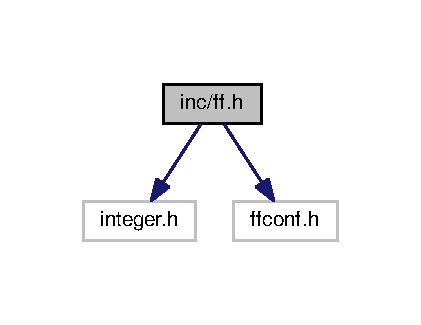
\includegraphics[width=202pt]{ff_8h__incl}
\end{center}
\end{figure}
This graph shows which files directly or indirectly include this file\+:
\nopagebreak
\begin{figure}[H]
\begin{center}
\leavevmode
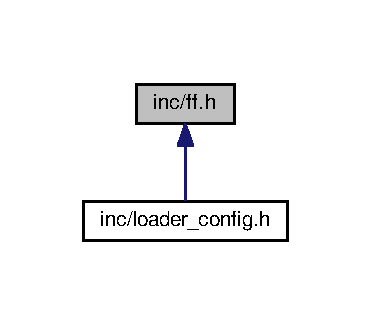
\includegraphics[width=178pt]{ff_8h__dep__incl}
\end{center}
\end{figure}
\subsection*{Data Structures}
\begin{DoxyCompactItemize}
\item 
struct \hyperlink{structFATFS}{F\+A\+T\+FS}
\begin{DoxyCompactList}\small\item\em File system object structure (\hyperlink{structFATFS}{F\+A\+T\+FS}) \end{DoxyCompactList}\item 
struct \hyperlink{structFIL}{F\+IL}
\begin{DoxyCompactList}\small\item\em File object structure (\hyperlink{structFIL}{F\+IL}) \end{DoxyCompactList}\item 
struct \hyperlink{structDIR}{D\+IR}
\begin{DoxyCompactList}\small\item\em Directory object structure (\hyperlink{structDIR}{D\+IR}) \end{DoxyCompactList}\item 
struct \hyperlink{structFILINFO}{F\+I\+L\+I\+N\+FO}
\begin{DoxyCompactList}\small\item\em File status structure (\hyperlink{structFILINFO}{F\+I\+L\+I\+N\+FO}) \end{DoxyCompactList}\end{DoxyCompactItemize}
\subsection*{Macros}
\begin{DoxyCompactItemize}
\item 
\#define {\bfseries \+\_\+\+F\+A\+T\+FS}~80376  /$\ast$ Revision ID $\ast$/\hypertarget{ff_8h_a749228947bc890224b8bd5de6e11faa3}{}\label{ff_8h_a749228947bc890224b8bd5de6e11faa3}

\item 
\#define {\bfseries L\+D2\+PD}(vol)~(B\+Y\+TE)(vol)  /$\ast$ Each logical drive is bound to the same physical drive number $\ast$/\hypertarget{ff_8h_a6577ed2f95527745bf4d27c53488b9a7}{}\label{ff_8h_a6577ed2f95527745bf4d27c53488b9a7}

\item 
\#define {\bfseries L\+D2\+PT}(vol)~0      /$\ast$ Find first valid partition or in S\+FD $\ast$/\hypertarget{ff_8h_aadc4a9aefaf2588bdd7565549f5d91e7}{}\label{ff_8h_aadc4a9aefaf2588bdd7565549f5d91e7}

\item 
\#define {\bfseries \+\_\+T}(x)~x\hypertarget{ff_8h_ae936e4c15227768f7da4e0951def89c8}{}\label{ff_8h_ae936e4c15227768f7da4e0951def89c8}

\item 
\#define {\bfseries \+\_\+\+T\+E\+XT}(x)~x\hypertarget{ff_8h_a3232964568d17bb4a1af30f9db826ce2}{}\label{ff_8h_a3232964568d17bb4a1af30f9db826ce2}

\item 
\#define {\bfseries f\+\_\+eof}(fp)~((int)((fp)-\/$>$fptr == (fp)-\/$>$fsize))\hypertarget{ff_8h_a970cdd8970a3a94967ad64cfc5d4c161}{}\label{ff_8h_a970cdd8970a3a94967ad64cfc5d4c161}

\item 
\#define {\bfseries f\+\_\+error}(fp)~((fp)-\/$>$err)\hypertarget{ff_8h_a25cbdabeed318802cf0e9db6671a33b7}{}\label{ff_8h_a25cbdabeed318802cf0e9db6671a33b7}

\item 
\#define {\bfseries f\+\_\+tell}(fp)~((fp)-\/$>$fptr)\hypertarget{ff_8h_a5e1daca7ce13cdc277e42185f7f9124f}{}\label{ff_8h_a5e1daca7ce13cdc277e42185f7f9124f}

\item 
\#define {\bfseries f\+\_\+size}(fp)~((fp)-\/$>$fsize)\hypertarget{ff_8h_a26f33722c5bf1aa3cd6f0290a83eb2bc}{}\label{ff_8h_a26f33722c5bf1aa3cd6f0290a83eb2bc}

\item 
\#define {\bfseries E\+OF}~(-\/1)\hypertarget{ff_8h_a59adc4c82490d23754cd39c2fb99b0da}{}\label{ff_8h_a59adc4c82490d23754cd39c2fb99b0da}

\item 
\#define {\bfseries F\+A\+\_\+\+R\+E\+AD}~0x01\hypertarget{ff_8h_a1f4f3530ff03abbd979b072536e72290}{}\label{ff_8h_a1f4f3530ff03abbd979b072536e72290}

\item 
\#define {\bfseries F\+A\+\_\+\+O\+P\+E\+N\+\_\+\+E\+X\+I\+S\+T\+I\+NG}~0x00\hypertarget{ff_8h_a0c5dd686b10f84c2a2b3954957a5979a}{}\label{ff_8h_a0c5dd686b10f84c2a2b3954957a5979a}

\item 
\#define {\bfseries F\+A\+\_\+\+W\+R\+I\+TE}~0x02\hypertarget{ff_8h_afa366963220c89b882c0361794020c14}{}\label{ff_8h_afa366963220c89b882c0361794020c14}

\item 
\#define {\bfseries F\+A\+\_\+\+C\+R\+E\+A\+T\+E\+\_\+\+N\+EW}~0x04\hypertarget{ff_8h_a417bb1babd1785fd181a806b5613eba3}{}\label{ff_8h_a417bb1babd1785fd181a806b5613eba3}

\item 
\#define {\bfseries F\+A\+\_\+\+C\+R\+E\+A\+T\+E\+\_\+\+A\+L\+W\+A\+YS}~0x08\hypertarget{ff_8h_afba4546b131dea4b24727fa20a80e29f}{}\label{ff_8h_afba4546b131dea4b24727fa20a80e29f}

\item 
\#define {\bfseries F\+A\+\_\+\+O\+P\+E\+N\+\_\+\+A\+L\+W\+A\+YS}~0x10\hypertarget{ff_8h_a17b01553029920ac0468912b4bcb16c7}{}\label{ff_8h_a17b01553029920ac0468912b4bcb16c7}

\item 
\#define {\bfseries F\+A\+\_\+\+\_\+\+W\+R\+I\+T\+T\+EN}~0x20\hypertarget{ff_8h_ac4b7d5223f84df91c306ffbff536fae4}{}\label{ff_8h_ac4b7d5223f84df91c306ffbff536fae4}

\item 
\#define {\bfseries F\+A\+\_\+\+\_\+\+D\+I\+R\+TY}~0x40\hypertarget{ff_8h_a5b2962e3616a1e9eb709d95f4c75c67c}{}\label{ff_8h_a5b2962e3616a1e9eb709d95f4c75c67c}

\item 
\#define {\bfseries F\+S\+\_\+\+F\+A\+T12}~1\hypertarget{ff_8h_aab755aa1b4f81f4aabee4a5d4738cfb0}{}\label{ff_8h_aab755aa1b4f81f4aabee4a5d4738cfb0}

\item 
\#define {\bfseries F\+S\+\_\+\+F\+A\+T16}~2\hypertarget{ff_8h_a7ef90a36d99edfc0138a2155a17a79b9}{}\label{ff_8h_a7ef90a36d99edfc0138a2155a17a79b9}

\item 
\#define {\bfseries F\+S\+\_\+\+F\+A\+T32}~3\hypertarget{ff_8h_ac63e0796095a789cefdbc3c3c676c9ce}{}\label{ff_8h_ac63e0796095a789cefdbc3c3c676c9ce}

\item 
\#define {\bfseries A\+M\+\_\+\+R\+DO}~0x01  /$\ast$ Read only $\ast$/\hypertarget{ff_8h_add6d85d1e7a02b4f6188783ef91a5f1e}{}\label{ff_8h_add6d85d1e7a02b4f6188783ef91a5f1e}

\item 
\#define {\bfseries A\+M\+\_\+\+H\+ID}~0x02  /$\ast$ Hidden $\ast$/\hypertarget{ff_8h_aa90c4c921c1955fd407d8bbf17f1674e}{}\label{ff_8h_aa90c4c921c1955fd407d8bbf17f1674e}

\item 
\#define {\bfseries A\+M\+\_\+\+S\+YS}~0x04  /$\ast$ System $\ast$/\hypertarget{ff_8h_a1f25d5c17b5a3a6397b3398add8cdc15}{}\label{ff_8h_a1f25d5c17b5a3a6397b3398add8cdc15}

\item 
\#define {\bfseries A\+M\+\_\+\+V\+OL}~0x08  /$\ast$ Volume label $\ast$/\hypertarget{ff_8h_a5cfae62dabae0a54809e43b36685ce7c}{}\label{ff_8h_a5cfae62dabae0a54809e43b36685ce7c}

\item 
\#define {\bfseries A\+M\+\_\+\+L\+FN}~0x0\+F  /$\ast$ L\+F\+N entry $\ast$/\hypertarget{ff_8h_a91161ef62e0e85ba3c2876d3d339473d}{}\label{ff_8h_a91161ef62e0e85ba3c2876d3d339473d}

\item 
\#define {\bfseries A\+M\+\_\+\+D\+IR}~0x10  /$\ast$ Directory $\ast$/\hypertarget{ff_8h_a3a9db44e978ed6c13b641e092d4cd7d3}{}\label{ff_8h_a3a9db44e978ed6c13b641e092d4cd7d3}

\item 
\#define {\bfseries A\+M\+\_\+\+A\+RC}~0x20  /$\ast$ Archive $\ast$/\hypertarget{ff_8h_ae8174d00798e34e7c9e95898cb9e1a09}{}\label{ff_8h_ae8174d00798e34e7c9e95898cb9e1a09}

\item 
\#define {\bfseries A\+M\+\_\+\+M\+A\+SK}~0x3\+F  /$\ast$ Mask of defined bits $\ast$/\hypertarget{ff_8h_aefa78fd6b130faaca4e115602869b57c}{}\label{ff_8h_aefa78fd6b130faaca4e115602869b57c}

\item 
\#define {\bfseries C\+R\+E\+A\+T\+E\+\_\+\+L\+I\+N\+K\+M\+AP}~0x\+F\+F\+F\+F\+F\+F\+FF\hypertarget{ff_8h_aee297a9011164cf485a4df2a72758b08}{}\label{ff_8h_aee297a9011164cf485a4df2a72758b08}

\item 
\#define {\bfseries L\+D\+\_\+\+W\+O\+RD}(ptr)~(W\+O\+RD)(((W\+O\+RD)$\ast$((B\+Y\+TE$\ast$)(ptr)+1)$<$$<$8)$\vert$(W\+O\+RD)$\ast$(B\+Y\+TE$\ast$)(ptr))\hypertarget{ff_8h_a398519bb08da6457e62567d1f0b567e3}{}\label{ff_8h_a398519bb08da6457e62567d1f0b567e3}

\item 
\#define {\bfseries L\+D\+\_\+\+D\+W\+O\+RD}(ptr)~(D\+W\+O\+RD)(((D\+W\+O\+RD)$\ast$((B\+Y\+TE$\ast$)(ptr)+3)$<$$<$24)$\vert$((D\+W\+O\+RD)$\ast$((B\+Y\+TE$\ast$)(ptr)+2)$<$$<$16)$\vert$((W\+O\+RD)$\ast$((B\+Y\+TE$\ast$)(ptr)+1)$<$$<$8)$\vert$$\ast$(B\+Y\+TE$\ast$)(ptr))\hypertarget{ff_8h_a4690304ddc975516f7dc02575c96e34e}{}\label{ff_8h_a4690304ddc975516f7dc02575c96e34e}

\item 
\#define {\bfseries S\+T\+\_\+\+W\+O\+RD}(ptr,  val)~$\ast$(B\+Y\+TE$\ast$)(ptr)=(B\+Y\+TE)(val); $\ast$((B\+Y\+TE$\ast$)(ptr)+1)=(B\+Y\+TE)((W\+O\+RD)(val)$>$$>$8)\hypertarget{ff_8h_a95ceb4c25b216e71baa7102939edfd0d}{}\label{ff_8h_a95ceb4c25b216e71baa7102939edfd0d}

\item 
\#define {\bfseries S\+T\+\_\+\+D\+W\+O\+RD}(ptr,  val)~$\ast$(B\+Y\+TE$\ast$)(ptr)=(B\+Y\+TE)(val); $\ast$((B\+Y\+TE$\ast$)(ptr)+1)=(B\+Y\+TE)((W\+O\+RD)(val)$>$$>$8); $\ast$((B\+Y\+TE$\ast$)(ptr)+2)=(B\+Y\+TE)((D\+W\+O\+RD)(val)$>$$>$16); $\ast$((B\+Y\+TE$\ast$)(ptr)+3)=(B\+Y\+TE)((D\+W\+O\+RD)(val)$>$$>$24)\hypertarget{ff_8h_abf5aba973d95ac5843b80aa7379cdd66}{}\label{ff_8h_abf5aba973d95ac5843b80aa7379cdd66}

\end{DoxyCompactItemize}
\subsection*{Typedefs}
\begin{DoxyCompactItemize}
\item 
typedef char {\bfseries T\+C\+H\+AR}\hypertarget{ff_8h_a03bdb8ce5895c7e261aadc2529637546}{}\label{ff_8h_a03bdb8ce5895c7e261aadc2529637546}

\end{DoxyCompactItemize}
\subsection*{Enumerations}
\begin{DoxyCompactItemize}
\item 
enum \hyperlink{ff_8h_a49d0171ecbd362cda5680a0d360db44c}{F\+R\+E\+S\+U\+LT} \{ \\*
{\bfseries F\+R\+\_\+\+OK} = 0, 
{\bfseries F\+R\+\_\+\+D\+I\+S\+K\+\_\+\+E\+RR}, 
{\bfseries F\+R\+\_\+\+I\+N\+T\+\_\+\+E\+RR}, 
{\bfseries F\+R\+\_\+\+N\+O\+T\+\_\+\+R\+E\+A\+DY}, 
\\*
{\bfseries F\+R\+\_\+\+N\+O\+\_\+\+F\+I\+LE}, 
{\bfseries F\+R\+\_\+\+N\+O\+\_\+\+P\+A\+TH}, 
{\bfseries F\+R\+\_\+\+I\+N\+V\+A\+L\+I\+D\+\_\+\+N\+A\+ME}, 
{\bfseries F\+R\+\_\+\+D\+E\+N\+I\+ED}, 
\\*
{\bfseries F\+R\+\_\+\+E\+X\+I\+ST}, 
{\bfseries F\+R\+\_\+\+I\+N\+V\+A\+L\+I\+D\+\_\+\+O\+B\+J\+E\+CT}, 
{\bfseries F\+R\+\_\+\+W\+R\+I\+T\+E\+\_\+\+P\+R\+O\+T\+E\+C\+T\+ED}, 
{\bfseries F\+R\+\_\+\+I\+N\+V\+A\+L\+I\+D\+\_\+\+D\+R\+I\+VE}, 
\\*
{\bfseries F\+R\+\_\+\+N\+O\+T\+\_\+\+E\+N\+A\+B\+L\+ED}, 
{\bfseries F\+R\+\_\+\+N\+O\+\_\+\+F\+I\+L\+E\+S\+Y\+S\+T\+EM}, 
{\bfseries F\+R\+\_\+\+M\+K\+F\+S\+\_\+\+A\+B\+O\+R\+T\+ED}, 
{\bfseries F\+R\+\_\+\+T\+I\+M\+E\+O\+UT}, 
\\*
{\bfseries F\+R\+\_\+\+L\+O\+C\+K\+ED}, 
{\bfseries F\+R\+\_\+\+N\+O\+T\+\_\+\+E\+N\+O\+U\+G\+H\+\_\+\+C\+O\+RE}, 
{\bfseries F\+R\+\_\+\+T\+O\+O\+\_\+\+M\+A\+N\+Y\+\_\+\+O\+P\+E\+N\+\_\+\+F\+I\+L\+ES}, 
{\bfseries F\+R\+\_\+\+I\+N\+V\+A\+L\+I\+D\+\_\+\+P\+A\+R\+A\+M\+E\+T\+ER}
 \}\hypertarget{ff_8h_a49d0171ecbd362cda5680a0d360db44c}{}\label{ff_8h_a49d0171ecbd362cda5680a0d360db44c}
\begin{DoxyCompactList}\small\item\em File function return code (F\+R\+E\+S\+U\+LT) \end{DoxyCompactList}
\end{DoxyCompactItemize}
\subsection*{Functions}
\begin{DoxyCompactItemize}
\item 
\hyperlink{ff_8h_a49d0171ecbd362cda5680a0d360db44c}{F\+R\+E\+S\+U\+LT} \hyperlink{ff_8h_aefdef7126128d99d0b3bd82c28e54d80}{f\+\_\+open} (\hyperlink{structFIL}{F\+IL} $\ast$fp, const T\+C\+H\+AR $\ast$path, B\+Y\+TE mode)
\item 
\hyperlink{ff_8h_a49d0171ecbd362cda5680a0d360db44c}{F\+R\+E\+S\+U\+LT} \hyperlink{ff_8h_a53882db20ef4323dcfd1874d7733ffc3}{f\+\_\+close} (\hyperlink{structFIL}{F\+IL} $\ast$fp)
\item 
\hyperlink{ff_8h_a49d0171ecbd362cda5680a0d360db44c}{F\+R\+E\+S\+U\+LT} \hyperlink{ff_8h_ac4c3dcb6869ca252888eebabe39727b3}{f\+\_\+read} (\hyperlink{structFIL}{F\+IL} $\ast$fp, void $\ast$buff, U\+I\+NT btr, U\+I\+NT $\ast$br)
\item 
\hyperlink{ff_8h_a49d0171ecbd362cda5680a0d360db44c}{F\+R\+E\+S\+U\+LT} \hyperlink{ff_8h_ae6a4dfae8a9e308bdb2283a37ef680f2}{f\+\_\+write} (\hyperlink{structFIL}{F\+IL} $\ast$fp, const void $\ast$buff, U\+I\+NT btw, U\+I\+NT $\ast$bw)
\item 
\hyperlink{ff_8h_a49d0171ecbd362cda5680a0d360db44c}{F\+R\+E\+S\+U\+LT} \hyperlink{ff_8h_a6c0c4cd695704aa6d952c90be81d9849}{f\+\_\+forward} (\hyperlink{structFIL}{F\+IL} $\ast$fp, U\+I\+NT($\ast$func)(const B\+Y\+TE $\ast$, U\+I\+NT), U\+I\+NT btf, U\+I\+NT $\ast$bf)
\item 
\hyperlink{ff_8h_a49d0171ecbd362cda5680a0d360db44c}{F\+R\+E\+S\+U\+LT} \hyperlink{ff_8h_a5df0ac672ada972e89ef4b003e57f964}{f\+\_\+lseek} (\hyperlink{structFIL}{F\+IL} $\ast$fp, D\+W\+O\+RD ofs)
\item 
\hyperlink{ff_8h_a49d0171ecbd362cda5680a0d360db44c}{F\+R\+E\+S\+U\+LT} \hyperlink{ff_8h_a691a27b40c348f7c84b42e911636f38a}{f\+\_\+truncate} (\hyperlink{structFIL}{F\+IL} $\ast$fp)
\item 
\hyperlink{ff_8h_a49d0171ecbd362cda5680a0d360db44c}{F\+R\+E\+S\+U\+LT} \hyperlink{ff_8h_ad69c7246b122ba56a134939ee0eaf847}{f\+\_\+sync} (\hyperlink{structFIL}{F\+IL} $\ast$fp)
\item 
\hyperlink{ff_8h_a49d0171ecbd362cda5680a0d360db44c}{F\+R\+E\+S\+U\+LT} \hyperlink{ff_8h_ab63b213c75f7335fbb63a1f3f70e5fc7}{f\+\_\+opendir} (\hyperlink{structDIR}{D\+IR} $\ast$dp, const T\+C\+H\+AR $\ast$path)
\item 
\hyperlink{ff_8h_a49d0171ecbd362cda5680a0d360db44c}{F\+R\+E\+S\+U\+LT} \hyperlink{ff_8h_ab5f7376b6f3e3bcc7f5ff5497c8b7364}{f\+\_\+closedir} (\hyperlink{structDIR}{D\+IR} $\ast$dp)
\item 
\hyperlink{ff_8h_a49d0171ecbd362cda5680a0d360db44c}{F\+R\+E\+S\+U\+LT} \hyperlink{ff_8h_ab39e82a110695de45f416f3149358012}{f\+\_\+readdir} (\hyperlink{structDIR}{D\+IR} $\ast$dp, \hyperlink{structFILINFO}{F\+I\+L\+I\+N\+FO} $\ast$fno)
\item 
\hyperlink{ff_8h_a49d0171ecbd362cda5680a0d360db44c}{F\+R\+E\+S\+U\+LT} \hyperlink{ff_8h_a4b4d38db58e89c526cfcf53200d719d0}{f\+\_\+mkdir} (const T\+C\+H\+AR $\ast$path)
\item 
\hyperlink{ff_8h_a49d0171ecbd362cda5680a0d360db44c}{F\+R\+E\+S\+U\+LT} \hyperlink{ff_8h_a2858167fcd0bced48e9be434b3895efe}{f\+\_\+unlink} (const T\+C\+H\+AR $\ast$path)
\item 
\hyperlink{ff_8h_a49d0171ecbd362cda5680a0d360db44c}{F\+R\+E\+S\+U\+LT} \hyperlink{ff_8h_aa775b9b024acfeb3a66523cab497d142}{f\+\_\+rename} (const T\+C\+H\+AR $\ast$path\+\_\+old, const T\+C\+H\+AR $\ast$path\+\_\+new)
\item 
\hyperlink{ff_8h_a49d0171ecbd362cda5680a0d360db44c}{F\+R\+E\+S\+U\+LT} \hyperlink{ff_8h_abe1f60daab5c7d11170c334fb832c798}{f\+\_\+stat} (const T\+C\+H\+AR $\ast$path, \hyperlink{structFILINFO}{F\+I\+L\+I\+N\+FO} $\ast$fno)
\item 
\hyperlink{ff_8h_a49d0171ecbd362cda5680a0d360db44c}{F\+R\+E\+S\+U\+LT} \hyperlink{ff_8h_ab60b118acf7efa6ea19abb5db05ecccb}{f\+\_\+chmod} (const T\+C\+H\+AR $\ast$path, B\+Y\+TE value, B\+Y\+TE mask)
\item 
\hyperlink{ff_8h_a49d0171ecbd362cda5680a0d360db44c}{F\+R\+E\+S\+U\+LT} \hyperlink{ff_8h_aafaa718d1a487e12a8f0087173dba0b9}{f\+\_\+utime} (const T\+C\+H\+AR $\ast$path, const \hyperlink{structFILINFO}{F\+I\+L\+I\+N\+FO} $\ast$fno)
\item 
\hyperlink{ff_8h_a49d0171ecbd362cda5680a0d360db44c}{F\+R\+E\+S\+U\+LT} \hyperlink{ff_8h_a53c7e9a7fb3c279254cd2d0445667e2f}{f\+\_\+chdir} (const T\+C\+H\+AR $\ast$path)
\item 
\hyperlink{ff_8h_a49d0171ecbd362cda5680a0d360db44c}{F\+R\+E\+S\+U\+LT} \hyperlink{ff_8h_a13e5933f851b436890361189f64261cd}{f\+\_\+chdrive} (const T\+C\+H\+AR $\ast$path)
\item 
\hyperlink{ff_8h_a49d0171ecbd362cda5680a0d360db44c}{F\+R\+E\+S\+U\+LT} \hyperlink{ff_8h_acb865a03dbac0031ac5cb8a031f7b71c}{f\+\_\+getcwd} (T\+C\+H\+AR $\ast$buff, U\+I\+NT len)
\item 
\hyperlink{ff_8h_a49d0171ecbd362cda5680a0d360db44c}{F\+R\+E\+S\+U\+LT} \hyperlink{ff_8h_a0ff39f75a87cbda9cd6ea65d83f16cec}{f\+\_\+getfree} (const T\+C\+H\+AR $\ast$path, D\+W\+O\+RD $\ast$nclst, \hyperlink{structFATFS}{F\+A\+T\+FS} $\ast$$\ast$fatfs)
\item 
\hyperlink{ff_8h_a49d0171ecbd362cda5680a0d360db44c}{F\+R\+E\+S\+U\+LT} \hyperlink{ff_8h_ac4ff40a674bcbfe40d81b1e8e54befc6}{f\+\_\+getlabel} (const T\+C\+H\+AR $\ast$path, T\+C\+H\+AR $\ast$label, D\+W\+O\+RD $\ast$vsn)
\item 
\hyperlink{ff_8h_a49d0171ecbd362cda5680a0d360db44c}{F\+R\+E\+S\+U\+LT} \hyperlink{ff_8h_aa82bca64e28bc0d656a7999dd0eadec7}{f\+\_\+setlabel} (const T\+C\+H\+AR $\ast$label)
\item 
\hyperlink{ff_8h_a49d0171ecbd362cda5680a0d360db44c}{F\+R\+E\+S\+U\+LT} \hyperlink{ff_8h_a16a934c2bbfa2160295810adc49d5509}{f\+\_\+mount} (\hyperlink{structFATFS}{F\+A\+T\+FS} $\ast$fs, const T\+C\+H\+AR $\ast$path, B\+Y\+TE opt)
\item 
\hyperlink{ff_8h_a49d0171ecbd362cda5680a0d360db44c}{F\+R\+E\+S\+U\+LT} \hyperlink{ff_8h_a799aff9594e708c8be357281cf85428b}{f\+\_\+mkfs} (const T\+C\+H\+AR $\ast$path, B\+Y\+TE sfd, U\+I\+NT au)
\item 
\hyperlink{ff_8h_a49d0171ecbd362cda5680a0d360db44c}{F\+R\+E\+S\+U\+LT} \hyperlink{ff_8h_ae89e589480ab573ce19d22dcd022efe0}{f\+\_\+fdisk} (B\+Y\+TE pdrv, const D\+W\+O\+RD szt\mbox{[}$\,$\mbox{]}, void $\ast$work)
\item 
int \hyperlink{ff_8h_ad1d73b8d01c2ef89eddf920b7fcc6beb}{f\+\_\+putc} (T\+C\+H\+AR c, \hyperlink{structFIL}{F\+IL} $\ast$fp)
\item 
int \hyperlink{ff_8h_a699fc03ffa785ceab8812a7f204421f3}{f\+\_\+puts} (const T\+C\+H\+AR $\ast$str, \hyperlink{structFIL}{F\+IL} $\ast$cp)
\item 
int \hyperlink{ff_8h_a4ce26253177c167df849e76f69b5c66c}{f\+\_\+printf} (\hyperlink{structFIL}{F\+IL} $\ast$fp, const T\+C\+H\+AR $\ast$str,...)
\item 
T\+C\+H\+AR $\ast$ \hyperlink{ff_8h_a0fa54bd310785ecdaed19dda8f60dac5}{f\+\_\+gets} (T\+C\+H\+AR $\ast$buff, int len, \hyperlink{structFIL}{F\+IL} $\ast$fp)
\end{DoxyCompactItemize}


\subsection{Detailed Description}
Fat\+Fs -\/ F\+AT file system module include file R0.\+10c (C)ChaN, 2014 Fat\+Fs module is a generic F\+AT file system module for small embedded systems. This is a free software that opened for education, research and commercial developments under license policy of following terms. Copyright (C) 2014, , all right reserved. The Fat\+Fs module is a free software and there is NO W\+A\+R\+R\+A\+N\+TY. No restriction on use. You can use, modify and redistribute it for personal, non-\/profit or commercial product U\+N\+D\+ER Y\+O\+UR R\+E\+S\+P\+O\+N\+S\+I\+B\+I\+L\+I\+TY. Redistributions of source code must retain the above copyright notice. 

\begin{DoxyAuthor}{Author}
ChaN 
\end{DoxyAuthor}


\subsection{Function Documentation}
\index{ff.\+h@{ff.\+h}!f\+\_\+chdir@{f\+\_\+chdir}}
\index{f\+\_\+chdir@{f\+\_\+chdir}!ff.\+h@{ff.\+h}}
\subsubsection[{\texorpdfstring{f\+\_\+chdir(const T\+C\+H\+A\+R $\ast$path)}{f_chdir(const TCHAR *path)}}]{\setlength{\rightskip}{0pt plus 5cm}{\bf F\+R\+E\+S\+U\+LT} f\+\_\+chdir (
\begin{DoxyParamCaption}
\item[{const T\+C\+H\+AR $\ast$}]{path}
\end{DoxyParamCaption}
)}\hypertarget{ff_8h_a53c7e9a7fb3c279254cd2d0445667e2f}{}\label{ff_8h_a53c7e9a7fb3c279254cd2d0445667e2f}
Change current directory \index{ff.\+h@{ff.\+h}!f\+\_\+chdrive@{f\+\_\+chdrive}}
\index{f\+\_\+chdrive@{f\+\_\+chdrive}!ff.\+h@{ff.\+h}}
\subsubsection[{\texorpdfstring{f\+\_\+chdrive(const T\+C\+H\+A\+R $\ast$path)}{f_chdrive(const TCHAR *path)}}]{\setlength{\rightskip}{0pt plus 5cm}{\bf F\+R\+E\+S\+U\+LT} f\+\_\+chdrive (
\begin{DoxyParamCaption}
\item[{const T\+C\+H\+AR $\ast$}]{path}
\end{DoxyParamCaption}
)}\hypertarget{ff_8h_a13e5933f851b436890361189f64261cd}{}\label{ff_8h_a13e5933f851b436890361189f64261cd}
Change current drive \index{ff.\+h@{ff.\+h}!f\+\_\+chmod@{f\+\_\+chmod}}
\index{f\+\_\+chmod@{f\+\_\+chmod}!ff.\+h@{ff.\+h}}
\subsubsection[{\texorpdfstring{f\+\_\+chmod(const T\+C\+H\+A\+R $\ast$path, B\+Y\+T\+E value, B\+Y\+T\+E mask)}{f_chmod(const TCHAR *path, BYTE value, BYTE mask)}}]{\setlength{\rightskip}{0pt plus 5cm}{\bf F\+R\+E\+S\+U\+LT} f\+\_\+chmod (
\begin{DoxyParamCaption}
\item[{const T\+C\+H\+AR $\ast$}]{path, }
\item[{B\+Y\+TE}]{value, }
\item[{B\+Y\+TE}]{mask}
\end{DoxyParamCaption}
)}\hypertarget{ff_8h_ab60b118acf7efa6ea19abb5db05ecccb}{}\label{ff_8h_ab60b118acf7efa6ea19abb5db05ecccb}
Change attribute of the file/dir \index{ff.\+h@{ff.\+h}!f\+\_\+close@{f\+\_\+close}}
\index{f\+\_\+close@{f\+\_\+close}!ff.\+h@{ff.\+h}}
\subsubsection[{\texorpdfstring{f\+\_\+close(\+F\+I\+L $\ast$fp)}{f_close(FIL *fp)}}]{\setlength{\rightskip}{0pt plus 5cm}{\bf F\+R\+E\+S\+U\+LT} f\+\_\+close (
\begin{DoxyParamCaption}
\item[{{\bf F\+IL} $\ast$}]{fp}
\end{DoxyParamCaption}
)}\hypertarget{ff_8h_a53882db20ef4323dcfd1874d7733ffc3}{}\label{ff_8h_a53882db20ef4323dcfd1874d7733ffc3}
Close an open file object \index{ff.\+h@{ff.\+h}!f\+\_\+closedir@{f\+\_\+closedir}}
\index{f\+\_\+closedir@{f\+\_\+closedir}!ff.\+h@{ff.\+h}}
\subsubsection[{\texorpdfstring{f\+\_\+closedir(\+D\+I\+R $\ast$dp)}{f_closedir(DIR *dp)}}]{\setlength{\rightskip}{0pt plus 5cm}{\bf F\+R\+E\+S\+U\+LT} f\+\_\+closedir (
\begin{DoxyParamCaption}
\item[{{\bf D\+IR} $\ast$}]{dp}
\end{DoxyParamCaption}
)}\hypertarget{ff_8h_ab5f7376b6f3e3bcc7f5ff5497c8b7364}{}\label{ff_8h_ab5f7376b6f3e3bcc7f5ff5497c8b7364}
Close an open directory \index{ff.\+h@{ff.\+h}!f\+\_\+fdisk@{f\+\_\+fdisk}}
\index{f\+\_\+fdisk@{f\+\_\+fdisk}!ff.\+h@{ff.\+h}}
\subsubsection[{\texorpdfstring{f\+\_\+fdisk(\+B\+Y\+T\+E pdrv, const D\+W\+O\+R\+D szt[], void $\ast$work)}{f_fdisk(BYTE pdrv, const DWORD szt[], void *work)}}]{\setlength{\rightskip}{0pt plus 5cm}{\bf F\+R\+E\+S\+U\+LT} f\+\_\+fdisk (
\begin{DoxyParamCaption}
\item[{B\+Y\+TE}]{pdrv, }
\item[{const D\+W\+O\+RD}]{szt\mbox{[}$\,$\mbox{]}, }
\item[{void $\ast$}]{work}
\end{DoxyParamCaption}
)}\hypertarget{ff_8h_ae89e589480ab573ce19d22dcd022efe0}{}\label{ff_8h_ae89e589480ab573ce19d22dcd022efe0}
Divide a physical drive into some partitions \index{ff.\+h@{ff.\+h}!f\+\_\+forward@{f\+\_\+forward}}
\index{f\+\_\+forward@{f\+\_\+forward}!ff.\+h@{ff.\+h}}
\subsubsection[{\texorpdfstring{f\+\_\+forward(\+F\+I\+L $\ast$fp, U\+I\+N\+T($\ast$func)(const B\+Y\+T\+E $\ast$, U\+I\+N\+T), U\+I\+N\+T btf, U\+I\+N\+T $\ast$bf)}{f_forward(FIL *fp, UINT(*func)(const BYTE *, UINT), UINT btf, UINT *bf)}}]{\setlength{\rightskip}{0pt plus 5cm}{\bf F\+R\+E\+S\+U\+LT} f\+\_\+forward (
\begin{DoxyParamCaption}
\item[{{\bf F\+IL} $\ast$}]{fp, }
\item[{U\+I\+NT($\ast$)(const B\+Y\+TE $\ast$, U\+I\+NT)}]{func, }
\item[{U\+I\+NT}]{btf, }
\item[{U\+I\+NT $\ast$}]{bf}
\end{DoxyParamCaption}
)}\hypertarget{ff_8h_a6c0c4cd695704aa6d952c90be81d9849}{}\label{ff_8h_a6c0c4cd695704aa6d952c90be81d9849}
Forward data to the stream \index{ff.\+h@{ff.\+h}!f\+\_\+getcwd@{f\+\_\+getcwd}}
\index{f\+\_\+getcwd@{f\+\_\+getcwd}!ff.\+h@{ff.\+h}}
\subsubsection[{\texorpdfstring{f\+\_\+getcwd(\+T\+C\+H\+A\+R $\ast$buff, U\+I\+N\+T len)}{f_getcwd(TCHAR *buff, UINT len)}}]{\setlength{\rightskip}{0pt plus 5cm}{\bf F\+R\+E\+S\+U\+LT} f\+\_\+getcwd (
\begin{DoxyParamCaption}
\item[{T\+C\+H\+AR $\ast$}]{buff, }
\item[{U\+I\+NT}]{len}
\end{DoxyParamCaption}
)}\hypertarget{ff_8h_acb865a03dbac0031ac5cb8a031f7b71c}{}\label{ff_8h_acb865a03dbac0031ac5cb8a031f7b71c}
Get current directory \index{ff.\+h@{ff.\+h}!f\+\_\+getfree@{f\+\_\+getfree}}
\index{f\+\_\+getfree@{f\+\_\+getfree}!ff.\+h@{ff.\+h}}
\subsubsection[{\texorpdfstring{f\+\_\+getfree(const T\+C\+H\+A\+R $\ast$path, D\+W\+O\+R\+D $\ast$nclst, F\+A\+T\+F\+S $\ast$$\ast$fatfs)}{f_getfree(const TCHAR *path, DWORD *nclst, FATFS **fatfs)}}]{\setlength{\rightskip}{0pt plus 5cm}{\bf F\+R\+E\+S\+U\+LT} f\+\_\+getfree (
\begin{DoxyParamCaption}
\item[{const T\+C\+H\+AR $\ast$}]{path, }
\item[{D\+W\+O\+RD $\ast$}]{nclst, }
\item[{{\bf F\+A\+T\+FS} $\ast$$\ast$}]{fatfs}
\end{DoxyParamCaption}
)}\hypertarget{ff_8h_a0ff39f75a87cbda9cd6ea65d83f16cec}{}\label{ff_8h_a0ff39f75a87cbda9cd6ea65d83f16cec}
Get number of free clusters on the drive \index{ff.\+h@{ff.\+h}!f\+\_\+getlabel@{f\+\_\+getlabel}}
\index{f\+\_\+getlabel@{f\+\_\+getlabel}!ff.\+h@{ff.\+h}}
\subsubsection[{\texorpdfstring{f\+\_\+getlabel(const T\+C\+H\+A\+R $\ast$path, T\+C\+H\+A\+R $\ast$label, D\+W\+O\+R\+D $\ast$vsn)}{f_getlabel(const TCHAR *path, TCHAR *label, DWORD *vsn)}}]{\setlength{\rightskip}{0pt plus 5cm}{\bf F\+R\+E\+S\+U\+LT} f\+\_\+getlabel (
\begin{DoxyParamCaption}
\item[{const T\+C\+H\+AR $\ast$}]{path, }
\item[{T\+C\+H\+AR $\ast$}]{label, }
\item[{D\+W\+O\+RD $\ast$}]{vsn}
\end{DoxyParamCaption}
)}\hypertarget{ff_8h_ac4ff40a674bcbfe40d81b1e8e54befc6}{}\label{ff_8h_ac4ff40a674bcbfe40d81b1e8e54befc6}
Get volume label \index{ff.\+h@{ff.\+h}!f\+\_\+gets@{f\+\_\+gets}}
\index{f\+\_\+gets@{f\+\_\+gets}!ff.\+h@{ff.\+h}}
\subsubsection[{\texorpdfstring{f\+\_\+gets(\+T\+C\+H\+A\+R $\ast$buff, int len, F\+I\+L $\ast$fp)}{f_gets(TCHAR *buff, int len, FIL *fp)}}]{\setlength{\rightskip}{0pt plus 5cm}T\+C\+H\+AR$\ast$ f\+\_\+gets (
\begin{DoxyParamCaption}
\item[{T\+C\+H\+AR $\ast$}]{buff, }
\item[{int}]{len, }
\item[{{\bf F\+IL} $\ast$}]{fp}
\end{DoxyParamCaption}
)}\hypertarget{ff_8h_a0fa54bd310785ecdaed19dda8f60dac5}{}\label{ff_8h_a0fa54bd310785ecdaed19dda8f60dac5}
Get a string from the file \index{ff.\+h@{ff.\+h}!f\+\_\+lseek@{f\+\_\+lseek}}
\index{f\+\_\+lseek@{f\+\_\+lseek}!ff.\+h@{ff.\+h}}
\subsubsection[{\texorpdfstring{f\+\_\+lseek(\+F\+I\+L $\ast$fp, D\+W\+O\+R\+D ofs)}{f_lseek(FIL *fp, DWORD ofs)}}]{\setlength{\rightskip}{0pt plus 5cm}{\bf F\+R\+E\+S\+U\+LT} f\+\_\+lseek (
\begin{DoxyParamCaption}
\item[{{\bf F\+IL} $\ast$}]{fp, }
\item[{D\+W\+O\+RD}]{ofs}
\end{DoxyParamCaption}
)}\hypertarget{ff_8h_a5df0ac672ada972e89ef4b003e57f964}{}\label{ff_8h_a5df0ac672ada972e89ef4b003e57f964}
Move file pointer of a file object \index{ff.\+h@{ff.\+h}!f\+\_\+mkdir@{f\+\_\+mkdir}}
\index{f\+\_\+mkdir@{f\+\_\+mkdir}!ff.\+h@{ff.\+h}}
\subsubsection[{\texorpdfstring{f\+\_\+mkdir(const T\+C\+H\+A\+R $\ast$path)}{f_mkdir(const TCHAR *path)}}]{\setlength{\rightskip}{0pt plus 5cm}{\bf F\+R\+E\+S\+U\+LT} f\+\_\+mkdir (
\begin{DoxyParamCaption}
\item[{const T\+C\+H\+AR $\ast$}]{path}
\end{DoxyParamCaption}
)}\hypertarget{ff_8h_a4b4d38db58e89c526cfcf53200d719d0}{}\label{ff_8h_a4b4d38db58e89c526cfcf53200d719d0}
Create a sub directory \index{ff.\+h@{ff.\+h}!f\+\_\+mkfs@{f\+\_\+mkfs}}
\index{f\+\_\+mkfs@{f\+\_\+mkfs}!ff.\+h@{ff.\+h}}
\subsubsection[{\texorpdfstring{f\+\_\+mkfs(const T\+C\+H\+A\+R $\ast$path, B\+Y\+T\+E sfd, U\+I\+N\+T au)}{f_mkfs(const TCHAR *path, BYTE sfd, UINT au)}}]{\setlength{\rightskip}{0pt plus 5cm}{\bf F\+R\+E\+S\+U\+LT} f\+\_\+mkfs (
\begin{DoxyParamCaption}
\item[{const T\+C\+H\+AR $\ast$}]{path, }
\item[{B\+Y\+TE}]{sfd, }
\item[{U\+I\+NT}]{au}
\end{DoxyParamCaption}
)}\hypertarget{ff_8h_a799aff9594e708c8be357281cf85428b}{}\label{ff_8h_a799aff9594e708c8be357281cf85428b}
Create a file system on the volume \index{ff.\+h@{ff.\+h}!f\+\_\+mount@{f\+\_\+mount}}
\index{f\+\_\+mount@{f\+\_\+mount}!ff.\+h@{ff.\+h}}
\subsubsection[{\texorpdfstring{f\+\_\+mount(\+F\+A\+T\+F\+S $\ast$fs, const T\+C\+H\+A\+R $\ast$path, B\+Y\+T\+E opt)}{f_mount(FATFS *fs, const TCHAR *path, BYTE opt)}}]{\setlength{\rightskip}{0pt plus 5cm}{\bf F\+R\+E\+S\+U\+LT} f\+\_\+mount (
\begin{DoxyParamCaption}
\item[{{\bf F\+A\+T\+FS} $\ast$}]{fs, }
\item[{const T\+C\+H\+AR $\ast$}]{path, }
\item[{B\+Y\+TE}]{opt}
\end{DoxyParamCaption}
)}\hypertarget{ff_8h_a16a934c2bbfa2160295810adc49d5509}{}\label{ff_8h_a16a934c2bbfa2160295810adc49d5509}
Mount/\+Unmount a logical drive \index{ff.\+h@{ff.\+h}!f\+\_\+open@{f\+\_\+open}}
\index{f\+\_\+open@{f\+\_\+open}!ff.\+h@{ff.\+h}}
\subsubsection[{\texorpdfstring{f\+\_\+open(\+F\+I\+L $\ast$fp, const T\+C\+H\+A\+R $\ast$path, B\+Y\+T\+E mode)}{f_open(FIL *fp, const TCHAR *path, BYTE mode)}}]{\setlength{\rightskip}{0pt plus 5cm}{\bf F\+R\+E\+S\+U\+LT} f\+\_\+open (
\begin{DoxyParamCaption}
\item[{{\bf F\+IL} $\ast$}]{fp, }
\item[{const T\+C\+H\+AR $\ast$}]{path, }
\item[{B\+Y\+TE}]{mode}
\end{DoxyParamCaption}
)}\hypertarget{ff_8h_aefdef7126128d99d0b3bd82c28e54d80}{}\label{ff_8h_aefdef7126128d99d0b3bd82c28e54d80}
Open or create a file \index{ff.\+h@{ff.\+h}!f\+\_\+opendir@{f\+\_\+opendir}}
\index{f\+\_\+opendir@{f\+\_\+opendir}!ff.\+h@{ff.\+h}}
\subsubsection[{\texorpdfstring{f\+\_\+opendir(\+D\+I\+R $\ast$dp, const T\+C\+H\+A\+R $\ast$path)}{f_opendir(DIR *dp, const TCHAR *path)}}]{\setlength{\rightskip}{0pt plus 5cm}{\bf F\+R\+E\+S\+U\+LT} f\+\_\+opendir (
\begin{DoxyParamCaption}
\item[{{\bf D\+IR} $\ast$}]{dp, }
\item[{const T\+C\+H\+AR $\ast$}]{path}
\end{DoxyParamCaption}
)}\hypertarget{ff_8h_ab63b213c75f7335fbb63a1f3f70e5fc7}{}\label{ff_8h_ab63b213c75f7335fbb63a1f3f70e5fc7}
Open a directory \index{ff.\+h@{ff.\+h}!f\+\_\+printf@{f\+\_\+printf}}
\index{f\+\_\+printf@{f\+\_\+printf}!ff.\+h@{ff.\+h}}
\subsubsection[{\texorpdfstring{f\+\_\+printf(\+F\+I\+L $\ast$fp, const T\+C\+H\+A\+R $\ast$str,...)}{f_printf(FIL *fp, const TCHAR *str,...)}}]{\setlength{\rightskip}{0pt plus 5cm}int f\+\_\+printf (
\begin{DoxyParamCaption}
\item[{{\bf F\+IL} $\ast$}]{fp, }
\item[{const T\+C\+H\+AR $\ast$}]{str, }
\item[{}]{...}
\end{DoxyParamCaption}
)}\hypertarget{ff_8h_a4ce26253177c167df849e76f69b5c66c}{}\label{ff_8h_a4ce26253177c167df849e76f69b5c66c}
Put a formatted string to the file \index{ff.\+h@{ff.\+h}!f\+\_\+putc@{f\+\_\+putc}}
\index{f\+\_\+putc@{f\+\_\+putc}!ff.\+h@{ff.\+h}}
\subsubsection[{\texorpdfstring{f\+\_\+putc(\+T\+C\+H\+A\+R c, F\+I\+L $\ast$fp)}{f_putc(TCHAR c, FIL *fp)}}]{\setlength{\rightskip}{0pt plus 5cm}int f\+\_\+putc (
\begin{DoxyParamCaption}
\item[{T\+C\+H\+AR}]{c, }
\item[{{\bf F\+IL} $\ast$}]{fp}
\end{DoxyParamCaption}
)}\hypertarget{ff_8h_ad1d73b8d01c2ef89eddf920b7fcc6beb}{}\label{ff_8h_ad1d73b8d01c2ef89eddf920b7fcc6beb}
Put a character to the file \index{ff.\+h@{ff.\+h}!f\+\_\+puts@{f\+\_\+puts}}
\index{f\+\_\+puts@{f\+\_\+puts}!ff.\+h@{ff.\+h}}
\subsubsection[{\texorpdfstring{f\+\_\+puts(const T\+C\+H\+A\+R $\ast$str, F\+I\+L $\ast$cp)}{f_puts(const TCHAR *str, FIL *cp)}}]{\setlength{\rightskip}{0pt plus 5cm}int f\+\_\+puts (
\begin{DoxyParamCaption}
\item[{const T\+C\+H\+AR $\ast$}]{str, }
\item[{{\bf F\+IL} $\ast$}]{cp}
\end{DoxyParamCaption}
)}\hypertarget{ff_8h_a699fc03ffa785ceab8812a7f204421f3}{}\label{ff_8h_a699fc03ffa785ceab8812a7f204421f3}
Put a string to the file \index{ff.\+h@{ff.\+h}!f\+\_\+read@{f\+\_\+read}}
\index{f\+\_\+read@{f\+\_\+read}!ff.\+h@{ff.\+h}}
\subsubsection[{\texorpdfstring{f\+\_\+read(\+F\+I\+L $\ast$fp, void $\ast$buff, U\+I\+N\+T btr, U\+I\+N\+T $\ast$br)}{f_read(FIL *fp, void *buff, UINT btr, UINT *br)}}]{\setlength{\rightskip}{0pt plus 5cm}{\bf F\+R\+E\+S\+U\+LT} f\+\_\+read (
\begin{DoxyParamCaption}
\item[{{\bf F\+IL} $\ast$}]{fp, }
\item[{void $\ast$}]{buff, }
\item[{U\+I\+NT}]{btr, }
\item[{U\+I\+NT $\ast$}]{br}
\end{DoxyParamCaption}
)}\hypertarget{ff_8h_ac4c3dcb6869ca252888eebabe39727b3}{}\label{ff_8h_ac4c3dcb6869ca252888eebabe39727b3}
Read data from a file \index{ff.\+h@{ff.\+h}!f\+\_\+readdir@{f\+\_\+readdir}}
\index{f\+\_\+readdir@{f\+\_\+readdir}!ff.\+h@{ff.\+h}}
\subsubsection[{\texorpdfstring{f\+\_\+readdir(\+D\+I\+R $\ast$dp, F\+I\+L\+I\+N\+F\+O $\ast$fno)}{f_readdir(DIR *dp, FILINFO *fno)}}]{\setlength{\rightskip}{0pt plus 5cm}{\bf F\+R\+E\+S\+U\+LT} f\+\_\+readdir (
\begin{DoxyParamCaption}
\item[{{\bf D\+IR} $\ast$}]{dp, }
\item[{{\bf F\+I\+L\+I\+N\+FO} $\ast$}]{fno}
\end{DoxyParamCaption}
)}\hypertarget{ff_8h_ab39e82a110695de45f416f3149358012}{}\label{ff_8h_ab39e82a110695de45f416f3149358012}
Read a directory item \index{ff.\+h@{ff.\+h}!f\+\_\+rename@{f\+\_\+rename}}
\index{f\+\_\+rename@{f\+\_\+rename}!ff.\+h@{ff.\+h}}
\subsubsection[{\texorpdfstring{f\+\_\+rename(const T\+C\+H\+A\+R $\ast$path\+\_\+old, const T\+C\+H\+A\+R $\ast$path\+\_\+new)}{f_rename(const TCHAR *path_old, const TCHAR *path_new)}}]{\setlength{\rightskip}{0pt plus 5cm}{\bf F\+R\+E\+S\+U\+LT} f\+\_\+rename (
\begin{DoxyParamCaption}
\item[{const T\+C\+H\+AR $\ast$}]{path\+\_\+old, }
\item[{const T\+C\+H\+AR $\ast$}]{path\+\_\+new}
\end{DoxyParamCaption}
)}\hypertarget{ff_8h_aa775b9b024acfeb3a66523cab497d142}{}\label{ff_8h_aa775b9b024acfeb3a66523cab497d142}
Rename/\+Move a file or directory \index{ff.\+h@{ff.\+h}!f\+\_\+setlabel@{f\+\_\+setlabel}}
\index{f\+\_\+setlabel@{f\+\_\+setlabel}!ff.\+h@{ff.\+h}}
\subsubsection[{\texorpdfstring{f\+\_\+setlabel(const T\+C\+H\+A\+R $\ast$label)}{f_setlabel(const TCHAR *label)}}]{\setlength{\rightskip}{0pt plus 5cm}{\bf F\+R\+E\+S\+U\+LT} f\+\_\+setlabel (
\begin{DoxyParamCaption}
\item[{const T\+C\+H\+AR $\ast$}]{label}
\end{DoxyParamCaption}
)}\hypertarget{ff_8h_aa82bca64e28bc0d656a7999dd0eadec7}{}\label{ff_8h_aa82bca64e28bc0d656a7999dd0eadec7}
Set volume label \index{ff.\+h@{ff.\+h}!f\+\_\+stat@{f\+\_\+stat}}
\index{f\+\_\+stat@{f\+\_\+stat}!ff.\+h@{ff.\+h}}
\subsubsection[{\texorpdfstring{f\+\_\+stat(const T\+C\+H\+A\+R $\ast$path, F\+I\+L\+I\+N\+F\+O $\ast$fno)}{f_stat(const TCHAR *path, FILINFO *fno)}}]{\setlength{\rightskip}{0pt plus 5cm}{\bf F\+R\+E\+S\+U\+LT} f\+\_\+stat (
\begin{DoxyParamCaption}
\item[{const T\+C\+H\+AR $\ast$}]{path, }
\item[{{\bf F\+I\+L\+I\+N\+FO} $\ast$}]{fno}
\end{DoxyParamCaption}
)}\hypertarget{ff_8h_abe1f60daab5c7d11170c334fb832c798}{}\label{ff_8h_abe1f60daab5c7d11170c334fb832c798}
Get file status \index{ff.\+h@{ff.\+h}!f\+\_\+sync@{f\+\_\+sync}}
\index{f\+\_\+sync@{f\+\_\+sync}!ff.\+h@{ff.\+h}}
\subsubsection[{\texorpdfstring{f\+\_\+sync(\+F\+I\+L $\ast$fp)}{f_sync(FIL *fp)}}]{\setlength{\rightskip}{0pt plus 5cm}{\bf F\+R\+E\+S\+U\+LT} f\+\_\+sync (
\begin{DoxyParamCaption}
\item[{{\bf F\+IL} $\ast$}]{fp}
\end{DoxyParamCaption}
)}\hypertarget{ff_8h_ad69c7246b122ba56a134939ee0eaf847}{}\label{ff_8h_ad69c7246b122ba56a134939ee0eaf847}
Flush cached data of a writing file \index{ff.\+h@{ff.\+h}!f\+\_\+truncate@{f\+\_\+truncate}}
\index{f\+\_\+truncate@{f\+\_\+truncate}!ff.\+h@{ff.\+h}}
\subsubsection[{\texorpdfstring{f\+\_\+truncate(\+F\+I\+L $\ast$fp)}{f_truncate(FIL *fp)}}]{\setlength{\rightskip}{0pt plus 5cm}{\bf F\+R\+E\+S\+U\+LT} f\+\_\+truncate (
\begin{DoxyParamCaption}
\item[{{\bf F\+IL} $\ast$}]{fp}
\end{DoxyParamCaption}
)}\hypertarget{ff_8h_a691a27b40c348f7c84b42e911636f38a}{}\label{ff_8h_a691a27b40c348f7c84b42e911636f38a}
Truncate file \index{ff.\+h@{ff.\+h}!f\+\_\+unlink@{f\+\_\+unlink}}
\index{f\+\_\+unlink@{f\+\_\+unlink}!ff.\+h@{ff.\+h}}
\subsubsection[{\texorpdfstring{f\+\_\+unlink(const T\+C\+H\+A\+R $\ast$path)}{f_unlink(const TCHAR *path)}}]{\setlength{\rightskip}{0pt plus 5cm}{\bf F\+R\+E\+S\+U\+LT} f\+\_\+unlink (
\begin{DoxyParamCaption}
\item[{const T\+C\+H\+AR $\ast$}]{path}
\end{DoxyParamCaption}
)}\hypertarget{ff_8h_a2858167fcd0bced48e9be434b3895efe}{}\label{ff_8h_a2858167fcd0bced48e9be434b3895efe}
Delete an existing file or directory \index{ff.\+h@{ff.\+h}!f\+\_\+utime@{f\+\_\+utime}}
\index{f\+\_\+utime@{f\+\_\+utime}!ff.\+h@{ff.\+h}}
\subsubsection[{\texorpdfstring{f\+\_\+utime(const T\+C\+H\+A\+R $\ast$path, const F\+I\+L\+I\+N\+F\+O $\ast$fno)}{f_utime(const TCHAR *path, const FILINFO *fno)}}]{\setlength{\rightskip}{0pt plus 5cm}{\bf F\+R\+E\+S\+U\+LT} f\+\_\+utime (
\begin{DoxyParamCaption}
\item[{const T\+C\+H\+AR $\ast$}]{path, }
\item[{const {\bf F\+I\+L\+I\+N\+FO} $\ast$}]{fno}
\end{DoxyParamCaption}
)}\hypertarget{ff_8h_aafaa718d1a487e12a8f0087173dba0b9}{}\label{ff_8h_aafaa718d1a487e12a8f0087173dba0b9}
Change times-\/tamp of the file/dir \index{ff.\+h@{ff.\+h}!f\+\_\+write@{f\+\_\+write}}
\index{f\+\_\+write@{f\+\_\+write}!ff.\+h@{ff.\+h}}
\subsubsection[{\texorpdfstring{f\+\_\+write(\+F\+I\+L $\ast$fp, const void $\ast$buff, U\+I\+N\+T btw, U\+I\+N\+T $\ast$bw)}{f_write(FIL *fp, const void *buff, UINT btw, UINT *bw)}}]{\setlength{\rightskip}{0pt plus 5cm}{\bf F\+R\+E\+S\+U\+LT} f\+\_\+write (
\begin{DoxyParamCaption}
\item[{{\bf F\+IL} $\ast$}]{fp, }
\item[{const void $\ast$}]{buff, }
\item[{U\+I\+NT}]{btw, }
\item[{U\+I\+NT $\ast$}]{bw}
\end{DoxyParamCaption}
)}\hypertarget{ff_8h_ae6a4dfae8a9e308bdb2283a37ef680f2}{}\label{ff_8h_ae6a4dfae8a9e308bdb2283a37ef680f2}
Write data to a file 
\hypertarget{heap_8h}{}\section{inc/heap.h File Reference}
\label{heap_8h}\index{inc/heap.\+h@{inc/heap.\+h}}


Implements memory heap for dynamic memory allocation. Follows standard malloc/calloc/realloc/free interface for allocating/unallocating memory. modified 8/31/08 Jonathan Valvano for style modified 12/16/11 Jonathan Valvano for 32-\/bit machine modified August 10, 2014 for C99 syntax This example accompanies the book \char`\"{}\+Embedded Systems\+: Real Time Operating Systems for A\+R\+M Cortex M Microcontrollers\char`\"{}, I\+S\+BN\+: 978-\/1466468863, Jonathan Valvano, copyright (c) 2014 Implementation Notes\+: This is a Knuth Heap. Each block has a header and a trailer, which I shall call the meta-\/sections. The meta-\/sections are each a single int32\+\_\+t that tells how many int32\+\_\+ts/words can be stored between the header and trailer. If the block is used, the meta-\/sections record the room as a positive number. If the block is unused, the meta-\/sections record the room as a negative number. Copyright 2014 by Jonathan W. Valvano, \href{mailto:valvano@mail.utexas.edu}{\tt valvano@mail.\+utexas.\+edu} You may use, edit, run or distribute this file as long as the above copyright notice remains T\+H\+IS S\+O\+F\+T\+W\+A\+RE IS P\+R\+O\+V\+I\+D\+ED \char`\"{}\+A\+S I\+S\char`\"{}. NO W\+A\+R\+R\+A\+N\+T\+I\+ES, W\+H\+E\+T\+H\+ER E\+X\+P\+R\+E\+SS, I\+M\+P\+L\+I\+ED OR S\+T\+A\+T\+U\+T\+O\+RY, I\+N\+C\+L\+U\+D\+I\+NG, B\+UT N\+OT L\+I\+M\+I\+T\+ED TO, I\+M\+P\+L\+I\+ED W\+A\+R\+R\+A\+N\+T\+I\+ES OF M\+E\+R\+C\+H\+A\+N\+T\+A\+B\+I\+L\+I\+TY A\+ND F\+I\+T\+N\+E\+SS F\+OR A P\+A\+R\+T\+I\+C\+U\+L\+AR P\+U\+R\+P\+O\+SE A\+P\+P\+LY TO T\+H\+IS S\+O\+F\+T\+W\+A\+RE. V\+A\+L\+V\+A\+NO S\+H\+A\+LL N\+OT, IN A\+NY C\+I\+R\+C\+U\+M\+S\+T\+A\+N\+C\+ES, BE L\+I\+A\+B\+LE F\+OR S\+P\+E\+C\+I\+AL, I\+N\+C\+I\+D\+E\+N\+T\+AL, OR C\+O\+N\+S\+E\+Q\+U\+E\+N\+T\+I\+AL D\+A\+M\+A\+G\+ES, F\+OR A\+NY R\+E\+A\+S\+ON W\+H\+A\+T\+S\+O\+E\+V\+ER. For more information about my classes, my research, and my books, see \href{http://users.ece.utexas.edu/~valvano/}{\tt http\+://users.\+ece.\+utexas.\+edu/$\sim$valvano/}.  


This graph shows which files directly or indirectly include this file\+:
\nopagebreak
\begin{figure}[H]
\begin{center}
\leavevmode
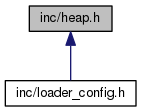
\includegraphics[width=178pt]{heap_8h__dep__incl}
\end{center}
\end{figure}
\subsection*{Data Structures}
\begin{DoxyCompactItemize}
\item 
struct \hyperlink{structheap__stats}{heap\+\_\+stats}
\end{DoxyCompactItemize}
\subsection*{Macros}
\begin{DoxyCompactItemize}
\item 
\#define {\bfseries H\+E\+A\+P\+\_\+\+S\+I\+Z\+E\+\_\+\+B\+Y\+T\+ES}~(256)\hypertarget{heap_8h_af2910747af799b24cfaa2ab32861f592}{}\label{heap_8h_af2910747af799b24cfaa2ab32861f592}

\item 
\#define {\bfseries H\+E\+A\+P\+\_\+\+S\+I\+Z\+E\+\_\+\+W\+O\+R\+DS}~(H\+E\+A\+P\+\_\+\+S\+I\+Z\+E\+\_\+\+B\+Y\+T\+ES / sizeof(int32\+\_\+t))\hypertarget{heap_8h_a08198ef17b67d091f9eb38c544cb4680}{}\label{heap_8h_a08198ef17b67d091f9eb38c544cb4680}

\item 
\#define {\bfseries H\+E\+A\+P\+\_\+\+OK}~0\hypertarget{heap_8h_aa57d61dd0e8d07dce08f6be38001a5ff}{}\label{heap_8h_aa57d61dd0e8d07dce08f6be38001a5ff}

\item 
\#define {\bfseries H\+E\+A\+P\+\_\+\+E\+R\+R\+O\+R\+\_\+\+C\+O\+R\+R\+U\+P\+T\+E\+D\+\_\+\+H\+E\+AP}~1\hypertarget{heap_8h_a4741d1e0f188dbcd4fe46ec0038c59c7}{}\label{heap_8h_a4741d1e0f188dbcd4fe46ec0038c59c7}

\item 
\#define {\bfseries H\+E\+A\+P\+\_\+\+E\+R\+R\+O\+R\+\_\+\+P\+O\+I\+N\+T\+E\+R\+\_\+\+O\+U\+T\+\_\+\+O\+F\+\_\+\+R\+A\+N\+GE}~2\hypertarget{heap_8h_a5400f746fb9c8efb71156c51f766b22e}{}\label{heap_8h_a5400f746fb9c8efb71156c51f766b22e}

\end{DoxyCompactItemize}
\subsection*{Typedefs}
\begin{DoxyCompactItemize}
\item 
typedef struct \hyperlink{structheap__stats}{heap\+\_\+stats} {\bfseries heap\+\_\+stats\+\_\+t}\hypertarget{heap_8h_a286400a036f6f2dc8a3ddca156720932}{}\label{heap_8h_a286400a036f6f2dc8a3ddca156720932}

\end{DoxyCompactItemize}
\subsection*{Functions}
\begin{DoxyCompactItemize}
\item 
int32\+\_\+t \hyperlink{heap_8h_a927f9f9522b87a3ccaee6c68efbf2081}{Heap\+\_\+\+Init} (void)
\begin{DoxyCompactList}\small\item\em Initialize the Heap notes\+: Initializes/resets the heap to a clean state where no memory is allocated. \end{DoxyCompactList}\item 
void $\ast$ \hyperlink{heap_8h_a178556e87b1f3e4c72b419d2c02cd1d4}{Heap\+\_\+\+Malloc} (int32\+\_\+t desired\+Bytes)
\begin{DoxyCompactList}\small\item\em Allocate memory, data not initialized. \end{DoxyCompactList}\item 
void $\ast$ \hyperlink{heap_8h_a2844e924abca6846ed9407e57ed828ab}{Heap\+\_\+\+Calloc} (int32\+\_\+t desired\+Bytes)
\begin{DoxyCompactList}\small\item\em Allocate memory, data are initialized to 0 notes\+: the allocated memory block will be zeroed out. \end{DoxyCompactList}\item 
void $\ast$ \hyperlink{heap_8h_af02282279b1745e0e1485c5bc7d19098}{Heap\+\_\+\+Realloc} (void $\ast$old\+Block, int32\+\_\+t desired\+Bytes)
\begin{DoxyCompactList}\small\item\em Reallocate buffer to a new size notes\+: the given block will be unallocated after its contents are copied to the new block. \end{DoxyCompactList}\item 
int32\+\_\+t \hyperlink{heap_8h_a0c2946e20398909f89ebf1bc344b9f60}{Heap\+\_\+\+Free} (void $\ast$pointer)
\begin{DoxyCompactList}\small\item\em return a block to the heap \end{DoxyCompactList}\item 
int32\+\_\+t \hyperlink{heap_8h_a5c8d75b021d5e6edab5c8e0164224e3e}{Heap\+\_\+\+Test} (void)
\begin{DoxyCompactList}\small\item\em Test the heap. \end{DoxyCompactList}\item 
\hyperlink{structheap__stats}{heap\+\_\+stats\+\_\+t} \hyperlink{heap_8h_a21054e474258ea882ed5765cabaa7c3b}{Heap\+\_\+\+Stats} (void)
\begin{DoxyCompactList}\small\item\em return the current status of the heap \end{DoxyCompactList}\end{DoxyCompactItemize}


\subsection{Detailed Description}
Implements memory heap for dynamic memory allocation. Follows standard malloc/calloc/realloc/free interface for allocating/unallocating memory. modified 8/31/08 Jonathan Valvano for style modified 12/16/11 Jonathan Valvano for 32-\/bit machine modified August 10, 2014 for C99 syntax This example accompanies the book \char`\"{}\+Embedded Systems\+: Real Time Operating Systems for A\+R\+M Cortex M Microcontrollers\char`\"{}, I\+S\+BN\+: 978-\/1466468863, Jonathan Valvano, copyright (c) 2014 Implementation Notes\+: This is a Knuth Heap. Each block has a header and a trailer, which I shall call the meta-\/sections. The meta-\/sections are each a single int32\+\_\+t that tells how many int32\+\_\+ts/words can be stored between the header and trailer. If the block is used, the meta-\/sections record the room as a positive number. If the block is unused, the meta-\/sections record the room as a negative number. Copyright 2014 by Jonathan W. Valvano, \href{mailto:valvano@mail.utexas.edu}{\tt valvano@mail.\+utexas.\+edu} You may use, edit, run or distribute this file as long as the above copyright notice remains T\+H\+IS S\+O\+F\+T\+W\+A\+RE IS P\+R\+O\+V\+I\+D\+ED \char`\"{}\+A\+S I\+S\char`\"{}. NO W\+A\+R\+R\+A\+N\+T\+I\+ES, W\+H\+E\+T\+H\+ER E\+X\+P\+R\+E\+SS, I\+M\+P\+L\+I\+ED OR S\+T\+A\+T\+U\+T\+O\+RY, I\+N\+C\+L\+U\+D\+I\+NG, B\+UT N\+OT L\+I\+M\+I\+T\+ED TO, I\+M\+P\+L\+I\+ED W\+A\+R\+R\+A\+N\+T\+I\+ES OF M\+E\+R\+C\+H\+A\+N\+T\+A\+B\+I\+L\+I\+TY A\+ND F\+I\+T\+N\+E\+SS F\+OR A P\+A\+R\+T\+I\+C\+U\+L\+AR P\+U\+R\+P\+O\+SE A\+P\+P\+LY TO T\+H\+IS S\+O\+F\+T\+W\+A\+RE. V\+A\+L\+V\+A\+NO S\+H\+A\+LL N\+OT, IN A\+NY C\+I\+R\+C\+U\+M\+S\+T\+A\+N\+C\+ES, BE L\+I\+A\+B\+LE F\+OR S\+P\+E\+C\+I\+AL, I\+N\+C\+I\+D\+E\+N\+T\+AL, OR C\+O\+N\+S\+E\+Q\+U\+E\+N\+T\+I\+AL D\+A\+M\+A\+G\+ES, F\+OR A\+NY R\+E\+A\+S\+ON W\+H\+A\+T\+S\+O\+E\+V\+ER. For more information about my classes, my research, and my books, see \href{http://users.ece.utexas.edu/~valvano/}{\tt http\+://users.\+ece.\+utexas.\+edu/$\sim$valvano/}. 

\begin{DoxyAuthor}{Author}
Jacob Egner 
\end{DoxyAuthor}
\begin{DoxyDate}{Date}
2008-\/07-\/31 
\end{DoxyDate}


\subsection{Function Documentation}
\index{heap.\+h@{heap.\+h}!Heap\+\_\+\+Calloc@{Heap\+\_\+\+Calloc}}
\index{Heap\+\_\+\+Calloc@{Heap\+\_\+\+Calloc}!heap.\+h@{heap.\+h}}
\subsubsection[{\texorpdfstring{Heap\+\_\+\+Calloc(int32\+\_\+t desired\+Bytes)}{Heap_Calloc(int32_t desiredBytes)}}]{\setlength{\rightskip}{0pt plus 5cm}void$\ast$ Heap\+\_\+\+Calloc (
\begin{DoxyParamCaption}
\item[{int32\+\_\+t}]{desired\+Bytes}
\end{DoxyParamCaption}
)}\hypertarget{heap_8h_a2844e924abca6846ed9407e57ed828ab}{}\label{heap_8h_a2844e924abca6846ed9407e57ed828ab}


Allocate memory, data are initialized to 0 notes\+: the allocated memory block will be zeroed out. 


\begin{DoxyParams}{Parameters}
{\em desired\+Bytes} & desired number of bytes to allocate\\
\hline
\end{DoxyParams}
\begin{DoxyReturn}{Returns}
void$\ast$ pointing to the allocated memory block or will return N\+U\+LL if there isn\textquotesingle{}t sufficient space to satisfy allocation request 
\end{DoxyReturn}
\index{heap.\+h@{heap.\+h}!Heap\+\_\+\+Free@{Heap\+\_\+\+Free}}
\index{Heap\+\_\+\+Free@{Heap\+\_\+\+Free}!heap.\+h@{heap.\+h}}
\subsubsection[{\texorpdfstring{Heap\+\_\+\+Free(void $\ast$pointer)}{Heap_Free(void *pointer)}}]{\setlength{\rightskip}{0pt plus 5cm}int32\+\_\+t Heap\+\_\+\+Free (
\begin{DoxyParamCaption}
\item[{void $\ast$}]{pointer}
\end{DoxyParamCaption}
)}\hypertarget{heap_8h_a0c2946e20398909f89ebf1bc344b9f60}{}\label{heap_8h_a0c2946e20398909f89ebf1bc344b9f60}


return a block to the heap 


\begin{DoxyParams}{Parameters}
{\em pointer} & the pointer to memory to unallocate\\
\hline
\end{DoxyParams}
\begin{DoxyReturn}{Returns}
H\+E\+A\+P\+\_\+\+OK if everything is ok; H\+E\+A\+P\+\_\+\+E\+R\+R\+O\+R\+\_\+\+P\+O\+I\+N\+T\+E\+R\+\_\+\+O\+U\+T\+\_\+\+O\+F\+\_\+\+R\+A\+N\+GE if pointer points outside the heap; H\+E\+A\+P\+\_\+\+E\+R\+R\+O\+R\+\_\+\+C\+O\+R\+R\+U\+P\+T\+E\+D\+\_\+\+H\+E\+AP if heap has been corrupted or trying to unallocate memory that has already been unallocated; 
\end{DoxyReturn}
\index{heap.\+h@{heap.\+h}!Heap\+\_\+\+Init@{Heap\+\_\+\+Init}}
\index{Heap\+\_\+\+Init@{Heap\+\_\+\+Init}!heap.\+h@{heap.\+h}}
\subsubsection[{\texorpdfstring{Heap\+\_\+\+Init(void)}{Heap_Init(void)}}]{\setlength{\rightskip}{0pt plus 5cm}int32\+\_\+t Heap\+\_\+\+Init (
\begin{DoxyParamCaption}
\item[{void}]{}
\end{DoxyParamCaption}
)}\hypertarget{heap_8h_a927f9f9522b87a3ccaee6c68efbf2081}{}\label{heap_8h_a927f9f9522b87a3ccaee6c68efbf2081}


Initialize the Heap notes\+: Initializes/resets the heap to a clean state where no memory is allocated. 

\begin{DoxyReturn}{Returns}
always H\+E\+A\+P\+\_\+\+OK 
\end{DoxyReturn}
\index{heap.\+h@{heap.\+h}!Heap\+\_\+\+Malloc@{Heap\+\_\+\+Malloc}}
\index{Heap\+\_\+\+Malloc@{Heap\+\_\+\+Malloc}!heap.\+h@{heap.\+h}}
\subsubsection[{\texorpdfstring{Heap\+\_\+\+Malloc(int32\+\_\+t desired\+Bytes)}{Heap_Malloc(int32_t desiredBytes)}}]{\setlength{\rightskip}{0pt plus 5cm}void$\ast$ Heap\+\_\+\+Malloc (
\begin{DoxyParamCaption}
\item[{int32\+\_\+t}]{desired\+Bytes}
\end{DoxyParamCaption}
)}\hypertarget{heap_8h_a178556e87b1f3e4c72b419d2c02cd1d4}{}\label{heap_8h_a178556e87b1f3e4c72b419d2c02cd1d4}


Allocate memory, data not initialized. 


\begin{DoxyParams}{Parameters}
{\em desired\+Bytes} & desired number of bytes to allocate\\
\hline
\end{DoxyParams}
\begin{DoxyReturn}{Returns}
void$\ast$ pointing to the allocated memory or will return N\+U\+LL if there isn\textquotesingle{}t sufficient space to satisfy allocation request 
\end{DoxyReturn}
\index{heap.\+h@{heap.\+h}!Heap\+\_\+\+Realloc@{Heap\+\_\+\+Realloc}}
\index{Heap\+\_\+\+Realloc@{Heap\+\_\+\+Realloc}!heap.\+h@{heap.\+h}}
\subsubsection[{\texorpdfstring{Heap\+\_\+\+Realloc(void $\ast$old\+Block, int32\+\_\+t desired\+Bytes)}{Heap_Realloc(void *oldBlock, int32_t desiredBytes)}}]{\setlength{\rightskip}{0pt plus 5cm}void$\ast$ Heap\+\_\+\+Realloc (
\begin{DoxyParamCaption}
\item[{void $\ast$}]{old\+Block, }
\item[{int32\+\_\+t}]{desired\+Bytes}
\end{DoxyParamCaption}
)}\hypertarget{heap_8h_af02282279b1745e0e1485c5bc7d19098}{}\label{heap_8h_af02282279b1745e0e1485c5bc7d19098}


Reallocate buffer to a new size notes\+: the given block will be unallocated after its contents are copied to the new block. 


\begin{DoxyParams}{Parameters}
{\em old\+Block} & pointer to a block\\
\hline
{\em desired\+Bytes} & a desired number of bytes for a new block where the contents of the old block will be copied to\\
\hline
\end{DoxyParams}
\begin{DoxyReturn}{Returns}
void$\ast$ pointing to the new block or will return N\+U\+LL if there is any reason the reallocation can\textquotesingle{}t be completed 
\end{DoxyReturn}
\index{heap.\+h@{heap.\+h}!Heap\+\_\+\+Stats@{Heap\+\_\+\+Stats}}
\index{Heap\+\_\+\+Stats@{Heap\+\_\+\+Stats}!heap.\+h@{heap.\+h}}
\subsubsection[{\texorpdfstring{Heap\+\_\+\+Stats(void)}{Heap_Stats(void)}}]{\setlength{\rightskip}{0pt plus 5cm}{\bf heap\+\_\+stats\+\_\+t} Heap\+\_\+\+Stats (
\begin{DoxyParamCaption}
\item[{void}]{}
\end{DoxyParamCaption}
)}\hypertarget{heap_8h_a21054e474258ea882ed5765cabaa7c3b}{}\label{heap_8h_a21054e474258ea882ed5765cabaa7c3b}


return the current status of the heap 

\begin{DoxyReturn}{Returns}
a heap\+\_\+stats\+\_\+t that describes the current usage of the heap 
\end{DoxyReturn}
\index{heap.\+h@{heap.\+h}!Heap\+\_\+\+Test@{Heap\+\_\+\+Test}}
\index{Heap\+\_\+\+Test@{Heap\+\_\+\+Test}!heap.\+h@{heap.\+h}}
\subsubsection[{\texorpdfstring{Heap\+\_\+\+Test(void)}{Heap_Test(void)}}]{\setlength{\rightskip}{0pt plus 5cm}int32\+\_\+t Heap\+\_\+\+Test (
\begin{DoxyParamCaption}
\item[{void}]{}
\end{DoxyParamCaption}
)}\hypertarget{heap_8h_a5c8d75b021d5e6edab5c8e0164224e3e}{}\label{heap_8h_a5c8d75b021d5e6edab5c8e0164224e3e}


Test the heap. 

\begin{DoxyReturn}{Returns}
validity of the heap -\/ either H\+E\+A\+P\+\_\+\+OK or H\+E\+A\+P\+\_\+\+E\+R\+R\+O\+R\+\_\+\+H\+E\+A\+P\+\_\+\+C\+O\+R\+R\+U\+P\+T\+ED 
\end{DoxyReturn}

\hypertarget{interpreter_8h}{}\section{inc/interpreter.h File Reference}
\label{interpreter_8h}\index{inc/interpreter.\+h@{inc/interpreter.\+h}}
\subsection*{Functions}
\begin{DoxyCompactItemize}
\item 
void \hyperlink{interpreter_8h_a0cf6f7b20306bd53e7f61b3ead179154}{interpreter\+\_\+task} (void)\hypertarget{interpreter_8h_a0cf6f7b20306bd53e7f61b3ead179154}{}\label{interpreter_8h_a0cf6f7b20306bd53e7f61b3ead179154}

\begin{DoxyCompactList}\small\item\em OS Task that sends characters to the interpreter. \end{DoxyCompactList}\item 
void \hyperlink{interpreter_8h_ad36afca5c99ec60b995fae704d95d014}{interpreter\+\_\+cmd} (char $\ast$cmd\+\_\+str)
\begin{DoxyCompactList}\small\item\em Pass user input to the interpreter and act on their command. \end{DoxyCompactList}\end{DoxyCompactItemize}


\subsection{Detailed Description}
List of commands
\begin{DoxyItemize}
\item adc
\begin{DoxyItemize}
\item Prints 2 consecutive A\+DC samples of channel 0 to the L\+CD and U\+A\+R\+T0
\end{DoxyItemize}
\item lcd
\begin{DoxyItemize}
\item Prints strings on each line of each logical display on the L\+CD.
\end{DoxyItemize}
\item critical
\begin{DoxyItemize}
\item Prints the percentage of C\+PU time spent with interrupts disabled.
\end{DoxyItemize}
\item log
\begin{DoxyItemize}
\item Prints profiler events logged
\end{DoxyItemize}
\item clear
\begin{DoxyItemize}
\item Clears the profiler event log and restarts the profiler
\end{DoxyItemize}
\item format
\begin{DoxyItemize}
\item Formats the filesystem on the SD card
\end{DoxyItemize}
\item ls
\begin{DoxyItemize}
\item List all files in the filesystem
\end{DoxyItemize}
\item cat
\begin{DoxyItemize}
\item Print out file in the filesystem.
\item Takes one argument\+: the name of the file to print
\end{DoxyItemize}
\item rm
\begin{DoxyItemize}
\item Remove file in the filesystem.
\item Takes one argument\+: the name of the file to remove
\end{DoxyItemize}
\item touch
\begin{DoxyItemize}
\item Create a file in the filesystem.
\item Takes one argument\+: the name of the file to create
\end{DoxyItemize}
\item echo
\begin{DoxyItemize}
\item Append characters to a file
\item Takes two arguments in this order\+:
\begin{DoxyItemize}
\item The name of the file to append to
\item Remaining characters are written to the file
\end{DoxyItemize}
\end{DoxyItemize}
\item increase
\begin{DoxyItemize}
\item Artificially increase the time spent in critical sections to test the \char`\"{}critical\char`\"{} command. 
\end{DoxyItemize}
\end{DoxyItemize}

\subsection{Function Documentation}
\index{interpreter.\+h@{interpreter.\+h}!interpreter\+\_\+cmd@{interpreter\+\_\+cmd}}
\index{interpreter\+\_\+cmd@{interpreter\+\_\+cmd}!interpreter.\+h@{interpreter.\+h}}
\subsubsection[{\texorpdfstring{interpreter\+\_\+cmd(char $\ast$cmd\+\_\+str)}{interpreter_cmd(char *cmd_str)}}]{\setlength{\rightskip}{0pt plus 5cm}void interpreter\+\_\+cmd (
\begin{DoxyParamCaption}
\item[{char $\ast$}]{cmd\+\_\+str}
\end{DoxyParamCaption}
)}\hypertarget{interpreter_8h_ad36afca5c99ec60b995fae704d95d014}{}\label{interpreter_8h_ad36afca5c99ec60b995fae704d95d014}


Pass user input to the interpreter and act on their command. 


\begin{DoxyParams}{Parameters}
{\em cmd\+\_\+str} & String containing the entire user command. \\
\hline
\end{DoxyParams}

\hypertarget{misc__macros_8h}{}\section{inc/misc\+\_\+macros.h File Reference}
\label{misc__macros_8h}\index{inc/misc\+\_\+macros.\+h@{inc/misc\+\_\+macros.\+h}}


Some helper macros.  


\subsection*{Macros}
\begin{DoxyCompactItemize}
\item 
\#define \hyperlink{misc__macros_8h_ad53b2827d15d4f100433764eea395a94}{lengthof}(array)~(sizeof(array)/sizeof((array)\mbox{[}0\mbox{]}))\hypertarget{misc__macros_8h_ad53b2827d15d4f100433764eea395a94}{}\label{misc__macros_8h_ad53b2827d15d4f100433764eea395a94}

\begin{DoxyCompactList}\small\item\em Get the number of elements in an array. \end{DoxyCompactList}\item 
\#define \hyperlink{misc__macros_8h_a06311b356862bfe3ac93fedc89c5c066}{zeroes}(array)~memset(array, 0, sizeof(array))\hypertarget{misc__macros_8h_a06311b356862bfe3ac93fedc89c5c066}{}\label{misc__macros_8h_a06311b356862bfe3ac93fedc89c5c066}

\begin{DoxyCompactList}\small\item\em Zeroes out an array. \end{DoxyCompactList}\end{DoxyCompactItemize}


\subsection{Detailed Description}
Some helper macros. 


\hypertarget{OS_8h}{}\section{inc/\+OS.h File Reference}
\label{OS_8h}\index{inc/\+O\+S.\+h@{inc/\+O\+S.\+h}}


Real Time Operating System for Labs 2 and 3 E\+E445\+M/\+E\+E380\+L.\+12.  


{\ttfamily \#include $<$stdint.\+h$>$}\\*
Include dependency graph for O\+S.\+h\+:\nopagebreak
\begin{figure}[H]
\begin{center}
\leavevmode
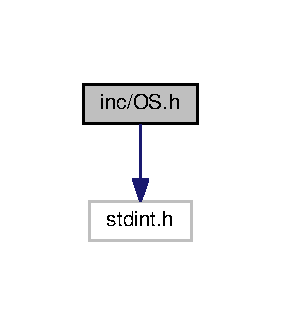
\includegraphics[width=135pt]{OS_8h__incl}
\end{center}
\end{figure}
This graph shows which files directly or indirectly include this file\+:\nopagebreak
\begin{figure}[H]
\begin{center}
\leavevmode
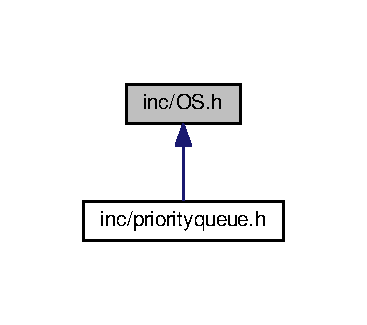
\includegraphics[width=176pt]{OS_8h__dep__incl}
\end{center}
\end{figure}
\subsection*{Data Structures}
\begin{DoxyCompactItemize}
\item 
struct \hyperlink{struct__pcb__s}{\+\_\+pcb\+\_\+s}
\item 
struct \hyperlink{struct__tcb__s}{\+\_\+tcb\+\_\+s}
\item 
struct \hyperlink{structSema4}{Sema4}
\end{DoxyCompactItemize}
\subsection*{Macros}
\begin{DoxyCompactItemize}
\item 
\#define {\bfseries T\+I\+M\+E\+\_\+1\+MS}~80000\hypertarget{OS_8h_ad6445469b3084b0c8a8ea272e8a40a17}{}\label{OS_8h_ad6445469b3084b0c8a8ea272e8a40a17}

\item 
\#define {\bfseries T\+I\+M\+E\+\_\+2\+MS}~(2 $\ast$ T\+I\+M\+E\+\_\+1\+MS)\hypertarget{OS_8h_a601fb0d91385070bae69c2b1c4e63162}{}\label{OS_8h_a601fb0d91385070bae69c2b1c4e63162}

\item 
\#define {\bfseries T\+I\+M\+E\+\_\+500\+US}~(T\+I\+M\+E\+\_\+1\+MS / 2)\hypertarget{OS_8h_a5bd8a6024a3e7cd43b7fe30988ca81e8}{}\label{OS_8h_a5bd8a6024a3e7cd43b7fe30988ca81e8}

\item 
\#define {\bfseries T\+I\+M\+E\+\_\+250\+US}~(T\+I\+M\+E\+\_\+1\+MS / 4)\hypertarget{OS_8h_aae4936d8a1bad649da44cacada40b157}{}\label{OS_8h_aae4936d8a1bad649da44cacada40b157}

\item 
\#define {\bfseries T\+A\+S\+K\+\_\+\+S\+T\+A\+C\+K\+\_\+\+S\+I\+ZE}~128\hypertarget{OS_8h_a5486258f1f34d3baeda92a74b63c27c3}{}\label{OS_8h_a5486258f1f34d3baeda92a74b63c27c3}

\item 
\#define {\bfseries T\+C\+B\+\_\+\+M\+A\+G\+IC}~(0x900d900d)\hypertarget{OS_8h_a0fb8aa2f0ea0a6494f1639dd97087013}{}\label{OS_8h_a0fb8aa2f0ea0a6494f1639dd97087013}

\item 
\#define \hyperlink{OS_8h_accb79b9446dd2b953a1fb8437c5f6e15}{O\+S\+\_\+\+Add\+Thread}(task,  stack\+Size,  priority)
\item 
\#define \hyperlink{OS_8h_adf56561acbee98b34e8c42ff6b147255}{O\+S\+\_\+\+Add\+Periodic\+Thread}(task,  period,  priority)~O\+S\+\_\+\+Add\+Periodic\+Thread\+\_\+priv(task, period, priority, \#task)
\end{DoxyCompactItemize}
\subsection*{Typedefs}
\begin{DoxyCompactItemize}
\item 
typedef struct \hyperlink{struct__pcb__s}{\+\_\+pcb\+\_\+s} {\bfseries pcb\+\_\+t}\hypertarget{OS_8h_add17966847109f7551977a87ddfcd8aa}{}\label{OS_8h_add17966847109f7551977a87ddfcd8aa}

\item 
typedef struct \hyperlink{struct__tcb__s}{\+\_\+tcb\+\_\+s} {\bfseries tcb\+\_\+t}\hypertarget{OS_8h_a5f5b511a2a589828581399459da62c6a}{}\label{OS_8h_a5f5b511a2a589828581399459da62c6a}

\item 
typedef struct \hyperlink{structSema4}{Sema4} {\bfseries Sema4\+Type}\hypertarget{OS_8h_a798fbe37dbc49a5ff9af51bf7de1ee8e}{}\label{OS_8h_a798fbe37dbc49a5ff9af51bf7de1ee8e}

\end{DoxyCompactItemize}
\subsection*{Functions}
\begin{DoxyCompactItemize}
\item 
void \hyperlink{OS_8h_acb6df8f47f418aad9c9a9e045d7d1e6d}{O\+S\+\_\+\+Init} (void)
\item 
void \hyperlink{OS_8h_af580c6222330cc3d214763ddac7800b9}{O\+S\+\_\+\+Init\+Semaphore} (\hyperlink{structSema4}{Sema4\+Type} $\ast$sema\+Pt, long value)
\item 
void \hyperlink{OS_8h_aad29612829941c857ed685f40e193cd0}{O\+S\+\_\+\+Wait} (\hyperlink{structSema4}{Sema4\+Type} $\ast$sema\+Pt)
\item 
void \hyperlink{OS_8h_a0c4d587c411a23652529110910261fde}{O\+S\+\_\+\+Signal} (\hyperlink{structSema4}{Sema4\+Type} $\ast$sema\+Pt)
\item 
void \hyperlink{OS_8h_a3f127f7a40ffd3e43b7b0f4c8b7f30ff}{O\+S\+\_\+b\+Wait} (\hyperlink{structSema4}{Sema4\+Type} $\ast$sema\+Pt)
\item 
void \hyperlink{OS_8h_aacf0c377b570fc63b103c57e0fbc7acd}{O\+S\+\_\+b\+Signal} (\hyperlink{structSema4}{Sema4\+Type} $\ast$sema\+Pt)
\item 
void \hyperlink{OS_8h_a075cf7301361417f66be1d5c22e36b0f}{Jitter} (void)\hypertarget{OS_8h_a075cf7301361417f66be1d5c22e36b0f}{}\label{OS_8h_a075cf7301361417f66be1d5c22e36b0f}

\begin{DoxyCompactList}\small\item\em Print the max periodic task jitter measured thus far to the S\+T7735 display. \end{DoxyCompactList}\item 
int {\bfseries \+\_\+\+\_\+\+O\+S\+\_\+\+Add\+Thread} (void($\ast$task)(void), unsigned long stack\+Size, unsigned long priority, char $\ast$task\+\_\+name, \hyperlink{struct__pcb__s}{pcb\+\_\+t} $\ast$parent\+\_\+process)\hypertarget{OS_8h_a3e5c42edf8d08a40ccdee09e200d84b6}{}\label{OS_8h_a3e5c42edf8d08a40ccdee09e200d84b6}

\item 
unsigned long \hyperlink{OS_8h_adc21b8aab03cbb1611186ca3ac9123d8}{O\+S\+\_\+\+Id} (void)
\item 
int {\bfseries O\+S\+\_\+\+Add\+Periodic\+Thread\+\_\+priv} (void($\ast$task)(void), unsigned long period, unsigned long priority, char $\ast$task\+\_\+name)\hypertarget{OS_8h_a21ee017683a4a2b593d5497a27addac0}{}\label{OS_8h_a21ee017683a4a2b593d5497a27addac0}

\item 
int \hyperlink{OS_8h_a5c387e683842fc4f9f846729a60186da}{O\+S\+\_\+\+Add\+S\+W1\+Task} (void($\ast$task)(void), unsigned long priority)
\item 
int \hyperlink{OS_8h_a508ed7f6202df8a9e500994ad4399784}{O\+S\+\_\+\+Add\+S\+W2\+Task} (void($\ast$task)(void), unsigned long priority)
\item 
void \hyperlink{OS_8h_aeeb2aca9e1a16738a5d82353b2d497ac}{O\+S\+\_\+\+Sleep} (unsigned long sleep\+Time)
\item 
void \hyperlink{OS_8h_a8e991f4f2576c5cfec04ef5f37aabea5}{O\+S\+\_\+\+Kill} (void)
\item 
void \hyperlink{OS_8h_a4e71587568a2a48931a35615cad1b5db}{O\+S\+\_\+\+Suspend} (void)
\item 
void \hyperlink{OS_8h_a361ff1137f5dad8e0a74631be6fb12b6}{O\+S\+\_\+\+Fifo\+\_\+\+Init} (unsigned long size)
\item 
int \hyperlink{OS_8h_adf231073602c9328f6248f6272d63e7f}{O\+S\+\_\+\+Fifo\+\_\+\+Put} (unsigned long data)
\item 
unsigned long \hyperlink{OS_8h_af899a42296039e22ffdd8bf6e1ca208e}{O\+S\+\_\+\+Fifo\+\_\+\+Get} (void)
\item 
long \hyperlink{OS_8h_a9ff4cb899801f20ff90cbf2717c154c7}{O\+S\+\_\+\+Fifo\+\_\+\+Size} (void)
\item 
void \hyperlink{OS_8h_a84e1a933dd73e319fdd5649c2270281b}{O\+S\+\_\+\+Mail\+Box\+\_\+\+Init} (void)
\item 
void \hyperlink{OS_8h_ac4c3ebdb61c0c11195d6fcafeb0d4c99}{O\+S\+\_\+\+Mail\+Box\+\_\+\+Send} (unsigned long data)
\item 
unsigned long \hyperlink{OS_8h_ace71083584f0f1e5e2f081f1e4a1394a}{O\+S\+\_\+\+Mail\+Box\+\_\+\+Recv} (void)
\item 
unsigned long long \hyperlink{OS_8h_a5798d7fa05a4c3a523efe1b5651c5318}{O\+S\+\_\+\+Time} (void)
\item 
unsigned long long \hyperlink{OS_8h_af4b27f93116607bd3986125cb1c9edcf}{O\+S\+\_\+\+Time\+Difference} (unsigned long long start, unsigned long long stop)
\item 
void \hyperlink{OS_8h_ace6ec4b7947542f7d7ff3104d8c759bd}{O\+S\+\_\+\+Clear\+Ms\+Time} (void)
\item 
unsigned long \hyperlink{OS_8h_a251073790d2782617fd7474625761573}{O\+S\+\_\+\+Ms\+Time} (void)
\item 
void \hyperlink{OS_8h_a18553a7e1d82dcaaeb80a5524bd01cf2}{O\+S\+\_\+\+Launch} (unsigned long the\+Time\+Slice)
\item 
int \hyperlink{OS_8h_a3271236396a143a19c9650377e0f32ee}{O\+S\+\_\+\+Add\+Process} (void($\ast$entry)(void), void $\ast$text, void $\ast$data, unsigned long stack\+Size, unsigned long priority)
\begin{DoxyCompactList}\small\item\em Launch a process in the OS. \end{DoxyCompactList}\item 
long {\bfseries Start\+Critical} (void)\hypertarget{OS_8h_a6e7e2088607214bc15b17ac57b57df1b}{}\label{OS_8h_a6e7e2088607214bc15b17ac57b57df1b}

\item 
void {\bfseries End\+Critical} (long sr)\hypertarget{OS_8h_a670da3ff1aea0c7d54c40e9e40b5eeed}{}\label{OS_8h_a670da3ff1aea0c7d54c40e9e40b5eeed}

\item 
void {\bfseries Disable\+Interrupts} (void)\hypertarget{OS_8h_ac866dbaf7b167e5c46bb33de42eee84d}{}\label{OS_8h_ac866dbaf7b167e5c46bb33de42eee84d}

\item 
void {\bfseries Enable\+Interrupts} (void)\hypertarget{OS_8h_ab712356331a62b04aebcb373865e68c4}{}\label{OS_8h_ab712356331a62b04aebcb373865e68c4}

\end{DoxyCompactItemize}
\subsection*{Variables}
\begin{DoxyCompactItemize}
\item 
\hyperlink{struct__tcb__s}{tcb\+\_\+t} $\ast$ {\bfseries cur\+\_\+tcb}\hypertarget{OS_8h_aa1c72d659051f84119a2c6373fe43bee}{}\label{OS_8h_aa1c72d659051f84119a2c6373fe43bee}

\end{DoxyCompactItemize}


\subsection{Detailed Description}
Real Time Operating System for Labs 2 and 3 E\+E445\+M/\+E\+E380\+L.\+12. 

R\+T\+OS kernel capable of round-\/robin scheduling, up to 2 low-\/jitter periodic tasks.

Reserves W\+T\+I\+M\+E\+R1A and B for periodic task scheduling. Reserves Sys\+Tick timer for round-\/robin scheduling. Reserves W\+T\+I\+M\+E\+R0 as a 64-\/bit time source.

Interface by Jonathan W. Valvano 2/20/17, \href{mailto:valvano@mail.utexas.edu}{\tt valvano@mail.\+utexas.\+edu} Implementation by Riley Wood and Jeageun Jung \begin{DoxyAuthor}{Author}
Riley Wood and Jeageun Jung 
\end{DoxyAuthor}


\subsection{Macro Definition Documentation}
\index{O\+S.\+h@{O\+S.\+h}!O\+S\+\_\+\+Add\+Periodic\+Thread@{O\+S\+\_\+\+Add\+Periodic\+Thread}}
\index{O\+S\+\_\+\+Add\+Periodic\+Thread@{O\+S\+\_\+\+Add\+Periodic\+Thread}!O\+S.\+h@{O\+S.\+h}}
\subsubsection[{\texorpdfstring{O\+S\+\_\+\+Add\+Periodic\+Thread}{OS_AddPeriodicThread}}]{\setlength{\rightskip}{0pt plus 5cm}\#define O\+S\+\_\+\+Add\+Periodic\+Thread(
\begin{DoxyParamCaption}
\item[{}]{task, }
\item[{}]{period, }
\item[{}]{priority}
\end{DoxyParamCaption}
)~O\+S\+\_\+\+Add\+Periodic\+Thread\+\_\+priv(task, period, priority, \#task)}\hypertarget{OS_8h_adf56561acbee98b34e8c42ff6b147255}{}\label{OS_8h_adf56561acbee98b34e8c42ff6b147255}
Add a background periodic task. Typically this function receives the highest priority You are free to select the time resolution for this function It is assumed that the user task will run to completion and return This task can not spin, block, loop, sleep, or kill This task can call O\+S\+\_\+\+Signal O\+S\+\_\+b\+Signal O\+S\+\_\+\+Add\+Thread This task does not have a Thread ID In lab 2, this command will be called 0 or 1 times In lab 2, the priority field can be ignored In lab 3, this command will be called 0 1 or 2 times In lab 3, there will be up to four background threads, and this priority field determines the relative priority of these four threads 
\begin{DoxyParams}{Parameters}
{\em task} & pointer to a void/void background function \\
\hline
{\em period} & given in system time units (12.\+5ns) \\
\hline
{\em priority} & 0 is the highest, 5 is the lowest \\
\hline
\end{DoxyParams}
\begin{DoxyReturn}{Returns}
1 if successful, 0 if this thread can not be added 
\end{DoxyReturn}
\index{O\+S.\+h@{O\+S.\+h}!O\+S\+\_\+\+Add\+Thread@{O\+S\+\_\+\+Add\+Thread}}
\index{O\+S\+\_\+\+Add\+Thread@{O\+S\+\_\+\+Add\+Thread}!O\+S.\+h@{O\+S.\+h}}
\subsubsection[{\texorpdfstring{O\+S\+\_\+\+Add\+Thread}{OS_AddThread}}]{\setlength{\rightskip}{0pt plus 5cm}\#define O\+S\+\_\+\+Add\+Thread(
\begin{DoxyParamCaption}
\item[{}]{task, }
\item[{}]{stack\+Size, }
\item[{}]{priority}
\end{DoxyParamCaption}
)}\hypertarget{OS_8h_accb79b9446dd2b953a1fb8437c5f6e15}{}\label{OS_8h_accb79b9446dd2b953a1fb8437c5f6e15}
{\bfseries Value\+:}
\begin{DoxyCode}
\_\_OS\_AddThread(task,\(\backslash\)
                                                               stackSize,\(\backslash\)
                                                               priority,\(\backslash\)
                                                               #task,\(\backslash\)
                                                               cur\_tcb ? cur\_tcb->parent\_process : 0)
\end{DoxyCode}
add a foregound thread to the scheduler stack size must be divisable by 8 (aligned to double word boundary) In Lab 2, you can ignore both the stack\+Size and priority fields In Lab 3, you can ignore the stack\+Size fields 
\begin{DoxyParams}{Parameters}
{\em task} & Task function \\
\hline
{\em stack\+Size} & Size of the stack in bytes. Should be divisible by 8 \\
\hline
{\em priority} & Priority of the task. 0 is highest, 5 is lowest. \\
\hline
\end{DoxyParams}
\begin{DoxyReturn}{Returns}
1 if successful, 0 if this thread can not be added 
\end{DoxyReturn}


\subsection{Function Documentation}
\index{O\+S.\+h@{O\+S.\+h}!O\+S\+\_\+\+Add\+Process@{O\+S\+\_\+\+Add\+Process}}
\index{O\+S\+\_\+\+Add\+Process@{O\+S\+\_\+\+Add\+Process}!O\+S.\+h@{O\+S.\+h}}
\subsubsection[{\texorpdfstring{O\+S\+\_\+\+Add\+Process(void($\ast$entry)(void), void $\ast$text, void $\ast$data, unsigned long stack\+Size, unsigned long priority)}{OS_AddProcess(void(*entry)(void), void *text, void *data, unsigned long stackSize, unsigned long priority)}}]{\setlength{\rightskip}{0pt plus 5cm}int O\+S\+\_\+\+Add\+Process (
\begin{DoxyParamCaption}
\item[{void($\ast$)(void)}]{entry, }
\item[{void $\ast$}]{text, }
\item[{void $\ast$}]{data, }
\item[{unsigned long}]{stack\+Size, }
\item[{unsigned long}]{priority}
\end{DoxyParamCaption}
)}\hypertarget{OS_8h_a3271236396a143a19c9650377e0f32ee}{}\label{OS_8h_a3271236396a143a19c9650377e0f32ee}


Launch a process in the OS. 


\begin{DoxyParams}{Parameters}
{\em entry} & Entry point, usually main() of the process \\
\hline
{\em text} & Text (code) section start address \\
\hline
{\em data} & Data section start address \\
\hline
{\em stack\+Size} & Size of the stack for the first thread \\
\hline
{\em priority} & Priority for the first thread \\
\hline
\end{DoxyParams}
\begin{DoxyReturn}{Returns}
int 0 on success, -\/1 on failure. 
\end{DoxyReturn}
\index{O\+S.\+h@{O\+S.\+h}!O\+S\+\_\+\+Add\+S\+W1\+Task@{O\+S\+\_\+\+Add\+S\+W1\+Task}}
\index{O\+S\+\_\+\+Add\+S\+W1\+Task@{O\+S\+\_\+\+Add\+S\+W1\+Task}!O\+S.\+h@{O\+S.\+h}}
\subsubsection[{\texorpdfstring{O\+S\+\_\+\+Add\+S\+W1\+Task(void($\ast$task)(void), unsigned long priority)}{OS_AddSW1Task(void(*task)(void), unsigned long priority)}}]{\setlength{\rightskip}{0pt plus 5cm}int O\+S\+\_\+\+Add\+S\+W1\+Task (
\begin{DoxyParamCaption}
\item[{void($\ast$)(void)}]{task, }
\item[{unsigned long}]{priority}
\end{DoxyParamCaption}
)}\hypertarget{OS_8h_a5c387e683842fc4f9f846729a60186da}{}\label{OS_8h_a5c387e683842fc4f9f846729a60186da}
add a background task to run whenever the S\+W1 (P\+F4) button is pushed 
\begin{DoxyParams}{Parameters}
{\em pointer} & to a void/void background function \\
\hline
{\em priority} & 0 is the highest, 5 is the lowest \\
\hline
\end{DoxyParams}
\begin{DoxyReturn}{Returns}
1 if successful, 0 if this thread can not be added It is assumed that the user task will run to completion and return This task can not spin, block, loop, sleep, or kill This task can call O\+S\+\_\+\+Signal O\+S\+\_\+b\+Signal O\+S\+\_\+\+Add\+Thread This task does not have a Thread ID In labs 2 and 3, this command will be called 0 or 1 times In lab 2, the priority field can be ignored In lab 3, there will be up to four background threads, and this priority field determines the relative priority of these four threads 
\end{DoxyReturn}
\index{O\+S.\+h@{O\+S.\+h}!O\+S\+\_\+\+Add\+S\+W2\+Task@{O\+S\+\_\+\+Add\+S\+W2\+Task}}
\index{O\+S\+\_\+\+Add\+S\+W2\+Task@{O\+S\+\_\+\+Add\+S\+W2\+Task}!O\+S.\+h@{O\+S.\+h}}
\subsubsection[{\texorpdfstring{O\+S\+\_\+\+Add\+S\+W2\+Task(void($\ast$task)(void), unsigned long priority)}{OS_AddSW2Task(void(*task)(void), unsigned long priority)}}]{\setlength{\rightskip}{0pt plus 5cm}int O\+S\+\_\+\+Add\+S\+W2\+Task (
\begin{DoxyParamCaption}
\item[{void($\ast$)(void)}]{task, }
\item[{unsigned long}]{priority}
\end{DoxyParamCaption}
)}\hypertarget{OS_8h_a508ed7f6202df8a9e500994ad4399784}{}\label{OS_8h_a508ed7f6202df8a9e500994ad4399784}
add a background task to run whenever the S\+W2 (P\+F0) button is pushed 
\begin{DoxyParams}{Parameters}
{\em pointer} & to a void/void background function \\
\hline
{\em priority} & 0 is highest, 5 is lowest \\
\hline
\end{DoxyParams}
\begin{DoxyReturn}{Returns}
1 if successful, 0 if this thread can not be added It is assumed user task will run to completion and return This task can not spin block loop sleep or kill This task can call issue O\+S\+\_\+\+Signal, it can call O\+S\+\_\+\+Add\+Thread This task does not have a Thread ID In lab 2, this function can be ignored In lab 3, this command will be called will be called 0 or 1 times In lab 3, there will be up to four background threads, and this priority field determines the relative priority of these four threads 
\end{DoxyReturn}
\index{O\+S.\+h@{O\+S.\+h}!O\+S\+\_\+b\+Signal@{O\+S\+\_\+b\+Signal}}
\index{O\+S\+\_\+b\+Signal@{O\+S\+\_\+b\+Signal}!O\+S.\+h@{O\+S.\+h}}
\subsubsection[{\texorpdfstring{O\+S\+\_\+b\+Signal(\+Sema4\+Type $\ast$sema\+Pt)}{OS_bSignal(Sema4Type *semaPt)}}]{\setlength{\rightskip}{0pt plus 5cm}void O\+S\+\_\+b\+Signal (
\begin{DoxyParamCaption}
\item[{{\bf Sema4\+Type} $\ast$}]{sema\+Pt}
\end{DoxyParamCaption}
)}\hypertarget{OS_8h_aacf0c377b570fc63b103c57e0fbc7acd}{}\label{OS_8h_aacf0c377b570fc63b103c57e0fbc7acd}
Lab2 spinlock, set to 1 Lab3 wakeup blocked thread if appropriate 
\begin{DoxyParams}{Parameters}
{\em sema\+Pt} & pointer to a binary semaphore \\
\hline
\end{DoxyParams}
\index{O\+S.\+h@{O\+S.\+h}!O\+S\+\_\+b\+Wait@{O\+S\+\_\+b\+Wait}}
\index{O\+S\+\_\+b\+Wait@{O\+S\+\_\+b\+Wait}!O\+S.\+h@{O\+S.\+h}}
\subsubsection[{\texorpdfstring{O\+S\+\_\+b\+Wait(\+Sema4\+Type $\ast$sema\+Pt)}{OS_bWait(Sema4Type *semaPt)}}]{\setlength{\rightskip}{0pt plus 5cm}void O\+S\+\_\+b\+Wait (
\begin{DoxyParamCaption}
\item[{{\bf Sema4\+Type} $\ast$}]{sema\+Pt}
\end{DoxyParamCaption}
)}\hypertarget{OS_8h_a3f127f7a40ffd3e43b7b0f4c8b7f30ff}{}\label{OS_8h_a3f127f7a40ffd3e43b7b0f4c8b7f30ff}
Lab2 spinlock, set to 0 Lab3 block if less than zero 
\begin{DoxyParams}{Parameters}
{\em sema\+Pt} & pointer to a binary semaphore \\
\hline
\end{DoxyParams}
\index{O\+S.\+h@{O\+S.\+h}!O\+S\+\_\+\+Clear\+Ms\+Time@{O\+S\+\_\+\+Clear\+Ms\+Time}}
\index{O\+S\+\_\+\+Clear\+Ms\+Time@{O\+S\+\_\+\+Clear\+Ms\+Time}!O\+S.\+h@{O\+S.\+h}}
\subsubsection[{\texorpdfstring{O\+S\+\_\+\+Clear\+Ms\+Time(void)}{OS_ClearMsTime(void)}}]{\setlength{\rightskip}{0pt plus 5cm}void O\+S\+\_\+\+Clear\+Ms\+Time (
\begin{DoxyParamCaption}
\item[{void}]{}
\end{DoxyParamCaption}
)}\hypertarget{OS_8h_ace6ec4b7947542f7d7ff3104d8c759bd}{}\label{OS_8h_ace6ec4b7947542f7d7ff3104d8c759bd}
Sets the system time to zero (from Lab 1). You are free to change how this works. \begin{DoxyReturn}{Returns}
none 
\end{DoxyReturn}
\index{O\+S.\+h@{O\+S.\+h}!O\+S\+\_\+\+Fifo\+\_\+\+Get@{O\+S\+\_\+\+Fifo\+\_\+\+Get}}
\index{O\+S\+\_\+\+Fifo\+\_\+\+Get@{O\+S\+\_\+\+Fifo\+\_\+\+Get}!O\+S.\+h@{O\+S.\+h}}
\subsubsection[{\texorpdfstring{O\+S\+\_\+\+Fifo\+\_\+\+Get(void)}{OS_Fifo_Get(void)}}]{\setlength{\rightskip}{0pt plus 5cm}unsigned long O\+S\+\_\+\+Fifo\+\_\+\+Get (
\begin{DoxyParamCaption}
\item[{void}]{}
\end{DoxyParamCaption}
)}\hypertarget{OS_8h_af899a42296039e22ffdd8bf6e1ca208e}{}\label{OS_8h_af899a42296039e22ffdd8bf6e1ca208e}
Remove one data sample from the Fifo. Called in foreground, will spin/block if empty \begin{DoxyReturn}{Returns}
data 
\end{DoxyReturn}
\index{O\+S.\+h@{O\+S.\+h}!O\+S\+\_\+\+Fifo\+\_\+\+Init@{O\+S\+\_\+\+Fifo\+\_\+\+Init}}
\index{O\+S\+\_\+\+Fifo\+\_\+\+Init@{O\+S\+\_\+\+Fifo\+\_\+\+Init}!O\+S.\+h@{O\+S.\+h}}
\subsubsection[{\texorpdfstring{O\+S\+\_\+\+Fifo\+\_\+\+Init(unsigned long size)}{OS_Fifo_Init(unsigned long size)}}]{\setlength{\rightskip}{0pt plus 5cm}void O\+S\+\_\+\+Fifo\+\_\+\+Init (
\begin{DoxyParamCaption}
\item[{unsigned long}]{size}
\end{DoxyParamCaption}
)}\hypertarget{OS_8h_a361ff1137f5dad8e0a74631be6fb12b6}{}\label{OS_8h_a361ff1137f5dad8e0a74631be6fb12b6}
Initialize the Fifo to be empty. In Lab 2, you can ignore the size field. In Lab 3, you should implement the user-\/defined fifo size. In Lab 3, you can put whatever restrictions you want on size e.\+g., 4 to 64 elements e.\+g., must be a power of 2,4,8,16,32,64,128 
\begin{DoxyParams}{Parameters}
{\em size} & Size of the fifo \\
\hline
\end{DoxyParams}
\begin{DoxyReturn}{Returns}
none 
\end{DoxyReturn}
\index{O\+S.\+h@{O\+S.\+h}!O\+S\+\_\+\+Fifo\+\_\+\+Put@{O\+S\+\_\+\+Fifo\+\_\+\+Put}}
\index{O\+S\+\_\+\+Fifo\+\_\+\+Put@{O\+S\+\_\+\+Fifo\+\_\+\+Put}!O\+S.\+h@{O\+S.\+h}}
\subsubsection[{\texorpdfstring{O\+S\+\_\+\+Fifo\+\_\+\+Put(unsigned long data)}{OS_Fifo_Put(unsigned long data)}}]{\setlength{\rightskip}{0pt plus 5cm}int O\+S\+\_\+\+Fifo\+\_\+\+Put (
\begin{DoxyParamCaption}
\item[{unsigned long}]{data}
\end{DoxyParamCaption}
)}\hypertarget{OS_8h_adf231073602c9328f6248f6272d63e7f}{}\label{OS_8h_adf231073602c9328f6248f6272d63e7f}
Enter one data sample into the Fifo. Called from the background, so no waiting. Since this is called by interrupt handlers this function can not disable or enable interrupts. 
\begin{DoxyParams}{Parameters}
{\em data} & Data to put in the F\+I\+FO \\
\hline
\end{DoxyParams}
\begin{DoxyReturn}{Returns}
true if data is properly saved, false if data not saved, because it was full 
\end{DoxyReturn}
\index{O\+S.\+h@{O\+S.\+h}!O\+S\+\_\+\+Fifo\+\_\+\+Size@{O\+S\+\_\+\+Fifo\+\_\+\+Size}}
\index{O\+S\+\_\+\+Fifo\+\_\+\+Size@{O\+S\+\_\+\+Fifo\+\_\+\+Size}!O\+S.\+h@{O\+S.\+h}}
\subsubsection[{\texorpdfstring{O\+S\+\_\+\+Fifo\+\_\+\+Size(void)}{OS_Fifo_Size(void)}}]{\setlength{\rightskip}{0pt plus 5cm}long O\+S\+\_\+\+Fifo\+\_\+\+Size (
\begin{DoxyParamCaption}
\item[{void}]{}
\end{DoxyParamCaption}
)}\hypertarget{OS_8h_a9ff4cb899801f20ff90cbf2717c154c7}{}\label{OS_8h_a9ff4cb899801f20ff90cbf2717c154c7}
Check the status of the Fifo. \begin{DoxyReturn}{Returns}
returns the number of elements in the Fifo. Greater than zero if a call to O\+S\+\_\+\+Fifo\+\_\+\+Get will return right away, zero or less than zero if the Fifo is empty, zero or less than zero if a call to O\+S\+\_\+\+Fifo\+\_\+\+Get will spin or block 
\end{DoxyReturn}
\index{O\+S.\+h@{O\+S.\+h}!O\+S\+\_\+\+Id@{O\+S\+\_\+\+Id}}
\index{O\+S\+\_\+\+Id@{O\+S\+\_\+\+Id}!O\+S.\+h@{O\+S.\+h}}
\subsubsection[{\texorpdfstring{O\+S\+\_\+\+Id(void)}{OS_Id(void)}}]{\setlength{\rightskip}{0pt plus 5cm}unsigned long O\+S\+\_\+\+Id (
\begin{DoxyParamCaption}
\item[{void}]{}
\end{DoxyParamCaption}
)}\hypertarget{OS_8h_adc21b8aab03cbb1611186ca3ac9123d8}{}\label{OS_8h_adc21b8aab03cbb1611186ca3ac9123d8}
returns the thread ID for the currently running thread \begin{DoxyReturn}{Returns}
Thread ID, number greater than zero 
\end{DoxyReturn}
\index{O\+S.\+h@{O\+S.\+h}!O\+S\+\_\+\+Init@{O\+S\+\_\+\+Init}}
\index{O\+S\+\_\+\+Init@{O\+S\+\_\+\+Init}!O\+S.\+h@{O\+S.\+h}}
\subsubsection[{\texorpdfstring{O\+S\+\_\+\+Init(void)}{OS_Init(void)}}]{\setlength{\rightskip}{0pt plus 5cm}void O\+S\+\_\+\+Init (
\begin{DoxyParamCaption}
\item[{void}]{}
\end{DoxyParamCaption}
)}\hypertarget{OS_8h_acb6df8f47f418aad9c9a9e045d7d1e6d}{}\label{OS_8h_acb6df8f47f418aad9c9a9e045d7d1e6d}
initialize operating system, disable interrupts until O\+S\+\_\+\+Launch initialize OS controlled I/O\+: serial, A\+DC, systick, Launch\+Pad I/O and timers \index{O\+S.\+h@{O\+S.\+h}!O\+S\+\_\+\+Init\+Semaphore@{O\+S\+\_\+\+Init\+Semaphore}}
\index{O\+S\+\_\+\+Init\+Semaphore@{O\+S\+\_\+\+Init\+Semaphore}!O\+S.\+h@{O\+S.\+h}}
\subsubsection[{\texorpdfstring{O\+S\+\_\+\+Init\+Semaphore(\+Sema4\+Type $\ast$sema\+Pt, long value)}{OS_InitSemaphore(Sema4Type *semaPt, long value)}}]{\setlength{\rightskip}{0pt plus 5cm}void O\+S\+\_\+\+Init\+Semaphore (
\begin{DoxyParamCaption}
\item[{{\bf Sema4\+Type} $\ast$}]{sema\+Pt, }
\item[{long}]{value}
\end{DoxyParamCaption}
)}\hypertarget{OS_8h_af580c6222330cc3d214763ddac7800b9}{}\label{OS_8h_af580c6222330cc3d214763ddac7800b9}
initialize semaphore 
\begin{DoxyParams}{Parameters}
{\em sema\+Pt} & pointer to a semaphore \\
\hline
\end{DoxyParams}
\index{O\+S.\+h@{O\+S.\+h}!O\+S\+\_\+\+Kill@{O\+S\+\_\+\+Kill}}
\index{O\+S\+\_\+\+Kill@{O\+S\+\_\+\+Kill}!O\+S.\+h@{O\+S.\+h}}
\subsubsection[{\texorpdfstring{O\+S\+\_\+\+Kill(void)}{OS_Kill(void)}}]{\setlength{\rightskip}{0pt plus 5cm}void O\+S\+\_\+\+Kill (
\begin{DoxyParamCaption}
\item[{void}]{}
\end{DoxyParamCaption}
)}\hypertarget{OS_8h_a8e991f4f2576c5cfec04ef5f37aabea5}{}\label{OS_8h_a8e991f4f2576c5cfec04ef5f37aabea5}
kill the currently running thread, release its T\+CB and stack \index{O\+S.\+h@{O\+S.\+h}!O\+S\+\_\+\+Launch@{O\+S\+\_\+\+Launch}}
\index{O\+S\+\_\+\+Launch@{O\+S\+\_\+\+Launch}!O\+S.\+h@{O\+S.\+h}}
\subsubsection[{\texorpdfstring{O\+S\+\_\+\+Launch(unsigned long the\+Time\+Slice)}{OS_Launch(unsigned long theTimeSlice)}}]{\setlength{\rightskip}{0pt plus 5cm}void O\+S\+\_\+\+Launch (
\begin{DoxyParamCaption}
\item[{unsigned long}]{the\+Time\+Slice}
\end{DoxyParamCaption}
)}\hypertarget{OS_8h_a18553a7e1d82dcaaeb80a5524bd01cf2}{}\label{OS_8h_a18553a7e1d82dcaaeb80a5524bd01cf2}
Start the scheduler, enable interrupts. In Lab 2, you can ignore the the\+Time\+Slice field. In Lab 3, you should implement the user-\/defined Time\+Slice field. It is ok to limit the range of the\+Time\+Slice to match the 24-\/bit Sys\+Tick. 
\begin{DoxyParams}{Parameters}
{\em the\+Time\+Slice} & number of 12.\+5ns clock cycles for each time slice \\
\hline
\end{DoxyParams}
\begin{DoxyReturn}{Returns}
none (does not return) 
\end{DoxyReturn}
\index{O\+S.\+h@{O\+S.\+h}!O\+S\+\_\+\+Mail\+Box\+\_\+\+Init@{O\+S\+\_\+\+Mail\+Box\+\_\+\+Init}}
\index{O\+S\+\_\+\+Mail\+Box\+\_\+\+Init@{O\+S\+\_\+\+Mail\+Box\+\_\+\+Init}!O\+S.\+h@{O\+S.\+h}}
\subsubsection[{\texorpdfstring{O\+S\+\_\+\+Mail\+Box\+\_\+\+Init(void)}{OS_MailBox_Init(void)}}]{\setlength{\rightskip}{0pt plus 5cm}void O\+S\+\_\+\+Mail\+Box\+\_\+\+Init (
\begin{DoxyParamCaption}
\item[{void}]{}
\end{DoxyParamCaption}
)}\hypertarget{OS_8h_a84e1a933dd73e319fdd5649c2270281b}{}\label{OS_8h_a84e1a933dd73e319fdd5649c2270281b}
Initialize communication channel \begin{DoxyReturn}{Returns}
none 
\end{DoxyReturn}
\index{O\+S.\+h@{O\+S.\+h}!O\+S\+\_\+\+Mail\+Box\+\_\+\+Recv@{O\+S\+\_\+\+Mail\+Box\+\_\+\+Recv}}
\index{O\+S\+\_\+\+Mail\+Box\+\_\+\+Recv@{O\+S\+\_\+\+Mail\+Box\+\_\+\+Recv}!O\+S.\+h@{O\+S.\+h}}
\subsubsection[{\texorpdfstring{O\+S\+\_\+\+Mail\+Box\+\_\+\+Recv(void)}{OS_MailBox_Recv(void)}}]{\setlength{\rightskip}{0pt plus 5cm}unsigned long O\+S\+\_\+\+Mail\+Box\+\_\+\+Recv (
\begin{DoxyParamCaption}
\item[{void}]{}
\end{DoxyParamCaption}
)}\hypertarget{OS_8h_ace71083584f0f1e5e2f081f1e4a1394a}{}\label{OS_8h_ace71083584f0f1e5e2f081f1e4a1394a}
Remove mail from the Mail\+Box. This function will be called from a foreground thread. It will spin/block if the Mail\+Box is empty. \begin{DoxyReturn}{Returns}
data received 
\end{DoxyReturn}
\index{O\+S.\+h@{O\+S.\+h}!O\+S\+\_\+\+Mail\+Box\+\_\+\+Send@{O\+S\+\_\+\+Mail\+Box\+\_\+\+Send}}
\index{O\+S\+\_\+\+Mail\+Box\+\_\+\+Send@{O\+S\+\_\+\+Mail\+Box\+\_\+\+Send}!O\+S.\+h@{O\+S.\+h}}
\subsubsection[{\texorpdfstring{O\+S\+\_\+\+Mail\+Box\+\_\+\+Send(unsigned long data)}{OS_MailBox_Send(unsigned long data)}}]{\setlength{\rightskip}{0pt plus 5cm}void O\+S\+\_\+\+Mail\+Box\+\_\+\+Send (
\begin{DoxyParamCaption}
\item[{unsigned long}]{data}
\end{DoxyParamCaption}
)}\hypertarget{OS_8h_ac4c3ebdb61c0c11195d6fcafeb0d4c99}{}\label{OS_8h_ac4c3ebdb61c0c11195d6fcafeb0d4c99}
Enter mail into the Mail\+Box. This function will be called from a foreground thread. It will spin/block if the Mail\+Box contains data not yet received 
\begin{DoxyParams}{Parameters}
{\em data} & to be sent \\
\hline
\end{DoxyParams}
\begin{DoxyReturn}{Returns}
none 
\end{DoxyReturn}
\index{O\+S.\+h@{O\+S.\+h}!O\+S\+\_\+\+Ms\+Time@{O\+S\+\_\+\+Ms\+Time}}
\index{O\+S\+\_\+\+Ms\+Time@{O\+S\+\_\+\+Ms\+Time}!O\+S.\+h@{O\+S.\+h}}
\subsubsection[{\texorpdfstring{O\+S\+\_\+\+Ms\+Time(void)}{OS_MsTime(void)}}]{\setlength{\rightskip}{0pt plus 5cm}unsigned long O\+S\+\_\+\+Ms\+Time (
\begin{DoxyParamCaption}
\item[{void}]{}
\end{DoxyParamCaption}
)}\hypertarget{OS_8h_a251073790d2782617fd7474625761573}{}\label{OS_8h_a251073790d2782617fd7474625761573}
Reads the current time in msec (from Lab 1). You are free to select the time resolution for this function. It is ok to make the resolution to match the first call to O\+S\+\_\+\+Add\+Periodic\+Thread. \begin{DoxyReturn}{Returns}
time in ms units 
\end{DoxyReturn}
\index{O\+S.\+h@{O\+S.\+h}!O\+S\+\_\+\+Signal@{O\+S\+\_\+\+Signal}}
\index{O\+S\+\_\+\+Signal@{O\+S\+\_\+\+Signal}!O\+S.\+h@{O\+S.\+h}}
\subsubsection[{\texorpdfstring{O\+S\+\_\+\+Signal(\+Sema4\+Type $\ast$sema\+Pt)}{OS_Signal(Sema4Type *semaPt)}}]{\setlength{\rightskip}{0pt plus 5cm}void O\+S\+\_\+\+Signal (
\begin{DoxyParamCaption}
\item[{{\bf Sema4\+Type} $\ast$}]{sema\+Pt}
\end{DoxyParamCaption}
)}\hypertarget{OS_8h_a0c4d587c411a23652529110910261fde}{}\label{OS_8h_a0c4d587c411a23652529110910261fde}
increment semaphore Lab2 spinlock Lab3 wakeup blocked thread if appropriate 
\begin{DoxyParams}{Parameters}
{\em sema\+Pt} & pointer to a counting semaphore \\
\hline
\end{DoxyParams}
\index{O\+S.\+h@{O\+S.\+h}!O\+S\+\_\+\+Sleep@{O\+S\+\_\+\+Sleep}}
\index{O\+S\+\_\+\+Sleep@{O\+S\+\_\+\+Sleep}!O\+S.\+h@{O\+S.\+h}}
\subsubsection[{\texorpdfstring{O\+S\+\_\+\+Sleep(unsigned long sleep\+Time)}{OS_Sleep(unsigned long sleepTime)}}]{\setlength{\rightskip}{0pt plus 5cm}void O\+S\+\_\+\+Sleep (
\begin{DoxyParamCaption}
\item[{unsigned long}]{sleep\+Time}
\end{DoxyParamCaption}
)}\hypertarget{OS_8h_aeeb2aca9e1a16738a5d82353b2d497ac}{}\label{OS_8h_aeeb2aca9e1a16738a5d82353b2d497ac}
Place this thread into a dormant state. You are free to select the time resolution for this function. O\+S\+\_\+\+Sleep(0) implements cooperative multitasking. 
\begin{DoxyParams}{Parameters}
{\em sleep\+Time} & number of msec to sleep \\
\hline
\end{DoxyParams}
\index{O\+S.\+h@{O\+S.\+h}!O\+S\+\_\+\+Suspend@{O\+S\+\_\+\+Suspend}}
\index{O\+S\+\_\+\+Suspend@{O\+S\+\_\+\+Suspend}!O\+S.\+h@{O\+S.\+h}}
\subsubsection[{\texorpdfstring{O\+S\+\_\+\+Suspend(void)}{OS_Suspend(void)}}]{\setlength{\rightskip}{0pt plus 5cm}void O\+S\+\_\+\+Suspend (
\begin{DoxyParamCaption}
\item[{void}]{}
\end{DoxyParamCaption}
)}\hypertarget{OS_8h_a4e71587568a2a48931a35615cad1b5db}{}\label{OS_8h_a4e71587568a2a48931a35615cad1b5db}
suspend execution of currently running thread. scheduler will choose another thread to execute. Can be used to implement cooperative multitasking. Same function as O\+S\+\_\+\+Sleep(0). \index{O\+S.\+h@{O\+S.\+h}!O\+S\+\_\+\+Time@{O\+S\+\_\+\+Time}}
\index{O\+S\+\_\+\+Time@{O\+S\+\_\+\+Time}!O\+S.\+h@{O\+S.\+h}}
\subsubsection[{\texorpdfstring{O\+S\+\_\+\+Time(void)}{OS_Time(void)}}]{\setlength{\rightskip}{0pt plus 5cm}unsigned long long O\+S\+\_\+\+Time (
\begin{DoxyParamCaption}
\item[{void}]{}
\end{DoxyParamCaption}
)}\hypertarget{OS_8h_a5798d7fa05a4c3a523efe1b5651c5318}{}\label{OS_8h_a5798d7fa05a4c3a523efe1b5651c5318}
Return the system time in system time units (12.\+5ns) \begin{DoxyReturn}{Returns}
time in 12.\+5ns units, 0 to 4294967295 
\end{DoxyReturn}
\index{O\+S.\+h@{O\+S.\+h}!O\+S\+\_\+\+Time\+Difference@{O\+S\+\_\+\+Time\+Difference}}
\index{O\+S\+\_\+\+Time\+Difference@{O\+S\+\_\+\+Time\+Difference}!O\+S.\+h@{O\+S.\+h}}
\subsubsection[{\texorpdfstring{O\+S\+\_\+\+Time\+Difference(unsigned long long start, unsigned long long stop)}{OS_TimeDifference(unsigned long long start, unsigned long long stop)}}]{\setlength{\rightskip}{0pt plus 5cm}unsigned long long O\+S\+\_\+\+Time\+Difference (
\begin{DoxyParamCaption}
\item[{unsigned long long}]{start, }
\item[{unsigned long long}]{stop}
\end{DoxyParamCaption}
)}\hypertarget{OS_8h_af4b27f93116607bd3986125cb1c9edcf}{}\label{OS_8h_af4b27f93116607bd3986125cb1c9edcf}
Calculates difference between two times. The time resolution should be less than or equal to 1us, and the precision at least 12 bits. It is ok to change the resolution and precision of this function as long as this function and O\+S\+\_\+\+Time have the same resolution and precision. 
\begin{DoxyParams}{Parameters}
{\em start} & Start time measured with O\+S\+\_\+\+Time \\
\hline
{\em stop} & Stop time measured with O\+S\+\_\+\+Time \\
\hline
\end{DoxyParams}
\begin{DoxyReturn}{Returns}
time difference in 12.\+5ns units 
\end{DoxyReturn}
\index{O\+S.\+h@{O\+S.\+h}!O\+S\+\_\+\+Wait@{O\+S\+\_\+\+Wait}}
\index{O\+S\+\_\+\+Wait@{O\+S\+\_\+\+Wait}!O\+S.\+h@{O\+S.\+h}}
\subsubsection[{\texorpdfstring{O\+S\+\_\+\+Wait(\+Sema4\+Type $\ast$sema\+Pt)}{OS_Wait(Sema4Type *semaPt)}}]{\setlength{\rightskip}{0pt plus 5cm}void O\+S\+\_\+\+Wait (
\begin{DoxyParamCaption}
\item[{{\bf Sema4\+Type} $\ast$}]{sema\+Pt}
\end{DoxyParamCaption}
)}\hypertarget{OS_8h_aad29612829941c857ed685f40e193cd0}{}\label{OS_8h_aad29612829941c857ed685f40e193cd0}
decrement semaphore Lab2 spinlock Lab3 block if less than zero 
\begin{DoxyParams}{Parameters}
{\em sema\+Pt} & pointer to a counting semaphore \\
\hline
\end{DoxyParams}

\hypertarget{PLL_8h}{}\section{inc/\+P\+LL.h File Reference}
\label{PLL_8h}\index{inc/\+P\+L\+L.\+h@{inc/\+P\+L\+L.\+h}}


Runs on L\+M4\+F120/\+T\+M4\+C123 A software function to change the bus frequency using the P\+LL.  


\subsection*{Macros}
\begin{DoxyCompactItemize}
\item 
\#define {\bfseries Bus80\+M\+Hz}~4\hypertarget{PLL_8h_ab21b31cf06dfd3379b4a1e8f3cc3f8ca}{}\label{PLL_8h_ab21b31cf06dfd3379b4a1e8f3cc3f8ca}

\item 
\#define {\bfseries Bus80\+\_\+000\+M\+Hz}~4\hypertarget{PLL_8h_afffe54062bbe64fa48441eff94f1466d}{}\label{PLL_8h_afffe54062bbe64fa48441eff94f1466d}

\item 
\#define {\bfseries Bus66\+\_\+667\+M\+Hz}~5\hypertarget{PLL_8h_a988d29f18b04ba7029162c042b4d6af8}{}\label{PLL_8h_a988d29f18b04ba7029162c042b4d6af8}

\item 
\#define {\bfseries Bus50\+\_\+000\+M\+Hz}~7\hypertarget{PLL_8h_a930c95225c821e87c7fa8e5f7f67d84d}{}\label{PLL_8h_a930c95225c821e87c7fa8e5f7f67d84d}

\item 
\#define {\bfseries Bus50\+M\+Hz}~7\hypertarget{PLL_8h_aaa9ae4f5860e89ff744628ce72551e52}{}\label{PLL_8h_aaa9ae4f5860e89ff744628ce72551e52}

\item 
\#define {\bfseries Bus44\+\_\+444\+M\+Hz}~8\hypertarget{PLL_8h_ae7101c2b9c9c47e9e7317826189740cd}{}\label{PLL_8h_ae7101c2b9c9c47e9e7317826189740cd}

\item 
\#define {\bfseries Bus40\+\_\+000\+M\+Hz}~9\hypertarget{PLL_8h_acc3d8a0a7fd8acd358ed3034486ccda7}{}\label{PLL_8h_acc3d8a0a7fd8acd358ed3034486ccda7}

\item 
\#define {\bfseries Bus40\+M\+Hz}~9\hypertarget{PLL_8h_a51e5200c397453e63807785878e4acc0}{}\label{PLL_8h_a51e5200c397453e63807785878e4acc0}

\item 
\#define {\bfseries Bus36\+\_\+364\+M\+Hz}~10\hypertarget{PLL_8h_aa2edaf3ce37176684319e116ceb06926}{}\label{PLL_8h_aa2edaf3ce37176684319e116ceb06926}

\item 
\#define {\bfseries Bus33\+\_\+333\+M\+Hz}~11\hypertarget{PLL_8h_aef1fe709bdf64825eb9eaeb151e4c02a}{}\label{PLL_8h_aef1fe709bdf64825eb9eaeb151e4c02a}

\item 
\#define {\bfseries Bus30\+\_\+769\+M\+Hz}~12\hypertarget{PLL_8h_ad1769f97a583b861732acae8ba7d66e4}{}\label{PLL_8h_ad1769f97a583b861732acae8ba7d66e4}

\item 
\#define {\bfseries Bus28\+\_\+571\+M\+Hz}~13\hypertarget{PLL_8h_a7f405a90ccb0ee6854330f342011fb0f}{}\label{PLL_8h_a7f405a90ccb0ee6854330f342011fb0f}

\item 
\#define {\bfseries Bus26\+\_\+667\+M\+Hz}~14\hypertarget{PLL_8h_af17f31cd3a2e9593eb162f376ad8094f}{}\label{PLL_8h_af17f31cd3a2e9593eb162f376ad8094f}

\item 
\#define {\bfseries Bus25\+\_\+000\+M\+Hz}~15\hypertarget{PLL_8h_a14e12bf55e55c2cdfab2fd6ef5c92594}{}\label{PLL_8h_a14e12bf55e55c2cdfab2fd6ef5c92594}

\item 
\#define {\bfseries Bus25\+M\+Hz}~15\hypertarget{PLL_8h_ab85f5997ad850dce22544b953e46173a}{}\label{PLL_8h_ab85f5997ad850dce22544b953e46173a}

\item 
\#define {\bfseries Bus23\+\_\+529\+M\+Hz}~16\hypertarget{PLL_8h_ad1fccb98db0f9bfd0b5f531e5c6b46a1}{}\label{PLL_8h_ad1fccb98db0f9bfd0b5f531e5c6b46a1}

\item 
\#define {\bfseries Bus22\+\_\+222\+M\+Hz}~17\hypertarget{PLL_8h_a5f1b699366d48a4671d52b6e6f14cde3}{}\label{PLL_8h_a5f1b699366d48a4671d52b6e6f14cde3}

\item 
\#define {\bfseries Bus21\+\_\+053\+M\+Hz}~18\hypertarget{PLL_8h_a9a364f3000f7ce76e34a3d8377be9439}{}\label{PLL_8h_a9a364f3000f7ce76e34a3d8377be9439}

\item 
\#define {\bfseries Bus20\+\_\+000\+M\+Hz}~19\hypertarget{PLL_8h_a36a7a06384d4eb5fb5575bad19953b2d}{}\label{PLL_8h_a36a7a06384d4eb5fb5575bad19953b2d}

\item 
\#define {\bfseries Bus20\+M\+Hz}~19\hypertarget{PLL_8h_acab7cc96047b2ce73ae1169040e345f2}{}\label{PLL_8h_acab7cc96047b2ce73ae1169040e345f2}

\item 
\#define {\bfseries Bus19\+\_\+048\+M\+Hz}~20\hypertarget{PLL_8h_a93bf1b923623046280e3939f093cbb8d}{}\label{PLL_8h_a93bf1b923623046280e3939f093cbb8d}

\item 
\#define {\bfseries Bus18\+\_\+182\+M\+Hz}~21\hypertarget{PLL_8h_a039aeca2b02c532f13a76affb0ed2ee1}{}\label{PLL_8h_a039aeca2b02c532f13a76affb0ed2ee1}

\item 
\#define {\bfseries Bus17\+\_\+391\+M\+Hz}~22\hypertarget{PLL_8h_a5bc84f437a2d818a8324c75b69bfeb1a}{}\label{PLL_8h_a5bc84f437a2d818a8324c75b69bfeb1a}

\item 
\#define {\bfseries Bus16\+\_\+667\+M\+Hz}~23\hypertarget{PLL_8h_a4b3d052452dbdf78066222916b4c6fef}{}\label{PLL_8h_a4b3d052452dbdf78066222916b4c6fef}

\item 
\#define {\bfseries Bus16\+\_\+000\+M\+Hz}~24\hypertarget{PLL_8h_aea823f124d3bbea1d7c1244f652fedd3}{}\label{PLL_8h_aea823f124d3bbea1d7c1244f652fedd3}

\item 
\#define {\bfseries Bus16\+M\+Hz}~24\hypertarget{PLL_8h_a0d65c1a9d41947cacdec54f9c14444bc}{}\label{PLL_8h_a0d65c1a9d41947cacdec54f9c14444bc}

\item 
\#define {\bfseries Bus15\+\_\+385\+M\+Hz}~25\hypertarget{PLL_8h_a2b8164357fb50e14814888b782bf3ed6}{}\label{PLL_8h_a2b8164357fb50e14814888b782bf3ed6}

\item 
\#define {\bfseries Bus14\+\_\+815\+M\+Hz}~26\hypertarget{PLL_8h_a23b0e9aeb9530e75c5e1e13831c4e7b6}{}\label{PLL_8h_a23b0e9aeb9530e75c5e1e13831c4e7b6}

\item 
\#define {\bfseries Bus14\+\_\+286\+M\+Hz}~27\hypertarget{PLL_8h_a70da668e20c77fda0b89055c1b5287c1}{}\label{PLL_8h_a70da668e20c77fda0b89055c1b5287c1}

\item 
\#define {\bfseries Bus13\+\_\+793\+M\+Hz}~28\hypertarget{PLL_8h_abba6333586931471f8265a20e820a4aa}{}\label{PLL_8h_abba6333586931471f8265a20e820a4aa}

\item 
\#define {\bfseries Bus13\+\_\+333\+M\+Hz}~29\hypertarget{PLL_8h_a410b08658efe04a684b3487f74bc7a39}{}\label{PLL_8h_a410b08658efe04a684b3487f74bc7a39}

\item 
\#define {\bfseries Bus12\+\_\+903\+M\+Hz}~30\hypertarget{PLL_8h_a3146ee7b29537850e454164ebb2b2eb6}{}\label{PLL_8h_a3146ee7b29537850e454164ebb2b2eb6}

\item 
\#define {\bfseries Bus12\+\_\+500\+M\+Hz}~31\hypertarget{PLL_8h_a43e1c0003cb8db69d6a2d13bc7735908}{}\label{PLL_8h_a43e1c0003cb8db69d6a2d13bc7735908}

\item 
\#define {\bfseries Bus12\+\_\+121\+M\+Hz}~32\hypertarget{PLL_8h_a47e612236aae60e3123313175ba6db68}{}\label{PLL_8h_a47e612236aae60e3123313175ba6db68}

\item 
\#define {\bfseries Bus11\+\_\+765\+M\+Hz}~33\hypertarget{PLL_8h_a8b94e2490600a097523a80c1d15d4e7b}{}\label{PLL_8h_a8b94e2490600a097523a80c1d15d4e7b}

\item 
\#define {\bfseries Bus11\+\_\+429\+M\+Hz}~34\hypertarget{PLL_8h_a6aeaaee24109f7cc2fbc155f088f5c9c}{}\label{PLL_8h_a6aeaaee24109f7cc2fbc155f088f5c9c}

\item 
\#define {\bfseries Bus11\+\_\+111\+M\+Hz}~35\hypertarget{PLL_8h_a62e1475395f72fd6f6a6af7b1fe049a2}{}\label{PLL_8h_a62e1475395f72fd6f6a6af7b1fe049a2}

\item 
\#define {\bfseries Bus10\+\_\+811\+M\+Hz}~36\hypertarget{PLL_8h_a199bfec05c7bc86dec3c46b337b059e8}{}\label{PLL_8h_a199bfec05c7bc86dec3c46b337b059e8}

\item 
\#define {\bfseries Bus10\+\_\+526\+M\+Hz}~37\hypertarget{PLL_8h_ae7d9c398e6a5961dc6b7a952455e707f}{}\label{PLL_8h_ae7d9c398e6a5961dc6b7a952455e707f}

\item 
\#define {\bfseries Bus10\+\_\+256\+M\+Hz}~38\hypertarget{PLL_8h_a1c6e53071fd1645d26cadd040510f2fe}{}\label{PLL_8h_a1c6e53071fd1645d26cadd040510f2fe}

\item 
\#define {\bfseries Bus10\+\_\+000\+M\+Hz}~39\hypertarget{PLL_8h_ad72b00b8df54565e9a5e9df32a6720a4}{}\label{PLL_8h_ad72b00b8df54565e9a5e9df32a6720a4}

\item 
\#define {\bfseries Bus10\+M\+Hz}~39\hypertarget{PLL_8h_a361cb0bea072e970e5fb36579feaec6b}{}\label{PLL_8h_a361cb0bea072e970e5fb36579feaec6b}

\item 
\#define {\bfseries Bus9\+\_\+756\+M\+Hz}~40\hypertarget{PLL_8h_a838130c20fa5bfdc65c350bc0b067668}{}\label{PLL_8h_a838130c20fa5bfdc65c350bc0b067668}

\item 
\#define {\bfseries Bus9\+\_\+524\+M\+Hz}~41\hypertarget{PLL_8h_a7c45e3e467675adb3b80135d0e82e940}{}\label{PLL_8h_a7c45e3e467675adb3b80135d0e82e940}

\item 
\#define {\bfseries Bus9\+\_\+302\+M\+Hz}~42\hypertarget{PLL_8h_a164eb387033c944bc1d0e12a7abeb0cf}{}\label{PLL_8h_a164eb387033c944bc1d0e12a7abeb0cf}

\item 
\#define {\bfseries Bus9\+\_\+091\+M\+Hz}~43\hypertarget{PLL_8h_a7b8577c96782a5815240738ed7b3697c}{}\label{PLL_8h_a7b8577c96782a5815240738ed7b3697c}

\item 
\#define {\bfseries Bus8\+\_\+889\+M\+Hz}~44\hypertarget{PLL_8h_a29d05c87e059b45c1f4cbbef4f943c77}{}\label{PLL_8h_a29d05c87e059b45c1f4cbbef4f943c77}

\item 
\#define {\bfseries Bus8\+\_\+696\+M\+Hz}~45\hypertarget{PLL_8h_aea39e64a0f97adc91ee2dfa1bc3fef6c}{}\label{PLL_8h_aea39e64a0f97adc91ee2dfa1bc3fef6c}

\item 
\#define {\bfseries Bus8\+\_\+511\+M\+Hz}~46\hypertarget{PLL_8h_a579625bb479e3aa8f6bf28645180cfb9}{}\label{PLL_8h_a579625bb479e3aa8f6bf28645180cfb9}

\item 
\#define {\bfseries Bus8\+\_\+333\+M\+Hz}~47\hypertarget{PLL_8h_aa766d82e8de637883e3cf88629da2f3c}{}\label{PLL_8h_aa766d82e8de637883e3cf88629da2f3c}

\item 
\#define {\bfseries Bus8\+\_\+163\+M\+Hz}~48\hypertarget{PLL_8h_a5103b5eefa36047085434262fe61b5a4}{}\label{PLL_8h_a5103b5eefa36047085434262fe61b5a4}

\item 
\#define {\bfseries Bus8\+\_\+000\+M\+Hz}~49\hypertarget{PLL_8h_a1feb150e03b83dd161a2d60337986964}{}\label{PLL_8h_a1feb150e03b83dd161a2d60337986964}

\item 
\#define {\bfseries Bus8\+M\+Hz}~49\hypertarget{PLL_8h_a8ec930b2fe7b56703f8e659e5370f587}{}\label{PLL_8h_a8ec930b2fe7b56703f8e659e5370f587}

\item 
\#define {\bfseries Bus7\+\_\+843\+M\+Hz}~50\hypertarget{PLL_8h_ac01919c586a3dd7fdcaa2e88f8f61576}{}\label{PLL_8h_ac01919c586a3dd7fdcaa2e88f8f61576}

\item 
\#define {\bfseries Bus7\+\_\+692\+M\+Hz}~51\hypertarget{PLL_8h_a65a8c749e360bd3f56e019c4c038fcc0}{}\label{PLL_8h_a65a8c749e360bd3f56e019c4c038fcc0}

\item 
\#define {\bfseries Bus7\+\_\+547\+M\+Hz}~52\hypertarget{PLL_8h_a9310134e51df7c1a30209197ecd593dd}{}\label{PLL_8h_a9310134e51df7c1a30209197ecd593dd}

\item 
\#define {\bfseries Bus7\+\_\+407\+M\+Hz}~53\hypertarget{PLL_8h_a5e754f2ca051717d299afcc5668afd29}{}\label{PLL_8h_a5e754f2ca051717d299afcc5668afd29}

\item 
\#define {\bfseries Bus7\+\_\+273\+M\+Hz}~54\hypertarget{PLL_8h_a2d0525be7c02d7196c0630f2215bfdee}{}\label{PLL_8h_a2d0525be7c02d7196c0630f2215bfdee}

\item 
\#define {\bfseries Bus7\+\_\+143\+M\+Hz}~55\hypertarget{PLL_8h_a5923fce2aaf4fde63428f8d978e70902}{}\label{PLL_8h_a5923fce2aaf4fde63428f8d978e70902}

\item 
\#define {\bfseries Bus7\+\_\+018\+M\+Hz}~56\hypertarget{PLL_8h_a247c035313d71a073d55fc5ae368a791}{}\label{PLL_8h_a247c035313d71a073d55fc5ae368a791}

\item 
\#define {\bfseries Bus6\+\_\+897\+M\+Hz}~57\hypertarget{PLL_8h_a351a012d9384403f63698d37ce8512f1}{}\label{PLL_8h_a351a012d9384403f63698d37ce8512f1}

\item 
\#define {\bfseries Bus6\+\_\+780\+M\+Hz}~58\hypertarget{PLL_8h_afaece39411a3abf1f072a7908de00ab8}{}\label{PLL_8h_afaece39411a3abf1f072a7908de00ab8}

\item 
\#define {\bfseries Bus6\+\_\+667\+M\+Hz}~59\hypertarget{PLL_8h_ab8276cb17f701fd0a988d289ffb94a15}{}\label{PLL_8h_ab8276cb17f701fd0a988d289ffb94a15}

\item 
\#define {\bfseries Bus6\+\_\+557\+M\+Hz}~60\hypertarget{PLL_8h_a968c84425a2f6a2e5c54a63c5622df95}{}\label{PLL_8h_a968c84425a2f6a2e5c54a63c5622df95}

\item 
\#define {\bfseries Bus6\+\_\+452\+M\+Hz}~61\hypertarget{PLL_8h_a6aa84541be3b642a15d8d736ac8a2940}{}\label{PLL_8h_a6aa84541be3b642a15d8d736ac8a2940}

\item 
\#define {\bfseries Bus6\+\_\+349\+M\+Hz}~62\hypertarget{PLL_8h_a993369c6e4e5ccd148c4d76afd34a66d}{}\label{PLL_8h_a993369c6e4e5ccd148c4d76afd34a66d}

\item 
\#define {\bfseries Bus6\+\_\+250\+M\+Hz}~63\hypertarget{PLL_8h_ad9726b744dac2c5bf180d6ff0b0c89db}{}\label{PLL_8h_ad9726b744dac2c5bf180d6ff0b0c89db}

\item 
\#define {\bfseries Bus6\+\_\+154\+M\+Hz}~64\hypertarget{PLL_8h_ad49e38e65ae925876bf83f299c0797b0}{}\label{PLL_8h_ad49e38e65ae925876bf83f299c0797b0}

\item 
\#define {\bfseries Bus6\+\_\+061\+M\+Hz}~65\hypertarget{PLL_8h_aa8401582359504bcbcd8c03339614496}{}\label{PLL_8h_aa8401582359504bcbcd8c03339614496}

\item 
\#define {\bfseries Bus5\+\_\+970\+M\+Hz}~66\hypertarget{PLL_8h_a2cb9f375fea566a2f4c5ad9b257e8baa}{}\label{PLL_8h_a2cb9f375fea566a2f4c5ad9b257e8baa}

\item 
\#define {\bfseries Bus5\+\_\+882\+M\+Hz}~67\hypertarget{PLL_8h_a52e2bcea8b2ed5346de49a9755cef2c0}{}\label{PLL_8h_a52e2bcea8b2ed5346de49a9755cef2c0}

\item 
\#define {\bfseries Bus5\+\_\+797\+M\+Hz}~68\hypertarget{PLL_8h_a8fd5d371ddc8283000acdc5e753da9e2}{}\label{PLL_8h_a8fd5d371ddc8283000acdc5e753da9e2}

\item 
\#define {\bfseries Bus5\+\_\+714\+M\+Hz}~69\hypertarget{PLL_8h_a5483001cf44f372f28dbf8ce4fe4662f}{}\label{PLL_8h_a5483001cf44f372f28dbf8ce4fe4662f}

\item 
\#define {\bfseries Bus5\+\_\+634\+M\+Hz}~70\hypertarget{PLL_8h_a11b867333f5b7ffc97b0336fa04fe821}{}\label{PLL_8h_a11b867333f5b7ffc97b0336fa04fe821}

\item 
\#define {\bfseries Bus5\+\_\+556\+M\+Hz}~71\hypertarget{PLL_8h_a747fe814f94ab57f9882cd2aa866b5b6}{}\label{PLL_8h_a747fe814f94ab57f9882cd2aa866b5b6}

\item 
\#define {\bfseries Bus5\+\_\+479\+M\+Hz}~72\hypertarget{PLL_8h_ad62b905bae6948e2b610078e7b35e751}{}\label{PLL_8h_ad62b905bae6948e2b610078e7b35e751}

\item 
\#define {\bfseries Bus5\+\_\+405\+M\+Hz}~73\hypertarget{PLL_8h_a0d02c885d45dd4f6bb034dd39424e1f8}{}\label{PLL_8h_a0d02c885d45dd4f6bb034dd39424e1f8}

\item 
\#define {\bfseries Bus5\+\_\+333\+M\+Hz}~74\hypertarget{PLL_8h_ab43652f18788ceef3ed71170a7170f0f}{}\label{PLL_8h_ab43652f18788ceef3ed71170a7170f0f}

\item 
\#define {\bfseries Bus5\+\_\+263\+M\+Hz}~75\hypertarget{PLL_8h_a445552d6ef81088ed8ac504d6259032e}{}\label{PLL_8h_a445552d6ef81088ed8ac504d6259032e}

\item 
\#define {\bfseries Bus5\+\_\+195\+M\+Hz}~76\hypertarget{PLL_8h_a60ed26ca90e470dae2edbfc09ab985e7}{}\label{PLL_8h_a60ed26ca90e470dae2edbfc09ab985e7}

\item 
\#define {\bfseries Bus5\+\_\+128\+M\+Hz}~77\hypertarget{PLL_8h_aeae7fe8e5a3ce4f471d68ca26f5e5877}{}\label{PLL_8h_aeae7fe8e5a3ce4f471d68ca26f5e5877}

\item 
\#define {\bfseries Bus5\+\_\+063\+M\+Hz}~78\hypertarget{PLL_8h_a454c529495b31cb5e7f70663f2761d23}{}\label{PLL_8h_a454c529495b31cb5e7f70663f2761d23}

\item 
\#define {\bfseries Bus5\+\_\+000\+M\+Hz}~79\hypertarget{PLL_8h_a9a3173653f538569501dde6a3a5c1636}{}\label{PLL_8h_a9a3173653f538569501dde6a3a5c1636}

\item 
\#define {\bfseries Bus4\+\_\+938\+M\+Hz}~80\hypertarget{PLL_8h_a75353b481cae6feed0c0c65cfdd6f5b2}{}\label{PLL_8h_a75353b481cae6feed0c0c65cfdd6f5b2}

\item 
\#define {\bfseries Bus4\+\_\+878\+M\+Hz}~81\hypertarget{PLL_8h_aa8e81f60111420569cf5a3a46a6e52cb}{}\label{PLL_8h_aa8e81f60111420569cf5a3a46a6e52cb}

\item 
\#define {\bfseries Bus4\+\_\+819\+M\+Hz}~82\hypertarget{PLL_8h_a961ed2ca8a9df50371347adc39b3d60b}{}\label{PLL_8h_a961ed2ca8a9df50371347adc39b3d60b}

\item 
\#define {\bfseries Bus4\+\_\+762\+M\+Hz}~83\hypertarget{PLL_8h_ac1bbef8ed52d3bc1e53eeb22cb0e8529}{}\label{PLL_8h_ac1bbef8ed52d3bc1e53eeb22cb0e8529}

\item 
\#define {\bfseries Bus4\+\_\+706\+M\+Hz}~84\hypertarget{PLL_8h_abc1d24ecac16c170d889602d72fc552c}{}\label{PLL_8h_abc1d24ecac16c170d889602d72fc552c}

\item 
\#define {\bfseries Bus4\+\_\+651\+M\+Hz}~85\hypertarget{PLL_8h_ae2c25c06337ee8992c0d8de0b14353a3}{}\label{PLL_8h_ae2c25c06337ee8992c0d8de0b14353a3}

\item 
\#define {\bfseries Bus4\+\_\+598\+M\+Hz}~86\hypertarget{PLL_8h_a12b15f0d0d16d26813da3cb99e41395a}{}\label{PLL_8h_a12b15f0d0d16d26813da3cb99e41395a}

\item 
\#define {\bfseries Bus4\+\_\+545\+M\+Hz}~87\hypertarget{PLL_8h_afdc2829d3c2907ca8c2c7d08e07d1991}{}\label{PLL_8h_afdc2829d3c2907ca8c2c7d08e07d1991}

\item 
\#define {\bfseries Bus4\+\_\+494\+M\+Hz}~88\hypertarget{PLL_8h_a534f61f3ac56b0cadbd3341141766876}{}\label{PLL_8h_a534f61f3ac56b0cadbd3341141766876}

\item 
\#define {\bfseries Bus4\+\_\+444\+M\+Hz}~89\hypertarget{PLL_8h_a3347140aede5310ff6c3c85623c1d1f8}{}\label{PLL_8h_a3347140aede5310ff6c3c85623c1d1f8}

\item 
\#define {\bfseries Bus4\+\_\+396\+M\+Hz}~90\hypertarget{PLL_8h_ad5c7fe5e78622c738506305e7ef2acd5}{}\label{PLL_8h_ad5c7fe5e78622c738506305e7ef2acd5}

\item 
\#define {\bfseries Bus4\+\_\+348\+M\+Hz}~91\hypertarget{PLL_8h_a159391e433123c0545fa988ffe27b295}{}\label{PLL_8h_a159391e433123c0545fa988ffe27b295}

\item 
\#define {\bfseries Bus4\+\_\+301\+M\+Hz}~92\hypertarget{PLL_8h_aa90fbeef7169d0014de513a475b88d75}{}\label{PLL_8h_aa90fbeef7169d0014de513a475b88d75}

\item 
\#define {\bfseries Bus4\+\_\+255\+M\+Hz}~93\hypertarget{PLL_8h_a403c525424a52b097311a7658a0a3953}{}\label{PLL_8h_a403c525424a52b097311a7658a0a3953}

\item 
\#define {\bfseries Bus4\+\_\+211\+M\+Hz}~94\hypertarget{PLL_8h_a7a759e0113a3cbcd281bcc85076d9b3e}{}\label{PLL_8h_a7a759e0113a3cbcd281bcc85076d9b3e}

\item 
\#define {\bfseries Bus4\+\_\+167\+M\+Hz}~95\hypertarget{PLL_8h_a3e364432250e1df920892c195784cd33}{}\label{PLL_8h_a3e364432250e1df920892c195784cd33}

\item 
\#define {\bfseries Bus4\+\_\+124\+M\+Hz}~96\hypertarget{PLL_8h_a5738631c3b8fe3aa6d13b3ef72afac0f}{}\label{PLL_8h_a5738631c3b8fe3aa6d13b3ef72afac0f}

\item 
\#define {\bfseries Bus4\+\_\+082\+M\+Hz}~97\hypertarget{PLL_8h_af77a72414c51c87ce2718ad0b5a83a7a}{}\label{PLL_8h_af77a72414c51c87ce2718ad0b5a83a7a}

\item 
\#define {\bfseries Bus4\+\_\+040\+M\+Hz}~98\hypertarget{PLL_8h_a9eddb3a80574a60a97e543deab682c24}{}\label{PLL_8h_a9eddb3a80574a60a97e543deab682c24}

\item 
\#define {\bfseries Bus4\+\_\+000\+M\+Hz}~99\hypertarget{PLL_8h_aa090b6c11026babe83810c501c879c22}{}\label{PLL_8h_aa090b6c11026babe83810c501c879c22}

\item 
\#define {\bfseries Bus4\+M\+Hz}~99\hypertarget{PLL_8h_a17c36d61ac074fdfeb041848e2d36268}{}\label{PLL_8h_a17c36d61ac074fdfeb041848e2d36268}

\item 
\#define {\bfseries Bus3\+\_\+960\+M\+Hz}~100\hypertarget{PLL_8h_abd5a677fb391148b8ef0c6760efac917}{}\label{PLL_8h_abd5a677fb391148b8ef0c6760efac917}

\item 
\#define {\bfseries Bus3\+\_\+922\+M\+Hz}~101\hypertarget{PLL_8h_a3e536333be34d253cb130280165dbca4}{}\label{PLL_8h_a3e536333be34d253cb130280165dbca4}

\item 
\#define {\bfseries Bus3\+\_\+883\+M\+Hz}~102\hypertarget{PLL_8h_a3e6153b087dbed5ccf3ce3b8c331e7b2}{}\label{PLL_8h_a3e6153b087dbed5ccf3ce3b8c331e7b2}

\item 
\#define {\bfseries Bus3\+\_\+846\+M\+Hz}~103\hypertarget{PLL_8h_abcb487fa5b739792d958cbc81582402f}{}\label{PLL_8h_abcb487fa5b739792d958cbc81582402f}

\item 
\#define {\bfseries Bus3\+\_\+810\+M\+Hz}~104\hypertarget{PLL_8h_a3c87ae9bf59f89c95051c2ae0454f101}{}\label{PLL_8h_a3c87ae9bf59f89c95051c2ae0454f101}

\item 
\#define {\bfseries Bus3\+\_\+774\+M\+Hz}~105\hypertarget{PLL_8h_adeb1a48ab87f3c38d4cb1a2d8f7ced78}{}\label{PLL_8h_adeb1a48ab87f3c38d4cb1a2d8f7ced78}

\item 
\#define {\bfseries Bus3\+\_\+738\+M\+Hz}~106\hypertarget{PLL_8h_ac5e7a8755237690e1eba2d012340e33b}{}\label{PLL_8h_ac5e7a8755237690e1eba2d012340e33b}

\item 
\#define {\bfseries Bus3\+\_\+704\+M\+Hz}~107\hypertarget{PLL_8h_a7083952a80cbc4b7ec5d937d9e8d428a}{}\label{PLL_8h_a7083952a80cbc4b7ec5d937d9e8d428a}

\item 
\#define {\bfseries Bus3\+\_\+670\+M\+Hz}~108\hypertarget{PLL_8h_a0d0463af2f6a42c82aab1108742309f7}{}\label{PLL_8h_a0d0463af2f6a42c82aab1108742309f7}

\item 
\#define {\bfseries Bus3\+\_\+636\+M\+Hz}~109\hypertarget{PLL_8h_a55aa033011f03a2f80d559fbe70f79c7}{}\label{PLL_8h_a55aa033011f03a2f80d559fbe70f79c7}

\item 
\#define {\bfseries Bus3\+\_\+604\+M\+Hz}~110\hypertarget{PLL_8h_a344ef9f23af9d3b8a98bc84542fee2bc}{}\label{PLL_8h_a344ef9f23af9d3b8a98bc84542fee2bc}

\item 
\#define {\bfseries Bus3\+\_\+571\+M\+Hz}~111\hypertarget{PLL_8h_ae2027c29f1c27502cf54fe1caa92eeba}{}\label{PLL_8h_ae2027c29f1c27502cf54fe1caa92eeba}

\item 
\#define {\bfseries Bus3\+\_\+540\+M\+Hz}~112\hypertarget{PLL_8h_a8764bef97197870fe4858ff3528e2faf}{}\label{PLL_8h_a8764bef97197870fe4858ff3528e2faf}

\item 
\#define {\bfseries Bus3\+\_\+509\+M\+Hz}~113\hypertarget{PLL_8h_a5cd1623d14a28f00d3aefa12cb58178a}{}\label{PLL_8h_a5cd1623d14a28f00d3aefa12cb58178a}

\item 
\#define {\bfseries Bus3\+\_\+478\+M\+Hz}~114\hypertarget{PLL_8h_a39fdb726d481b9bcb1649212fb92dd03}{}\label{PLL_8h_a39fdb726d481b9bcb1649212fb92dd03}

\item 
\#define {\bfseries Bus3\+\_\+448\+M\+Hz}~115\hypertarget{PLL_8h_a990c92e5b2225770b5d4fbc599934c26}{}\label{PLL_8h_a990c92e5b2225770b5d4fbc599934c26}

\item 
\#define {\bfseries Bus3\+\_\+419\+M\+Hz}~116\hypertarget{PLL_8h_a942184d1c12f8e2e892a49480ba3cfd8}{}\label{PLL_8h_a942184d1c12f8e2e892a49480ba3cfd8}

\item 
\#define {\bfseries Bus3\+\_\+390\+M\+Hz}~117\hypertarget{PLL_8h_a9c27678ef398fd8abdf91d1a14841fa4}{}\label{PLL_8h_a9c27678ef398fd8abdf91d1a14841fa4}

\item 
\#define {\bfseries Bus3\+\_\+361\+M\+Hz}~118\hypertarget{PLL_8h_a07dab50e37eb7241ddd164f85c8b4269}{}\label{PLL_8h_a07dab50e37eb7241ddd164f85c8b4269}

\item 
\#define {\bfseries Bus3\+\_\+333\+M\+Hz}~119\hypertarget{PLL_8h_a9ce71451e5502c901eee1f96b73ac6ad}{}\label{PLL_8h_a9ce71451e5502c901eee1f96b73ac6ad}

\item 
\#define {\bfseries Bus3\+\_\+306\+M\+Hz}~120\hypertarget{PLL_8h_a82a17582be13b086bcb76cf70f099b47}{}\label{PLL_8h_a82a17582be13b086bcb76cf70f099b47}

\item 
\#define {\bfseries Bus3\+\_\+279\+M\+Hz}~121\hypertarget{PLL_8h_abb54f6fd0a034d4c38573903969614a6}{}\label{PLL_8h_abb54f6fd0a034d4c38573903969614a6}

\item 
\#define {\bfseries Bus3\+\_\+252\+M\+Hz}~122\hypertarget{PLL_8h_ad5b5aaaa81c4c3351330ecbf1f201868}{}\label{PLL_8h_ad5b5aaaa81c4c3351330ecbf1f201868}

\item 
\#define {\bfseries Bus3\+\_\+226\+M\+Hz}~123\hypertarget{PLL_8h_ad4249169021ca732ef2000ab96bda6b1}{}\label{PLL_8h_ad4249169021ca732ef2000ab96bda6b1}

\item 
\#define {\bfseries Bus3\+\_\+200\+M\+Hz}~124\hypertarget{PLL_8h_a0c7aea46947d8d52796ed3ae7b23550f}{}\label{PLL_8h_a0c7aea46947d8d52796ed3ae7b23550f}

\item 
\#define {\bfseries Bus3\+\_\+175\+M\+Hz}~125\hypertarget{PLL_8h_a5815aa6d14d36c819744584174eefbde}{}\label{PLL_8h_a5815aa6d14d36c819744584174eefbde}

\item 
\#define {\bfseries Bus3\+\_\+150\+M\+Hz}~126\hypertarget{PLL_8h_a5eebde4de68fd0a84f4e611a9e932813}{}\label{PLL_8h_a5eebde4de68fd0a84f4e611a9e932813}

\item 
\#define {\bfseries Bus3\+\_\+125\+M\+Hz}~127\hypertarget{PLL_8h_a481f1254c46765337199676299b9cf16}{}\label{PLL_8h_a481f1254c46765337199676299b9cf16}

\end{DoxyCompactItemize}
\subsection*{Functions}
\begin{DoxyCompactItemize}
\item 
void \hyperlink{PLL_8h_a6c42c1a41857964a1cf126e28f5828b1}{P\+L\+L\+\_\+\+Init} (uint32\+\_\+t freq)
\begin{DoxyCompactList}\small\item\em configure the system to get its clock from the P\+LL \end{DoxyCompactList}\end{DoxyCompactItemize}


\subsection{Detailed Description}
Runs on L\+M4\+F120/\+T\+M4\+C123 A software function to change the bus frequency using the P\+LL. 

\begin{DoxyAuthor}{Author}
Daniel Valvano 
\end{DoxyAuthor}


\subsection{Function Documentation}
\index{P\+L\+L.\+h@{P\+L\+L.\+h}!P\+L\+L\+\_\+\+Init@{P\+L\+L\+\_\+\+Init}}
\index{P\+L\+L\+\_\+\+Init@{P\+L\+L\+\_\+\+Init}!P\+L\+L.\+h@{P\+L\+L.\+h}}
\subsubsection[{\texorpdfstring{P\+L\+L\+\_\+\+Init(uint32\+\_\+t freq)}{PLL_Init(uint32_t freq)}}]{\setlength{\rightskip}{0pt plus 5cm}void P\+L\+L\+\_\+\+Init (
\begin{DoxyParamCaption}
\item[{uint32\+\_\+t}]{freq}
\end{DoxyParamCaption}
)}\hypertarget{PLL_8h_a6c42c1a41857964a1cf126e28f5828b1}{}\label{PLL_8h_a6c42c1a41857964a1cf126e28f5828b1}


configure the system to get its clock from the P\+LL 


\begin{DoxyParams}{Parameters}
{\em freq} & Macro defined in \hyperlink{PLL_8h}{P\+L\+L.\+h} to choose frequency \\
\hline
\end{DoxyParams}

\hypertarget{profiler_8h}{}\section{inc/profiler.h File Reference}
\label{profiler_8h}\index{inc/profiler.\+h@{inc/profiler.\+h}}


Thread profiler utility.  


\subsection*{Data Structures}
\begin{DoxyCompactItemize}
\item 
struct \hyperlink{structevent__t}{event\+\_\+t}
\end{DoxyCompactItemize}
\subsection*{Macros}
\begin{DoxyCompactItemize}
\item 
\#define {\bfseries E\+V\+E\+N\+T\+\_\+\+M\+A\+G\+IC}~(0x02344629)\hypertarget{profiler_8h_a6367e260239294864a6ec977ed48cc02}{}\label{profiler_8h_a6367e260239294864a6ec977ed48cc02}

\item 
\#define {\bfseries M\+A\+X\+\_\+\+E\+V\+E\+N\+TS}~(100)\hypertarget{profiler_8h_ae42954bb8545d24e3e9dcde5920c9a0b}{}\label{profiler_8h_ae42954bb8545d24e3e9dcde5920c9a0b}

\end{DoxyCompactItemize}
\subsection*{Enumerations}
\begin{DoxyCompactItemize}
\item 
enum {\bfseries event\+\_\+type\+\_\+e} \{ {\bfseries E\+V\+E\+N\+T\+\_\+\+F\+G\+T\+H\+\_\+\+S\+T\+A\+RT}, 
{\bfseries E\+V\+E\+N\+T\+\_\+\+P\+T\+H\+\_\+\+S\+T\+A\+RT}, 
{\bfseries E\+V\+E\+N\+T\+\_\+\+P\+T\+H\+\_\+\+E\+ND}, 
{\bfseries E\+V\+E\+N\+T\+\_\+\+N\+U\+M\+\_\+\+T\+Y\+P\+ES}
 \}\hypertarget{profiler_8h_ab9a826a649bbc6b8084e7c7d6bc23881}{}\label{profiler_8h_ab9a826a649bbc6b8084e7c7d6bc23881}

\end{DoxyCompactItemize}
\subsection*{Functions}
\begin{DoxyCompactItemize}
\item 
void \hyperlink{profiler_8h_a6f5baaa09bec86812a3c79abb07729d9}{Profiler\+\_\+\+Init} (void)\hypertarget{profiler_8h_a6f5baaa09bec86812a3c79abb07729d9}{}\label{profiler_8h_a6f5baaa09bec86812a3c79abb07729d9}

\begin{DoxyCompactList}\small\item\em Initialize the thread profiler. Call before use. \end{DoxyCompactList}\item 
int \hyperlink{profiler_8h_a5ecc289aa64f3dc4268e3d85176ca338}{Profiler\+\_\+\+Event} (event\+\_\+type\+\_\+e event\+\_\+type, char $\ast$event\+\_\+name)
\begin{DoxyCompactList}\small\item\em Register an event has occurred in the profiler. \end{DoxyCompactList}\item 
void \hyperlink{profiler_8h_aac136c299cd1261916a32c6cb68a8b28}{Profiler\+\_\+\+Clear} (void)\hypertarget{profiler_8h_aac136c299cd1261916a32c6cb68a8b28}{}\label{profiler_8h_aac136c299cd1261916a32c6cb68a8b28}

\begin{DoxyCompactList}\small\item\em Clear profiler history. \end{DoxyCompactList}\item 
void \hyperlink{profiler_8h_a828422b77b8c01f615b99c1e060aa5de}{Profiler\+\_\+\+Foreach} (void($\ast$f)(const \hyperlink{structevent__t}{event\+\_\+t} $\ast$))
\begin{DoxyCompactList}\small\item\em Executes a function f on each event in the log in the order they occurred in the system. \end{DoxyCompactList}\end{DoxyCompactItemize}


\subsection{Detailed Description}
Thread profiler utility. 

\begin{DoxyAuthor}{Author}
Riley Wood (\href{mailto:riley.wood@utexas.edu}{\tt riley.\+wood@utexas.\+edu}) 
\end{DoxyAuthor}


\subsection{Function Documentation}
\index{profiler.\+h@{profiler.\+h}!Profiler\+\_\+\+Event@{Profiler\+\_\+\+Event}}
\index{Profiler\+\_\+\+Event@{Profiler\+\_\+\+Event}!profiler.\+h@{profiler.\+h}}
\subsubsection[{\texorpdfstring{Profiler\+\_\+\+Event(event\+\_\+type\+\_\+e event\+\_\+type, char $\ast$event\+\_\+name)}{Profiler_Event(event_type_e event_type, char *event_name)}}]{\setlength{\rightskip}{0pt plus 5cm}int Profiler\+\_\+\+Event (
\begin{DoxyParamCaption}
\item[{event\+\_\+type\+\_\+e}]{event\+\_\+type, }
\item[{char $\ast$}]{event\+\_\+name}
\end{DoxyParamCaption}
)}\hypertarget{profiler_8h_a5ecc289aa64f3dc4268e3d85176ca338}{}\label{profiler_8h_a5ecc289aa64f3dc4268e3d85176ca338}


Register an event has occurred in the profiler. 


\begin{DoxyParams}{Parameters}
{\em event\+\_\+id} & ID of the event that occurred\\
\hline
\end{DoxyParams}
\begin{DoxyReturn}{Returns}
-\/1 on error, 0 on success 
\end{DoxyReturn}
\index{profiler.\+h@{profiler.\+h}!Profiler\+\_\+\+Foreach@{Profiler\+\_\+\+Foreach}}
\index{Profiler\+\_\+\+Foreach@{Profiler\+\_\+\+Foreach}!profiler.\+h@{profiler.\+h}}
\subsubsection[{\texorpdfstring{Profiler\+\_\+\+Foreach(void($\ast$f)(const event\+\_\+t $\ast$))}{Profiler_Foreach(void(*f)(const event_t *))}}]{\setlength{\rightskip}{0pt plus 5cm}void Profiler\+\_\+\+Foreach (
\begin{DoxyParamCaption}
\item[{void($\ast$)(const {\bf event\+\_\+t} $\ast$)}]{f}
\end{DoxyParamCaption}
)}\hypertarget{profiler_8h_a828422b77b8c01f615b99c1e060aa5de}{}\label{profiler_8h_a828422b77b8c01f615b99c1e060aa5de}


Executes a function f on each event in the log in the order they occurred in the system. 


\begin{DoxyParams}{Parameters}
{\em f} & Function to execute on each event in the log. \\
\hline
\end{DoxyParams}

\hypertarget{ST7735_8h}{}\section{inc/\+S\+T7735.h File Reference}
\label{ST7735_8h}\index{inc/\+S\+T7735.\+h@{inc/\+S\+T7735.\+h}}


Low level drivers for the S\+T7735.  


\subsection*{Macros}
\begin{DoxyCompactItemize}
\item 
\#define {\bfseries S\+T7735\+\_\+\+B\+L\+A\+CK}~0x0000\hypertarget{ST7735_8h_aaa96c65299e5f6da446f29dc44362df4}{}\label{ST7735_8h_aaa96c65299e5f6da446f29dc44362df4}

\item 
\#define {\bfseries S\+T7735\+\_\+\+B\+L\+UE}~0x\+F800\hypertarget{ST7735_8h_a16ebfdbf93e5ef70d658bf2c38a95939}{}\label{ST7735_8h_a16ebfdbf93e5ef70d658bf2c38a95939}

\item 
\#define {\bfseries S\+T7735\+\_\+\+R\+ED}~0x001F\hypertarget{ST7735_8h_a2449a6653137f07d2feb059750c7a0e0}{}\label{ST7735_8h_a2449a6653137f07d2feb059750c7a0e0}

\item 
\#define {\bfseries S\+T7735\+\_\+\+G\+R\+E\+EN}~0x07\+E0\hypertarget{ST7735_8h_aaa6015ded61cf7d99ef6d59f1516853a}{}\label{ST7735_8h_aaa6015ded61cf7d99ef6d59f1516853a}

\item 
\#define {\bfseries S\+T7735\+\_\+\+C\+Y\+AN}~0x\+F\+F\+E0\hypertarget{ST7735_8h_ad810da70a616c774959a2b8e01bdbccd}{}\label{ST7735_8h_ad810da70a616c774959a2b8e01bdbccd}

\item 
\#define {\bfseries S\+T7735\+\_\+\+M\+A\+G\+E\+N\+TA}~0x\+F81F\hypertarget{ST7735_8h_afeb931b9ea5b9e7d1d3034f68da9ca64}{}\label{ST7735_8h_afeb931b9ea5b9e7d1d3034f68da9ca64}

\item 
\#define {\bfseries S\+T7735\+\_\+\+Y\+E\+L\+L\+OW}~0x07\+FF\hypertarget{ST7735_8h_ab45f6510169efe9c541a881c8ed56f1c}{}\label{ST7735_8h_ab45f6510169efe9c541a881c8ed56f1c}

\item 
\#define {\bfseries S\+T7735\+\_\+\+W\+H\+I\+TE}~0x\+F\+F\+FF\hypertarget{ST7735_8h_af8065f00d6684d4af187dc58b0611af3}{}\label{ST7735_8h_af8065f00d6684d4af187dc58b0611af3}

\end{DoxyCompactItemize}
\subsection*{Enumerations}
\begin{DoxyCompactItemize}
\item 
enum {\bfseries init\+R\+Flags} \{ \\*
{\bfseries none}, 
{\bfseries I\+N\+I\+T\+R\+\_\+\+G\+R\+E\+E\+N\+T\+AB}, 
{\bfseries I\+N\+I\+T\+R\+\_\+\+R\+E\+D\+T\+AB}, 
{\bfseries I\+N\+I\+T\+R\+\_\+\+B\+L\+A\+C\+K\+T\+AB}, 
\\*
{\bfseries none}, 
{\bfseries I\+N\+I\+T\+R\+\_\+\+G\+R\+E\+E\+N\+T\+AB}, 
{\bfseries I\+N\+I\+T\+R\+\_\+\+R\+E\+D\+T\+AB}, 
{\bfseries I\+N\+I\+T\+R\+\_\+\+B\+L\+A\+C\+K\+T\+AB}
 \}\hypertarget{ST7735_8h_a9568e103412377d5867f1f367ac7f424}{}\label{ST7735_8h_a9568e103412377d5867f1f367ac7f424}

\end{DoxyCompactItemize}
\subsection*{Functions}
\begin{DoxyCompactItemize}
\item 
void {\bfseries S\+T7735\+\_\+\+InitB} (void)\hypertarget{ST7735_8h_aec8e637c759ad0adde0758c0935f383a}{}\label{ST7735_8h_aec8e637c759ad0adde0758c0935f383a}

\item 
void {\bfseries S\+T7735\+\_\+\+InitR} (enum \hyperlink{ST7735__lab3_8h_a9568e103412377d5867f1f367ac7f424}{init\+R\+Flags} option)\hypertarget{ST7735_8h_a204a442207d7367ace616bd6bfd79348}{}\label{ST7735_8h_a204a442207d7367ace616bd6bfd79348}

\item 
void {\bfseries S\+T7735\+\_\+\+Draw\+Pixel} (short x, short y, unsigned short color)\hypertarget{ST7735_8h_a5793205f5b04238ab466bae75a4edbd3}{}\label{ST7735_8h_a5793205f5b04238ab466bae75a4edbd3}

\item 
void {\bfseries S\+T7735\+\_\+\+Draw\+Fast\+V\+Line} (short x, short y, short h, unsigned short color)\hypertarget{ST7735_8h_ab1fb9585421197d1667aa9c9b52e0f1c}{}\label{ST7735_8h_ab1fb9585421197d1667aa9c9b52e0f1c}

\item 
void {\bfseries S\+T7735\+\_\+\+Draw\+Fast\+H\+Line} (short x, short y, short w, unsigned short color)\hypertarget{ST7735_8h_a11690550ffbb10c85b6b7619f8dcd928}{}\label{ST7735_8h_a11690550ffbb10c85b6b7619f8dcd928}

\item 
void {\bfseries S\+T7735\+\_\+\+Fill\+Screen} (unsigned short color)\hypertarget{ST7735_8h_a28f8ff17a782af7d0b1c4d5b6c0face6}{}\label{ST7735_8h_a28f8ff17a782af7d0b1c4d5b6c0face6}

\item 
void {\bfseries S\+T7735\+\_\+\+Fill\+Rect} (short x, short y, short w, short h, unsigned short color)\hypertarget{ST7735_8h_aa3626929dddd3d4eb142f62d26cf321f}{}\label{ST7735_8h_aa3626929dddd3d4eb142f62d26cf321f}

\item 
unsigned short {\bfseries S\+T7735\+\_\+\+Color565} (unsigned char r, unsigned char g, unsigned char b)\hypertarget{ST7735_8h_a70331f670468050218cc9bd1e1868a3b}{}\label{ST7735_8h_a70331f670468050218cc9bd1e1868a3b}

\item 
unsigned short {\bfseries S\+T7735\+\_\+\+Swap\+Color} (unsigned short x)\hypertarget{ST7735_8h_a420bdc9292067b8bf03c295d7d80eeca}{}\label{ST7735_8h_a420bdc9292067b8bf03c295d7d80eeca}

\item 
void {\bfseries S\+T7735\+\_\+\+Draw\+Bitmap} (short x, short y, const unsigned short $\ast$image, short w, short h)\hypertarget{ST7735_8h_af6347640dc0c61dc99998ca55f43c649}{}\label{ST7735_8h_af6347640dc0c61dc99998ca55f43c649}

\item 
void {\bfseries S\+T7735\+\_\+\+Draw\+CharS} (short x, short y, char c, short text\+Color, short bg\+Color, unsigned char size)\hypertarget{ST7735_8h_a755531bd92654b07b861a10b6292931e}{}\label{ST7735_8h_a755531bd92654b07b861a10b6292931e}

\item 
void {\bfseries S\+T7735\+\_\+\+Draw\+Char} (short x, short y, char c, short text\+Color, short bg\+Color, unsigned char size)\hypertarget{ST7735_8h_aeb3adba7db003fb4e4b9b07c93362c06}{}\label{ST7735_8h_aeb3adba7db003fb4e4b9b07c93362c06}

\item 
unsigned long {\bfseries S\+T7735\+\_\+\+Out\+String} (unsigned short x, unsigned short y, char $\ast$pt, short text\+Color)\hypertarget{ST7735_8h_aa8c8f3ac247431d71305d0369faa9bf1}{}\label{ST7735_8h_aa8c8f3ac247431d71305d0369faa9bf1}

\item 
void {\bfseries S\+T7735\+\_\+\+Message} (unsigned long d, unsigned long l, char $\ast$pt, long value)\hypertarget{ST7735_8h_a5c8762aec431727acd215391eef4f15a}{}\label{ST7735_8h_a5c8762aec431727acd215391eef4f15a}

\item 
void {\bfseries S\+T7735\+\_\+\+Set\+Rotation} (unsigned char m)\hypertarget{ST7735_8h_a6a58cb5e642d4888b72b7356616984b9}{}\label{ST7735_8h_a6a58cb5e642d4888b72b7356616984b9}

\item 
void {\bfseries S\+T7735\+\_\+\+Invert\+Display} (int i)\hypertarget{ST7735_8h_a2138bd237e97da48ad87137fb616be37}{}\label{ST7735_8h_a2138bd237e97da48ad87137fb616be37}

\end{DoxyCompactItemize}


\subsection{Detailed Description}
Low level drivers for the S\+T7735. 

Runs on L\+M4\+F120/\+T\+M4\+C123. Low level drivers for the S\+T7735 160x128 L\+CD based off of the file described above. This version coexists with the S\+DC

\begin{DoxyVersion}{Version}
V1.\+0 
\end{DoxyVersion}
\begin{DoxyAuthor}{Author}
Valvano 
\end{DoxyAuthor}
\begin{DoxyCopyright}{Copyright}
Copyright 2017 by Jonathan W. Valvano, \href{mailto:valvano@mail.utexas.edu}{\tt valvano@mail.\+utexas.\+edu}, 
\end{DoxyCopyright}
\begin{DoxyWarning}{Warning}
A\+S-\/\+IS 
\end{DoxyWarning}
\begin{DoxyNote}{Note}
For more information see \href{http://users.ece.utexas.edu/~valvano/}{\tt http\+://users.\+ece.\+utexas.\+edu/$\sim$valvano/} 
\end{DoxyNote}
\begin{DoxyDate}{Date}
March 9, 2017 
\end{DoxyDate}

\hypertarget{ST7735__lab3_8h}{}\section{inc/\+S\+T7735\+\_\+lab3.h File Reference}
\label{ST7735__lab3_8h}\index{inc/\+S\+T7735\+\_\+lab3.\+h@{inc/\+S\+T7735\+\_\+lab3.\+h}}


This is a library for the Adafruit 1.\+8" S\+PI display.  


{\ttfamily \#include $<$stdint.\+h$>$}\\*
Include dependency graph for S\+T7735\+\_\+lab3.\+h\+:\nopagebreak
\begin{figure}[H]
\begin{center}
\leavevmode
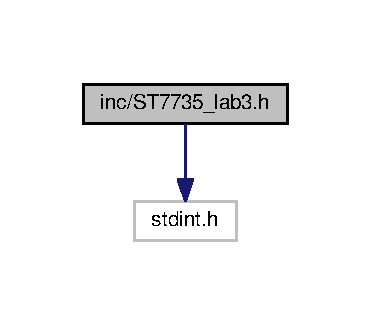
\includegraphics[width=178pt]{ST7735__lab3_8h__incl}
\end{center}
\end{figure}
\subsection*{Macros}
\begin{DoxyCompactItemize}
\item 
\#define {\bfseries S\+T7735\+\_\+\+T\+F\+T\+W\+I\+D\+TH}~128\hypertarget{ST7735__lab3_8h_a17fb18a972efbcba457b22ac53ab39bf}{}\label{ST7735__lab3_8h_a17fb18a972efbcba457b22ac53ab39bf}

\item 
\#define {\bfseries S\+T7735\+\_\+\+T\+F\+T\+H\+E\+I\+G\+HT}~160\hypertarget{ST7735__lab3_8h_ae39c2160287830a930ae303f4d9eb102}{}\label{ST7735__lab3_8h_ae39c2160287830a930ae303f4d9eb102}

\item 
\#define {\bfseries S\+T7735\+\_\+\+B\+L\+A\+CK}~0x0000\hypertarget{ST7735__lab3_8h_aaa96c65299e5f6da446f29dc44362df4}{}\label{ST7735__lab3_8h_aaa96c65299e5f6da446f29dc44362df4}

\item 
\#define {\bfseries S\+T7735\+\_\+\+B\+L\+UE}~0x\+F800\hypertarget{ST7735__lab3_8h_a16ebfdbf93e5ef70d658bf2c38a95939}{}\label{ST7735__lab3_8h_a16ebfdbf93e5ef70d658bf2c38a95939}

\item 
\#define {\bfseries S\+T7735\+\_\+\+R\+ED}~0x001F\hypertarget{ST7735__lab3_8h_a2449a6653137f07d2feb059750c7a0e0}{}\label{ST7735__lab3_8h_a2449a6653137f07d2feb059750c7a0e0}

\item 
\#define {\bfseries S\+T7735\+\_\+\+G\+R\+E\+EN}~0x07\+E0\hypertarget{ST7735__lab3_8h_aaa6015ded61cf7d99ef6d59f1516853a}{}\label{ST7735__lab3_8h_aaa6015ded61cf7d99ef6d59f1516853a}

\item 
\#define {\bfseries S\+T7735\+\_\+\+C\+Y\+AN}~0x\+F\+F\+E0\hypertarget{ST7735__lab3_8h_ad810da70a616c774959a2b8e01bdbccd}{}\label{ST7735__lab3_8h_ad810da70a616c774959a2b8e01bdbccd}

\item 
\#define {\bfseries S\+T7735\+\_\+\+M\+A\+G\+E\+N\+TA}~0x\+F81F\hypertarget{ST7735__lab3_8h_afeb931b9ea5b9e7d1d3034f68da9ca64}{}\label{ST7735__lab3_8h_afeb931b9ea5b9e7d1d3034f68da9ca64}

\item 
\#define {\bfseries S\+T7735\+\_\+\+Y\+E\+L\+L\+OW}~0x07\+FF\hypertarget{ST7735__lab3_8h_ab45f6510169efe9c541a881c8ed56f1c}{}\label{ST7735__lab3_8h_ab45f6510169efe9c541a881c8ed56f1c}

\item 
\#define {\bfseries S\+T7735\+\_\+\+W\+H\+I\+TE}~0x\+F\+F\+FF\hypertarget{ST7735__lab3_8h_af8065f00d6684d4af187dc58b0611af3}{}\label{ST7735__lab3_8h_af8065f00d6684d4af187dc58b0611af3}

\end{DoxyCompactItemize}
\subsection*{Enumerations}
\begin{DoxyCompactItemize}
\item 
enum \hyperlink{ST7735__lab3_8h_a9568e103412377d5867f1f367ac7f424}{init\+R\+Flags} \{ \\*
{\bfseries none}, 
{\bfseries I\+N\+I\+T\+R\+\_\+\+G\+R\+E\+E\+N\+T\+AB}, 
{\bfseries I\+N\+I\+T\+R\+\_\+\+R\+E\+D\+T\+AB}, 
{\bfseries I\+N\+I\+T\+R\+\_\+\+B\+L\+A\+C\+K\+T\+AB}, 
\\*
{\bfseries none}, 
{\bfseries I\+N\+I\+T\+R\+\_\+\+G\+R\+E\+E\+N\+T\+AB}, 
{\bfseries I\+N\+I\+T\+R\+\_\+\+R\+E\+D\+T\+AB}, 
{\bfseries I\+N\+I\+T\+R\+\_\+\+B\+L\+A\+C\+K\+T\+AB}
 \}\hypertarget{ST7735__lab3_8h_a9568e103412377d5867f1f367ac7f424}{}\label{ST7735__lab3_8h_a9568e103412377d5867f1f367ac7f424}
\begin{DoxyCompactList}\small\item\em some flags for \hyperlink{ST7735__lab3_8h_a204a442207d7367ace616bd6bfd79348}{S\+T7735\+\_\+\+Init\+R()} \end{DoxyCompactList}
\end{DoxyCompactItemize}
\subsection*{Functions}
\begin{DoxyCompactItemize}
\item 
void \hyperlink{ST7735__lab3_8h_aec8e637c759ad0adde0758c0935f383a}{S\+T7735\+\_\+\+InitB} (void)\hypertarget{ST7735__lab3_8h_aec8e637c759ad0adde0758c0935f383a}{}\label{ST7735__lab3_8h_aec8e637c759ad0adde0758c0935f383a}

\begin{DoxyCompactList}\small\item\em Initialization for S\+T7735B screens. \end{DoxyCompactList}\item 
void \hyperlink{ST7735__lab3_8h_a204a442207d7367ace616bd6bfd79348}{S\+T7735\+\_\+\+InitR} (enum \hyperlink{ST7735__lab3_8h_a9568e103412377d5867f1f367ac7f424}{init\+R\+Flags} option)
\begin{DoxyCompactList}\small\item\em Initialization for S\+T7735R screens (green or red tabs). \end{DoxyCompactList}\item 
void \hyperlink{ST7735__lab3_8h_aa2dc768f637489753a7b70eac676c4a5}{S\+T7735\+\_\+\+Draw\+Pixel} (int16\+\_\+t x, int16\+\_\+t y, uint16\+\_\+t color)
\begin{DoxyCompactList}\small\item\em Color the pixel at the given coordinates with the given color. Requires 13 bytes of transmission. \end{DoxyCompactList}\item 
void \hyperlink{ST7735__lab3_8h_a2c091bb2f7905e4464a6152015a49989}{S\+T7735\+\_\+\+Draw\+Fast\+V\+Line} (int16\+\_\+t x, int16\+\_\+t y, int16\+\_\+t h, uint16\+\_\+t color)
\begin{DoxyCompactList}\small\item\em Draw a vertical line at the given coordinates with the given height and color. A vertical line is parallel to the longer side of the rectangular display Requires (11 + 2$\ast$h) bytes of transmission (assuming image fully on screen) \end{DoxyCompactList}\item 
void \hyperlink{ST7735__lab3_8h_a05c18aa8dd363fe991d5bc73a02e7abc}{S\+T7735\+\_\+\+Draw\+Fast\+H\+Line} (int16\+\_\+t x, int16\+\_\+t y, int16\+\_\+t w, uint16\+\_\+t color)
\begin{DoxyCompactList}\small\item\em Draw a horizontal line at the given coordinates with the given width and color. A horizontal line is parallel to the shorter side of the rectangular display Requires (11 + 2$\ast$w) bytes of transmission (assuming image fully on screen) \end{DoxyCompactList}\item 
void \hyperlink{ST7735__lab3_8h_a3a14506207ab49aee2c40700b5036271}{S\+T7735\+\_\+\+Fill\+Screen} (uint16\+\_\+t color)
\begin{DoxyCompactList}\small\item\em Fill the screen with the given color. Requires 40,971 bytes of transmission. \end{DoxyCompactList}\item 
void \hyperlink{ST7735__lab3_8h_ada283d88275b972d188afad1c8649829}{S\+T7735\+\_\+\+Fill\+Rect} (int16\+\_\+t x, int16\+\_\+t y, int16\+\_\+t w, int16\+\_\+t h, uint16\+\_\+t color)
\begin{DoxyCompactList}\small\item\em Draw a filled rectangle at the given coordinates with the given width, height, and color. Requires (11 + 2$\ast$w$\ast$h) bytes of transmission (assuming image fully on screen) \end{DoxyCompactList}\item 
uint16\+\_\+t \hyperlink{ST7735__lab3_8h_a29294596f660f05ad8738db73ee07cfa}{S\+T7735\+\_\+\+Color565} (uint8\+\_\+t r, uint8\+\_\+t g, uint8\+\_\+t b)
\begin{DoxyCompactList}\small\item\em Pass 8-\/bit (each) R,G,B and get back 16-\/bit packed color. \end{DoxyCompactList}\item 
uint16\+\_\+t \hyperlink{ST7735__lab3_8h_acd13666f7002b9b8cb7a11164b2203ca}{S\+T7735\+\_\+\+Swap\+Color} (uint16\+\_\+t x)
\begin{DoxyCompactList}\small\item\em Swaps the red and blue values of the given 16-\/bit packed color; green is unchanged. \end{DoxyCompactList}\item 
void \hyperlink{ST7735__lab3_8h_aaf5af072e5213fcc3d6b852a2553e048}{S\+T7735\+\_\+\+Draw\+Bitmap} (int16\+\_\+t x, int16\+\_\+t y, const uint16\+\_\+t $\ast$image, int16\+\_\+t w, int16\+\_\+t h)
\begin{DoxyCompactList}\small\item\em Displays a 16-\/bit color B\+MP image. A bitmap file that is created by a PC image processing program has a header and may be padded with dummy columns so the data have four byte alignment. This function assumes that all of that has been stripped out, and the array image\mbox{[}\mbox{]} has one 16-\/bit halfword for each pixel to be displayed on the screen (encoded in reverse order, which is standard for bitmap files). An array can be created in this format from a 24-\/bit-\/per-\/pixel .bmp file using the associated converter program. (x,y) is the screen location of the lower left corner of B\+MP image Requires (11 + 2$\ast$w$\ast$h) bytes of transmission (assuming image fully on screen) Must be less than or equal to 128 pixels wide by 160 pixels high. \end{DoxyCompactList}\item 
void \hyperlink{ST7735__lab3_8h_a0d092afe5e5a087662adc8e5befa0078}{S\+T7735\+\_\+\+Draw\+CharS} (int16\+\_\+t x, int16\+\_\+t y, char c, int16\+\_\+t text\+Color, int16\+\_\+t bg\+Color, uint8\+\_\+t size)
\begin{DoxyCompactList}\small\item\em Simple character draw function. This is the same function from Adafruit\+\_\+\+G\+F\+X.\+c but adapted for this processor. However, each call to \hyperlink{ST7735__lab3_8h_aa2dc768f637489753a7b70eac676c4a5}{S\+T7735\+\_\+\+Draw\+Pixel()} calls set\+Addr\+Window(), which needs to send many extra data and commands. If the background color is the same as the text color, no background will be printed, and text can be drawn right over existing images without covering them with a box. Requires (11 + 2$\ast$size$\ast$size)$\ast$6$\ast$8 (image fully on screen; textcolor != bg\+Color) \end{DoxyCompactList}\item 
void \hyperlink{ST7735__lab3_8h_a66c54533bdb1555b1e488bb9fcf9885b}{S\+T7735\+\_\+\+Draw\+Char} (int16\+\_\+t x, int16\+\_\+t y, char c, int16\+\_\+t text\+Color, int16\+\_\+t bg\+Color, uint8\+\_\+t size)
\begin{DoxyCompactList}\small\item\em Advanced character draw function. This is similar to the function from Adafruit\+\_\+\+G\+F\+X.\+c but adapted for this processor. However, this function only uses one call to set\+Addr\+Window(), which allows it to run at least twice as fast. Requires (11 + size$\ast$size$\ast$6$\ast$8) bytes of transmission (assuming image fully on screen) \end{DoxyCompactList}\item 
uint32\+\_\+t \hyperlink{ST7735__lab3_8h_a6ba26fa5ccecc77525017d0dcacf037b}{S\+T7735\+\_\+\+Draw\+String} (uint16\+\_\+t x, uint16\+\_\+t y, char $\ast$pt, int16\+\_\+t text\+Color, int16\+\_\+t bg\+Color)
\begin{DoxyCompactList}\small\item\em String draw function. 16 rows (0 to 15) and 21 characters (0 to 20) Requires (11 + size$\ast$size$\ast$6$\ast$8) bytes of transmission for each character If bg\+Color is same as text\+Color, no background will be filled in for chars. \end{DoxyCompactList}\item 
void \hyperlink{ST7735__lab3_8h_a6edc4479f68eb34624157cc1dda2cbb3}{S\+T7735\+\_\+\+Set\+Cursor} (uint32\+\_\+t newX, uint32\+\_\+t newY)
\begin{DoxyCompactList}\small\item\em Move the cursor to the desired X-\/ and Y-\/position. The next character will be printed here. X=0 is the leftmost column. Y=0 is the top row. \end{DoxyCompactList}\item 
void \hyperlink{ST7735__lab3_8h_a072f5f963df6e48f5985977526d2466c}{S\+T7735\+\_\+\+Out\+U\+Dec} (uint32\+\_\+t n)
\begin{DoxyCompactList}\small\item\em Output a 32-\/bit number in unsigned decimal format Position determined by S\+T7735\+\_\+\+Set\+Cursor command Color set by S\+T7735\+\_\+\+Set\+Text\+Color. \end{DoxyCompactList}\item 
void \hyperlink{ST7735__lab3_8h_ac07019a4990ece959dd04dd58339f839}{S\+T7735\+\_\+\+Set\+Rotation} (uint8\+\_\+t m)
\begin{DoxyCompactList}\small\item\em Change the image rotation. Requires 2 bytes of transmission. \end{DoxyCompactList}\item 
void \hyperlink{ST7735__lab3_8h_a2138bd237e97da48ad87137fb616be37}{S\+T7735\+\_\+\+Invert\+Display} (int i)
\begin{DoxyCompactList}\small\item\em Send the command to invert all of the colors. Requires 1 byte of transmission. \end{DoxyCompactList}\item 
void \hyperlink{ST7735__lab3_8h_affbb292ebbf7082c331ab6195da3385c}{S\+T7735\+\_\+\+Plot\+Clear} (int32\+\_\+t ymin, int32\+\_\+t ymax)
\begin{DoxyCompactList}\small\item\em Clear the graphics buffer, set X coordinate to 0 This routine clears the display. \end{DoxyCompactList}\item 
void \hyperlink{ST7735__lab3_8h_a1ae5c293f7cf004c66ca1c0f0d365fcd}{S\+T7735\+\_\+\+Plot\+Point} (int32\+\_\+t y)
\begin{DoxyCompactList}\small\item\em Used in the voltage versus time plot, plot one point at y It does output to display. \end{DoxyCompactList}\item 
void \hyperlink{ST7735__lab3_8h_a3b19f449b1072070e3dd7f92ce8150fa}{S\+T7735\+\_\+\+Plot\+Line} (int32\+\_\+t y)
\begin{DoxyCompactList}\small\item\em Used in the voltage versus time plot, plot line to new point It does output to display. \end{DoxyCompactList}\item 
void \hyperlink{ST7735__lab3_8h_af8a878e2129edc09d38b3f3aadcad42f}{S\+T7735\+\_\+\+Plot\+Points} (int32\+\_\+t y1, int32\+\_\+t y2)
\begin{DoxyCompactList}\small\item\em Used in the voltage versus time plot, plot two points at y1, y2 It does output to display. \end{DoxyCompactList}\item 
void \hyperlink{ST7735__lab3_8h_adff58b909cb89f694117603da4ab7a1b}{S\+T7735\+\_\+\+Plot\+Bar} (int32\+\_\+t y)
\begin{DoxyCompactList}\small\item\em Used in the voltage versus time bar, plot one bar at y It does not output to display until R\+I\+T128x96x4\+Show\+Plot called. \end{DoxyCompactList}\item 
void \hyperlink{ST7735__lab3_8h_a179ccebd4bfe4529903a02ce797e78ea}{S\+T7735\+\_\+\+Plotd\+Bfs} (int32\+\_\+t y)
\begin{DoxyCompactList}\small\item\em Used in the amplitude versus frequency plot, plot bar point at y 0 to 0.\+625V scaled on a log plot from min to max It does output to display. \end{DoxyCompactList}\item 
void \hyperlink{ST7735__lab3_8h_afc91fa494b54f542c2d7cc7ef1fed3e9}{S\+T7735\+\_\+\+Plot\+Next} (void)\hypertarget{ST7735__lab3_8h_afc91fa494b54f542c2d7cc7ef1fed3e9}{}\label{ST7735__lab3_8h_afc91fa494b54f542c2d7cc7ef1fed3e9}

\begin{DoxyCompactList}\small\item\em Used in all the plots to step the X coordinate one pixel X steps from 0 to 127, then back to 0 again It does not output to display. \end{DoxyCompactList}\item 
void \hyperlink{ST7735__lab3_8h_a3c7b330d12b052f9334781dba849aa0e}{S\+T7735\+\_\+\+Plot\+Next\+Erase} (void)\hypertarget{ST7735__lab3_8h_a3c7b330d12b052f9334781dba849aa0e}{}\label{ST7735__lab3_8h_a3c7b330d12b052f9334781dba849aa0e}

\begin{DoxyCompactList}\small\item\em Used in all the plots to step the X coordinate one pixel X steps from 0 to 127, then back to 0 again It clears the vertical space into which the next pixel will be drawn. \end{DoxyCompactList}\item 
void \hyperlink{ST7735__lab3_8h_a49a0a636404c51a7fe1b54768e47d1eb}{S\+T7735\+\_\+\+Out\+Char} (char ch)
\begin{DoxyCompactList}\small\item\em Output one character to the L\+CD Position determined by S\+T7735\+\_\+\+Set\+Cursor command Color set by S\+T7735\+\_\+\+Set\+Text\+Color. \end{DoxyCompactList}\item 
void \hyperlink{ST7735__lab3_8h_a6bd647233ed938c4006694552b8fd9a0}{S\+T7735\+\_\+\+Out\+String} (char $\ast$ptr)
\begin{DoxyCompactList}\small\item\em Print a string of characters to the S\+T7735 L\+CD. Position determined by S\+T7735\+\_\+\+Set\+Cursor command Color set by S\+T7735\+\_\+\+Set\+Text\+Color The string will not automatically wrap. \end{DoxyCompactList}\item 
void \hyperlink{ST7735__lab3_8h_a749b305138c366373f55e39a2ae15f17}{S\+T7735\+\_\+\+Set\+Text\+Color} (uint16\+\_\+t color)
\begin{DoxyCompactList}\small\item\em Sets the color in which the characters will be printed Background color is fixed at black. \end{DoxyCompactList}\item 
void \hyperlink{ST7735__lab3_8h_a8c197f8fb3fd2b2da459e71b44978d53}{Output\+\_\+\+Init} (void)\hypertarget{ST7735__lab3_8h_a8c197f8fb3fd2b2da459e71b44978d53}{}\label{ST7735__lab3_8h_a8c197f8fb3fd2b2da459e71b44978d53}

\begin{DoxyCompactList}\small\item\em Standard device driver initialization function for printf Initialize S\+T7735 L\+CD. \end{DoxyCompactList}\item 
void \hyperlink{ST7735__lab3_8h_a991e9f71a35a1f6ec9d857ca0e01868a}{Output\+\_\+\+Clear} (void)\hypertarget{ST7735__lab3_8h_a991e9f71a35a1f6ec9d857ca0e01868a}{}\label{ST7735__lab3_8h_a991e9f71a35a1f6ec9d857ca0e01868a}

\begin{DoxyCompactList}\small\item\em Clear display. \end{DoxyCompactList}\item 
void \hyperlink{ST7735__lab3_8h_a4ff293d693c5298110cf8a170e9b9165}{Output\+\_\+\+Off} (void)\hypertarget{ST7735__lab3_8h_a4ff293d693c5298110cf8a170e9b9165}{}\label{ST7735__lab3_8h_a4ff293d693c5298110cf8a170e9b9165}

\begin{DoxyCompactList}\small\item\em Turn off display (low power) \end{DoxyCompactList}\item 
void \hyperlink{ST7735__lab3_8h_a7e57930cfb2d70ead5a1686d9f36a734}{Output\+\_\+\+On} (void)\hypertarget{ST7735__lab3_8h_a7e57930cfb2d70ead5a1686d9f36a734}{}\label{ST7735__lab3_8h_a7e57930cfb2d70ead5a1686d9f36a734}

\begin{DoxyCompactList}\small\item\em Turn on display. \end{DoxyCompactList}\item 
void \hyperlink{ST7735__lab3_8h_a1719f525285902712d14efeab76cedcd}{Output\+\_\+\+Color} (uint32\+\_\+t new\+Color)
\begin{DoxyCompactList}\small\item\em set the color for future output Background color is fixed at black \end{DoxyCompactList}\item 
void \hyperlink{ST7735__lab3_8h_a458e4307692b8df8ab1aef53666e1435}{S\+T7735\+\_\+\+Message} (int device, int line, char $\ast$string, int32\+\_\+t value)
\begin{DoxyCompactList}\small\item\em Display a string and number on one of two logical displays at a given line number relative to that display. The L\+CD display is logically divided into two displays\+: top and bottom. These logical displays are identified with a device ID. Device 0 is the top display, device 1 is the bottom display. Each logical device has 4 lines, numbered 0 to 3. Prints in black text on a white background. This function is not (yet) reentrant. \end{DoxyCompactList}\end{DoxyCompactItemize}


\subsection{Detailed Description}
This is a library for the Adafruit 1.\+8" S\+PI display. 



\subsection{Function Documentation}
\index{S\+T7735\+\_\+lab3.\+h@{S\+T7735\+\_\+lab3.\+h}!Output\+\_\+\+Color@{Output\+\_\+\+Color}}
\index{Output\+\_\+\+Color@{Output\+\_\+\+Color}!S\+T7735\+\_\+lab3.\+h@{S\+T7735\+\_\+lab3.\+h}}
\subsubsection[{\texorpdfstring{Output\+\_\+\+Color(uint32\+\_\+t new\+Color)}{Output_Color(uint32_t newColor)}}]{\setlength{\rightskip}{0pt plus 5cm}void Output\+\_\+\+Color (
\begin{DoxyParamCaption}
\item[{uint32\+\_\+t}]{new\+Color}
\end{DoxyParamCaption}
)}\hypertarget{ST7735__lab3_8h_a1719f525285902712d14efeab76cedcd}{}\label{ST7735__lab3_8h_a1719f525285902712d14efeab76cedcd}


set the color for future output Background color is fixed at black 


\begin{DoxyParams}{Parameters}
{\em new\+Color} & 16-\/bit packed color \\
\hline
\end{DoxyParams}
\index{S\+T7735\+\_\+lab3.\+h@{S\+T7735\+\_\+lab3.\+h}!S\+T7735\+\_\+\+Color565@{S\+T7735\+\_\+\+Color565}}
\index{S\+T7735\+\_\+\+Color565@{S\+T7735\+\_\+\+Color565}!S\+T7735\+\_\+lab3.\+h@{S\+T7735\+\_\+lab3.\+h}}
\subsubsection[{\texorpdfstring{S\+T7735\+\_\+\+Color565(uint8\+\_\+t r, uint8\+\_\+t g, uint8\+\_\+t b)}{ST7735_Color565(uint8_t r, uint8_t g, uint8_t b)}}]{\setlength{\rightskip}{0pt plus 5cm}uint16\+\_\+t S\+T7735\+\_\+\+Color565 (
\begin{DoxyParamCaption}
\item[{uint8\+\_\+t}]{r, }
\item[{uint8\+\_\+t}]{g, }
\item[{uint8\+\_\+t}]{b}
\end{DoxyParamCaption}
)}\hypertarget{ST7735__lab3_8h_a29294596f660f05ad8738db73ee07cfa}{}\label{ST7735__lab3_8h_a29294596f660f05ad8738db73ee07cfa}


Pass 8-\/bit (each) R,G,B and get back 16-\/bit packed color. 


\begin{DoxyParams}{Parameters}
{\em r} & red value \\
\hline
{\em g} & green value \\
\hline
{\em b} & blue value \\
\hline
\end{DoxyParams}
\begin{DoxyReturn}{Returns}
uint16\+\_\+t 16-\/bit color 
\end{DoxyReturn}
\index{S\+T7735\+\_\+lab3.\+h@{S\+T7735\+\_\+lab3.\+h}!S\+T7735\+\_\+\+Draw\+Bitmap@{S\+T7735\+\_\+\+Draw\+Bitmap}}
\index{S\+T7735\+\_\+\+Draw\+Bitmap@{S\+T7735\+\_\+\+Draw\+Bitmap}!S\+T7735\+\_\+lab3.\+h@{S\+T7735\+\_\+lab3.\+h}}
\subsubsection[{\texorpdfstring{S\+T7735\+\_\+\+Draw\+Bitmap(int16\+\_\+t x, int16\+\_\+t y, const uint16\+\_\+t $\ast$image, int16\+\_\+t w, int16\+\_\+t h)}{ST7735_DrawBitmap(int16_t x, int16_t y, const uint16_t *image, int16_t w, int16_t h)}}]{\setlength{\rightskip}{0pt plus 5cm}void S\+T7735\+\_\+\+Draw\+Bitmap (
\begin{DoxyParamCaption}
\item[{int16\+\_\+t}]{x, }
\item[{int16\+\_\+t}]{y, }
\item[{const uint16\+\_\+t $\ast$}]{image, }
\item[{int16\+\_\+t}]{w, }
\item[{int16\+\_\+t}]{h}
\end{DoxyParamCaption}
)}\hypertarget{ST7735__lab3_8h_aaf5af072e5213fcc3d6b852a2553e048}{}\label{ST7735__lab3_8h_aaf5af072e5213fcc3d6b852a2553e048}


Displays a 16-\/bit color B\+MP image. A bitmap file that is created by a PC image processing program has a header and may be padded with dummy columns so the data have four byte alignment. This function assumes that all of that has been stripped out, and the array image\mbox{[}\mbox{]} has one 16-\/bit halfword for each pixel to be displayed on the screen (encoded in reverse order, which is standard for bitmap files). An array can be created in this format from a 24-\/bit-\/per-\/pixel .bmp file using the associated converter program. (x,y) is the screen location of the lower left corner of B\+MP image Requires (11 + 2$\ast$w$\ast$h) bytes of transmission (assuming image fully on screen) Must be less than or equal to 128 pixels wide by 160 pixels high. 


\begin{DoxyParams}{Parameters}
{\em x} & horizontal position of the bottom left corner of the image, columns from the left edge \\
\hline
{\em y} & vertical position of the bottom left corner of the image, rows from the top edge \\
\hline
{\em image} & pointer to a 16-\/bit color B\+MP image \\
\hline
{\em w} & number of pixels wide \\
\hline
{\em h} & number of pixels tall \\
\hline
\end{DoxyParams}
\index{S\+T7735\+\_\+lab3.\+h@{S\+T7735\+\_\+lab3.\+h}!S\+T7735\+\_\+\+Draw\+Char@{S\+T7735\+\_\+\+Draw\+Char}}
\index{S\+T7735\+\_\+\+Draw\+Char@{S\+T7735\+\_\+\+Draw\+Char}!S\+T7735\+\_\+lab3.\+h@{S\+T7735\+\_\+lab3.\+h}}
\subsubsection[{\texorpdfstring{S\+T7735\+\_\+\+Draw\+Char(int16\+\_\+t x, int16\+\_\+t y, char c, int16\+\_\+t text\+Color, int16\+\_\+t bg\+Color, uint8\+\_\+t size)}{ST7735_DrawChar(int16_t x, int16_t y, char c, int16_t textColor, int16_t bgColor, uint8_t size)}}]{\setlength{\rightskip}{0pt plus 5cm}void S\+T7735\+\_\+\+Draw\+Char (
\begin{DoxyParamCaption}
\item[{int16\+\_\+t}]{x, }
\item[{int16\+\_\+t}]{y, }
\item[{char}]{c, }
\item[{int16\+\_\+t}]{text\+Color, }
\item[{int16\+\_\+t}]{bg\+Color, }
\item[{uint8\+\_\+t}]{size}
\end{DoxyParamCaption}
)}\hypertarget{ST7735__lab3_8h_a66c54533bdb1555b1e488bb9fcf9885b}{}\label{ST7735__lab3_8h_a66c54533bdb1555b1e488bb9fcf9885b}


Advanced character draw function. This is similar to the function from Adafruit\+\_\+\+G\+F\+X.\+c but adapted for this processor. However, this function only uses one call to set\+Addr\+Window(), which allows it to run at least twice as fast. Requires (11 + size$\ast$size$\ast$6$\ast$8) bytes of transmission (assuming image fully on screen) 


\begin{DoxyParams}{Parameters}
{\em x} & horizontal position of the top left corner of the character, columns from the left edge \\
\hline
{\em y} & vertical position of the top left corner of the character, rows from the top edge \\
\hline
{\em c} & character to be printed \\
\hline
{\em text\+Color} & 16-\/bit color of the character \\
\hline
{\em bg\+Color} & 16-\/bit color of the background \\
\hline
{\em size} & number of pixels per character pixel (e.\+g. size==2 prints each pixel of font as 2x2 square) \\
\hline
\end{DoxyParams}
\index{S\+T7735\+\_\+lab3.\+h@{S\+T7735\+\_\+lab3.\+h}!S\+T7735\+\_\+\+Draw\+CharS@{S\+T7735\+\_\+\+Draw\+CharS}}
\index{S\+T7735\+\_\+\+Draw\+CharS@{S\+T7735\+\_\+\+Draw\+CharS}!S\+T7735\+\_\+lab3.\+h@{S\+T7735\+\_\+lab3.\+h}}
\subsubsection[{\texorpdfstring{S\+T7735\+\_\+\+Draw\+Char\+S(int16\+\_\+t x, int16\+\_\+t y, char c, int16\+\_\+t text\+Color, int16\+\_\+t bg\+Color, uint8\+\_\+t size)}{ST7735_DrawCharS(int16_t x, int16_t y, char c, int16_t textColor, int16_t bgColor, uint8_t size)}}]{\setlength{\rightskip}{0pt plus 5cm}void S\+T7735\+\_\+\+Draw\+CharS (
\begin{DoxyParamCaption}
\item[{int16\+\_\+t}]{x, }
\item[{int16\+\_\+t}]{y, }
\item[{char}]{c, }
\item[{int16\+\_\+t}]{text\+Color, }
\item[{int16\+\_\+t}]{bg\+Color, }
\item[{uint8\+\_\+t}]{size}
\end{DoxyParamCaption}
)}\hypertarget{ST7735__lab3_8h_a0d092afe5e5a087662adc8e5befa0078}{}\label{ST7735__lab3_8h_a0d092afe5e5a087662adc8e5befa0078}


Simple character draw function. This is the same function from Adafruit\+\_\+\+G\+F\+X.\+c but adapted for this processor. However, each call to \hyperlink{ST7735__lab3_8h_aa2dc768f637489753a7b70eac676c4a5}{S\+T7735\+\_\+\+Draw\+Pixel()} calls set\+Addr\+Window(), which needs to send many extra data and commands. If the background color is the same as the text color, no background will be printed, and text can be drawn right over existing images without covering them with a box. Requires (11 + 2$\ast$size$\ast$size)$\ast$6$\ast$8 (image fully on screen; textcolor != bg\+Color) 


\begin{DoxyParams}{Parameters}
{\em x} & horizontal position of the top left corner of the character, columns from the left edge \\
\hline
{\em y} & vertical position of the top left corner of the character, rows from the top edge \\
\hline
{\em c} & character to be printed \\
\hline
{\em text\+Color} & 16-\/bit color of the character \\
\hline
{\em bg\+Color} & 16-\/bit color of the background \\
\hline
{\em size} & number of pixels per character pixel (e.\+g. size==2 prints each pixel of font as 2x2 square) \\
\hline
\end{DoxyParams}
\index{S\+T7735\+\_\+lab3.\+h@{S\+T7735\+\_\+lab3.\+h}!S\+T7735\+\_\+\+Draw\+Fast\+H\+Line@{S\+T7735\+\_\+\+Draw\+Fast\+H\+Line}}
\index{S\+T7735\+\_\+\+Draw\+Fast\+H\+Line@{S\+T7735\+\_\+\+Draw\+Fast\+H\+Line}!S\+T7735\+\_\+lab3.\+h@{S\+T7735\+\_\+lab3.\+h}}
\subsubsection[{\texorpdfstring{S\+T7735\+\_\+\+Draw\+Fast\+H\+Line(int16\+\_\+t x, int16\+\_\+t y, int16\+\_\+t w, uint16\+\_\+t color)}{ST7735_DrawFastHLine(int16_t x, int16_t y, int16_t w, uint16_t color)}}]{\setlength{\rightskip}{0pt plus 5cm}void S\+T7735\+\_\+\+Draw\+Fast\+H\+Line (
\begin{DoxyParamCaption}
\item[{int16\+\_\+t}]{x, }
\item[{int16\+\_\+t}]{y, }
\item[{int16\+\_\+t}]{w, }
\item[{uint16\+\_\+t}]{color}
\end{DoxyParamCaption}
)}\hypertarget{ST7735__lab3_8h_a05c18aa8dd363fe991d5bc73a02e7abc}{}\label{ST7735__lab3_8h_a05c18aa8dd363fe991d5bc73a02e7abc}


Draw a horizontal line at the given coordinates with the given width and color. A horizontal line is parallel to the shorter side of the rectangular display Requires (11 + 2$\ast$w) bytes of transmission (assuming image fully on screen) 


\begin{DoxyParams}{Parameters}
{\em x} & horizontal position of the start of the line, columns from the left edge \\
\hline
{\em y} & vertical position of the start of the line, rows from the top edge \\
\hline
{\em w} & horizontal width of the line \\
\hline
{\em color} & 16-\/bit color, which can be produced by \hyperlink{ST7735__lab3_8h_a29294596f660f05ad8738db73ee07cfa}{S\+T7735\+\_\+\+Color565()} \\
\hline
\end{DoxyParams}
\index{S\+T7735\+\_\+lab3.\+h@{S\+T7735\+\_\+lab3.\+h}!S\+T7735\+\_\+\+Draw\+Fast\+V\+Line@{S\+T7735\+\_\+\+Draw\+Fast\+V\+Line}}
\index{S\+T7735\+\_\+\+Draw\+Fast\+V\+Line@{S\+T7735\+\_\+\+Draw\+Fast\+V\+Line}!S\+T7735\+\_\+lab3.\+h@{S\+T7735\+\_\+lab3.\+h}}
\subsubsection[{\texorpdfstring{S\+T7735\+\_\+\+Draw\+Fast\+V\+Line(int16\+\_\+t x, int16\+\_\+t y, int16\+\_\+t h, uint16\+\_\+t color)}{ST7735_DrawFastVLine(int16_t x, int16_t y, int16_t h, uint16_t color)}}]{\setlength{\rightskip}{0pt plus 5cm}void S\+T7735\+\_\+\+Draw\+Fast\+V\+Line (
\begin{DoxyParamCaption}
\item[{int16\+\_\+t}]{x, }
\item[{int16\+\_\+t}]{y, }
\item[{int16\+\_\+t}]{h, }
\item[{uint16\+\_\+t}]{color}
\end{DoxyParamCaption}
)}\hypertarget{ST7735__lab3_8h_a2c091bb2f7905e4464a6152015a49989}{}\label{ST7735__lab3_8h_a2c091bb2f7905e4464a6152015a49989}


Draw a vertical line at the given coordinates with the given height and color. A vertical line is parallel to the longer side of the rectangular display Requires (11 + 2$\ast$h) bytes of transmission (assuming image fully on screen) 


\begin{DoxyParams}{Parameters}
{\em x} & horizontal position of the start of the line, columns from the left edge \\
\hline
{\em y} & vertical position of the start of the line, rows from the top edge \\
\hline
{\em h} & vertical height of the line \\
\hline
{\em color} & 16-\/bit color, which can be produced by \hyperlink{ST7735__lab3_8h_a29294596f660f05ad8738db73ee07cfa}{S\+T7735\+\_\+\+Color565()} \\
\hline
\end{DoxyParams}
\index{S\+T7735\+\_\+lab3.\+h@{S\+T7735\+\_\+lab3.\+h}!S\+T7735\+\_\+\+Draw\+Pixel@{S\+T7735\+\_\+\+Draw\+Pixel}}
\index{S\+T7735\+\_\+\+Draw\+Pixel@{S\+T7735\+\_\+\+Draw\+Pixel}!S\+T7735\+\_\+lab3.\+h@{S\+T7735\+\_\+lab3.\+h}}
\subsubsection[{\texorpdfstring{S\+T7735\+\_\+\+Draw\+Pixel(int16\+\_\+t x, int16\+\_\+t y, uint16\+\_\+t color)}{ST7735_DrawPixel(int16_t x, int16_t y, uint16_t color)}}]{\setlength{\rightskip}{0pt plus 5cm}void S\+T7735\+\_\+\+Draw\+Pixel (
\begin{DoxyParamCaption}
\item[{int16\+\_\+t}]{x, }
\item[{int16\+\_\+t}]{y, }
\item[{uint16\+\_\+t}]{color}
\end{DoxyParamCaption}
)}\hypertarget{ST7735__lab3_8h_aa2dc768f637489753a7b70eac676c4a5}{}\label{ST7735__lab3_8h_aa2dc768f637489753a7b70eac676c4a5}


Color the pixel at the given coordinates with the given color. Requires 13 bytes of transmission. 


\begin{DoxyParams}{Parameters}
{\em x} & horizontal position of the pixel, columns from the left edge must be less than 128 0 is on the left, 126 is near the right \\
\hline
{\em y} & vertical position of the pixel, rows from the top edge must be less than 160 159 is near the wires, 0 is the side opposite the wires \\
\hline
{\em color} & 16-\/bit color, which can be produced by \hyperlink{ST7735__lab3_8h_a29294596f660f05ad8738db73ee07cfa}{S\+T7735\+\_\+\+Color565()} \\
\hline
\end{DoxyParams}
\index{S\+T7735\+\_\+lab3.\+h@{S\+T7735\+\_\+lab3.\+h}!S\+T7735\+\_\+\+Draw\+String@{S\+T7735\+\_\+\+Draw\+String}}
\index{S\+T7735\+\_\+\+Draw\+String@{S\+T7735\+\_\+\+Draw\+String}!S\+T7735\+\_\+lab3.\+h@{S\+T7735\+\_\+lab3.\+h}}
\subsubsection[{\texorpdfstring{S\+T7735\+\_\+\+Draw\+String(uint16\+\_\+t x, uint16\+\_\+t y, char $\ast$pt, int16\+\_\+t text\+Color, int16\+\_\+t bg\+Color)}{ST7735_DrawString(uint16_t x, uint16_t y, char *pt, int16_t textColor, int16_t bgColor)}}]{\setlength{\rightskip}{0pt plus 5cm}uint32\+\_\+t S\+T7735\+\_\+\+Draw\+String (
\begin{DoxyParamCaption}
\item[{uint16\+\_\+t}]{x, }
\item[{uint16\+\_\+t}]{y, }
\item[{char $\ast$}]{pt, }
\item[{int16\+\_\+t}]{text\+Color, }
\item[{int16\+\_\+t}]{bg\+Color}
\end{DoxyParamCaption}
)}\hypertarget{ST7735__lab3_8h_a6ba26fa5ccecc77525017d0dcacf037b}{}\label{ST7735__lab3_8h_a6ba26fa5ccecc77525017d0dcacf037b}


String draw function. 16 rows (0 to 15) and 21 characters (0 to 20) Requires (11 + size$\ast$size$\ast$6$\ast$8) bytes of transmission for each character If bg\+Color is same as text\+Color, no background will be filled in for chars. 


\begin{DoxyParams}{Parameters}
{\em x} & columns from the left edge (0 to 20) \\
\hline
{\em y} & rows from the top edge (0 to 15) \\
\hline
{\em pt} & pointer to a null terminated string to be printed \\
\hline
{\em text\+Color} & 16-\/bit color of the characters \\
\hline
{\em bg\+Color} & 16-\/bit color of the background \\
\hline
\end{DoxyParams}
\begin{DoxyReturn}{Returns}
uint32\+\_\+t number of characters printed 
\end{DoxyReturn}
\index{S\+T7735\+\_\+lab3.\+h@{S\+T7735\+\_\+lab3.\+h}!S\+T7735\+\_\+\+Fill\+Rect@{S\+T7735\+\_\+\+Fill\+Rect}}
\index{S\+T7735\+\_\+\+Fill\+Rect@{S\+T7735\+\_\+\+Fill\+Rect}!S\+T7735\+\_\+lab3.\+h@{S\+T7735\+\_\+lab3.\+h}}
\subsubsection[{\texorpdfstring{S\+T7735\+\_\+\+Fill\+Rect(int16\+\_\+t x, int16\+\_\+t y, int16\+\_\+t w, int16\+\_\+t h, uint16\+\_\+t color)}{ST7735_FillRect(int16_t x, int16_t y, int16_t w, int16_t h, uint16_t color)}}]{\setlength{\rightskip}{0pt plus 5cm}void S\+T7735\+\_\+\+Fill\+Rect (
\begin{DoxyParamCaption}
\item[{int16\+\_\+t}]{x, }
\item[{int16\+\_\+t}]{y, }
\item[{int16\+\_\+t}]{w, }
\item[{int16\+\_\+t}]{h, }
\item[{uint16\+\_\+t}]{color}
\end{DoxyParamCaption}
)}\hypertarget{ST7735__lab3_8h_ada283d88275b972d188afad1c8649829}{}\label{ST7735__lab3_8h_ada283d88275b972d188afad1c8649829}


Draw a filled rectangle at the given coordinates with the given width, height, and color. Requires (11 + 2$\ast$w$\ast$h) bytes of transmission (assuming image fully on screen) 


\begin{DoxyParams}{Parameters}
{\em x} & horizontal position of the top left corner of the rectangle, columns from the left edge \\
\hline
{\em y} & vertical position of the top left corner of the rectangle, rows from the top edge \\
\hline
{\em w} & horizontal width of the rectangle \\
\hline
{\em h} & vertical height of the rectangle \\
\hline
{\em color} & 16-\/bit color, which can be produced by \hyperlink{ST7735__lab3_8h_a29294596f660f05ad8738db73ee07cfa}{S\+T7735\+\_\+\+Color565()} \\
\hline
\end{DoxyParams}
\index{S\+T7735\+\_\+lab3.\+h@{S\+T7735\+\_\+lab3.\+h}!S\+T7735\+\_\+\+Fill\+Screen@{S\+T7735\+\_\+\+Fill\+Screen}}
\index{S\+T7735\+\_\+\+Fill\+Screen@{S\+T7735\+\_\+\+Fill\+Screen}!S\+T7735\+\_\+lab3.\+h@{S\+T7735\+\_\+lab3.\+h}}
\subsubsection[{\texorpdfstring{S\+T7735\+\_\+\+Fill\+Screen(uint16\+\_\+t color)}{ST7735_FillScreen(uint16_t color)}}]{\setlength{\rightskip}{0pt plus 5cm}void S\+T7735\+\_\+\+Fill\+Screen (
\begin{DoxyParamCaption}
\item[{uint16\+\_\+t}]{color}
\end{DoxyParamCaption}
)}\hypertarget{ST7735__lab3_8h_a3a14506207ab49aee2c40700b5036271}{}\label{ST7735__lab3_8h_a3a14506207ab49aee2c40700b5036271}


Fill the screen with the given color. Requires 40,971 bytes of transmission. 


\begin{DoxyParams}{Parameters}
{\em color} & 16-\/bit color, which can be produced by \hyperlink{ST7735__lab3_8h_a29294596f660f05ad8738db73ee07cfa}{S\+T7735\+\_\+\+Color565()} \\
\hline
\end{DoxyParams}
\index{S\+T7735\+\_\+lab3.\+h@{S\+T7735\+\_\+lab3.\+h}!S\+T7735\+\_\+\+InitR@{S\+T7735\+\_\+\+InitR}}
\index{S\+T7735\+\_\+\+InitR@{S\+T7735\+\_\+\+InitR}!S\+T7735\+\_\+lab3.\+h@{S\+T7735\+\_\+lab3.\+h}}
\subsubsection[{\texorpdfstring{S\+T7735\+\_\+\+Init\+R(enum init\+R\+Flags option)}{ST7735_InitR(enum initRFlags option)}}]{\setlength{\rightskip}{0pt plus 5cm}void S\+T7735\+\_\+\+InitR (
\begin{DoxyParamCaption}
\item[{enum {\bf init\+R\+Flags}}]{option}
\end{DoxyParamCaption}
)}\hypertarget{ST7735__lab3_8h_a204a442207d7367ace616bd6bfd79348}{}\label{ST7735__lab3_8h_a204a442207d7367ace616bd6bfd79348}


Initialization for S\+T7735R screens (green or red tabs). 


\begin{DoxyParams}{Parameters}
{\em init\+R\+Flags} & one of the enumerated options depending on tabs \\
\hline
\end{DoxyParams}
\index{S\+T7735\+\_\+lab3.\+h@{S\+T7735\+\_\+lab3.\+h}!S\+T7735\+\_\+\+Invert\+Display@{S\+T7735\+\_\+\+Invert\+Display}}
\index{S\+T7735\+\_\+\+Invert\+Display@{S\+T7735\+\_\+\+Invert\+Display}!S\+T7735\+\_\+lab3.\+h@{S\+T7735\+\_\+lab3.\+h}}
\subsubsection[{\texorpdfstring{S\+T7735\+\_\+\+Invert\+Display(int i)}{ST7735_InvertDisplay(int i)}}]{\setlength{\rightskip}{0pt plus 5cm}void S\+T7735\+\_\+\+Invert\+Display (
\begin{DoxyParamCaption}
\item[{int}]{i}
\end{DoxyParamCaption}
)}\hypertarget{ST7735__lab3_8h_a2138bd237e97da48ad87137fb616be37}{}\label{ST7735__lab3_8h_a2138bd237e97da48ad87137fb616be37}


Send the command to invert all of the colors. Requires 1 byte of transmission. 


\begin{DoxyParams}{Parameters}
{\em i} & 0 to disable inversion; non-\/zero to enable inversion \\
\hline
\end{DoxyParams}
\index{S\+T7735\+\_\+lab3.\+h@{S\+T7735\+\_\+lab3.\+h}!S\+T7735\+\_\+\+Message@{S\+T7735\+\_\+\+Message}}
\index{S\+T7735\+\_\+\+Message@{S\+T7735\+\_\+\+Message}!S\+T7735\+\_\+lab3.\+h@{S\+T7735\+\_\+lab3.\+h}}
\subsubsection[{\texorpdfstring{S\+T7735\+\_\+\+Message(int device, int line, char $\ast$string, int32\+\_\+t value)}{ST7735_Message(int device, int line, char *string, int32_t value)}}]{\setlength{\rightskip}{0pt plus 5cm}void S\+T7735\+\_\+\+Message (
\begin{DoxyParamCaption}
\item[{int}]{device, }
\item[{int}]{line, }
\item[{char $\ast$}]{string, }
\item[{int32\+\_\+t}]{value}
\end{DoxyParamCaption}
)}\hypertarget{ST7735__lab3_8h_a458e4307692b8df8ab1aef53666e1435}{}\label{ST7735__lab3_8h_a458e4307692b8df8ab1aef53666e1435}


Display a string and number on one of two logical displays at a given line number relative to that display. The L\+CD display is logically divided into two displays\+: top and bottom. These logical displays are identified with a device ID. Device 0 is the top display, device 1 is the bottom display. Each logical device has 4 lines, numbered 0 to 3. Prints in black text on a white background. This function is not (yet) reentrant. 


\begin{DoxyParams}{Parameters}
{\em device} & Device ID, 0 or 1 \\
\hline
{\em line} & Line number, 0 to 3, relative to the logical display. \\
\hline
{\em string} & Null-\/terminated string to print on the select logical display and line. \\
\hline
{\em value} & Integer value printed after the string. \\
\hline
\end{DoxyParams}
\index{S\+T7735\+\_\+lab3.\+h@{S\+T7735\+\_\+lab3.\+h}!S\+T7735\+\_\+\+Out\+Char@{S\+T7735\+\_\+\+Out\+Char}}
\index{S\+T7735\+\_\+\+Out\+Char@{S\+T7735\+\_\+\+Out\+Char}!S\+T7735\+\_\+lab3.\+h@{S\+T7735\+\_\+lab3.\+h}}
\subsubsection[{\texorpdfstring{S\+T7735\+\_\+\+Out\+Char(char ch)}{ST7735_OutChar(char ch)}}]{\setlength{\rightskip}{0pt plus 5cm}void S\+T7735\+\_\+\+Out\+Char (
\begin{DoxyParamCaption}
\item[{char}]{ch}
\end{DoxyParamCaption}
)}\hypertarget{ST7735__lab3_8h_a49a0a636404c51a7fe1b54768e47d1eb}{}\label{ST7735__lab3_8h_a49a0a636404c51a7fe1b54768e47d1eb}


Output one character to the L\+CD Position determined by S\+T7735\+\_\+\+Set\+Cursor command Color set by S\+T7735\+\_\+\+Set\+Text\+Color. 


\begin{DoxyParams}{Parameters}
{\em ch} & 8-\/bit A\+S\+C\+II character \\
\hline
\end{DoxyParams}
\index{S\+T7735\+\_\+lab3.\+h@{S\+T7735\+\_\+lab3.\+h}!S\+T7735\+\_\+\+Out\+String@{S\+T7735\+\_\+\+Out\+String}}
\index{S\+T7735\+\_\+\+Out\+String@{S\+T7735\+\_\+\+Out\+String}!S\+T7735\+\_\+lab3.\+h@{S\+T7735\+\_\+lab3.\+h}}
\subsubsection[{\texorpdfstring{S\+T7735\+\_\+\+Out\+String(char $\ast$ptr)}{ST7735_OutString(char *ptr)}}]{\setlength{\rightskip}{0pt plus 5cm}void S\+T7735\+\_\+\+Out\+String (
\begin{DoxyParamCaption}
\item[{char $\ast$}]{ptr}
\end{DoxyParamCaption}
)}\hypertarget{ST7735__lab3_8h_a6bd647233ed938c4006694552b8fd9a0}{}\label{ST7735__lab3_8h_a6bd647233ed938c4006694552b8fd9a0}


Print a string of characters to the S\+T7735 L\+CD. Position determined by S\+T7735\+\_\+\+Set\+Cursor command Color set by S\+T7735\+\_\+\+Set\+Text\+Color The string will not automatically wrap. 


\begin{DoxyParams}{Parameters}
{\em ptr} & pointer to N\+U\+L\+L-\/terminated A\+S\+C\+II string \\
\hline
\end{DoxyParams}
\index{S\+T7735\+\_\+lab3.\+h@{S\+T7735\+\_\+lab3.\+h}!S\+T7735\+\_\+\+Out\+U\+Dec@{S\+T7735\+\_\+\+Out\+U\+Dec}}
\index{S\+T7735\+\_\+\+Out\+U\+Dec@{S\+T7735\+\_\+\+Out\+U\+Dec}!S\+T7735\+\_\+lab3.\+h@{S\+T7735\+\_\+lab3.\+h}}
\subsubsection[{\texorpdfstring{S\+T7735\+\_\+\+Out\+U\+Dec(uint32\+\_\+t n)}{ST7735_OutUDec(uint32_t n)}}]{\setlength{\rightskip}{0pt plus 5cm}void S\+T7735\+\_\+\+Out\+U\+Dec (
\begin{DoxyParamCaption}
\item[{uint32\+\_\+t}]{n}
\end{DoxyParamCaption}
)}\hypertarget{ST7735__lab3_8h_a072f5f963df6e48f5985977526d2466c}{}\label{ST7735__lab3_8h_a072f5f963df6e48f5985977526d2466c}


Output a 32-\/bit number in unsigned decimal format Position determined by S\+T7735\+\_\+\+Set\+Cursor command Color set by S\+T7735\+\_\+\+Set\+Text\+Color. 


\begin{DoxyParams}{Parameters}
{\em n} & 32-\/bit number to be transferred \\
\hline
\end{DoxyParams}
\index{S\+T7735\+\_\+lab3.\+h@{S\+T7735\+\_\+lab3.\+h}!S\+T7735\+\_\+\+Plot\+Bar@{S\+T7735\+\_\+\+Plot\+Bar}}
\index{S\+T7735\+\_\+\+Plot\+Bar@{S\+T7735\+\_\+\+Plot\+Bar}!S\+T7735\+\_\+lab3.\+h@{S\+T7735\+\_\+lab3.\+h}}
\subsubsection[{\texorpdfstring{S\+T7735\+\_\+\+Plot\+Bar(int32\+\_\+t y)}{ST7735_PlotBar(int32_t y)}}]{\setlength{\rightskip}{0pt plus 5cm}void S\+T7735\+\_\+\+Plot\+Bar (
\begin{DoxyParamCaption}
\item[{int32\+\_\+t}]{y}
\end{DoxyParamCaption}
)}\hypertarget{ST7735__lab3_8h_adff58b909cb89f694117603da4ab7a1b}{}\label{ST7735__lab3_8h_adff58b909cb89f694117603da4ab7a1b}


Used in the voltage versus time bar, plot one bar at y It does not output to display until R\+I\+T128x96x4\+Show\+Plot called. 


\begin{DoxyParams}{Parameters}
{\em y} & the y coordinate of the bar plotted \\
\hline
\end{DoxyParams}
\index{S\+T7735\+\_\+lab3.\+h@{S\+T7735\+\_\+lab3.\+h}!S\+T7735\+\_\+\+Plot\+Clear@{S\+T7735\+\_\+\+Plot\+Clear}}
\index{S\+T7735\+\_\+\+Plot\+Clear@{S\+T7735\+\_\+\+Plot\+Clear}!S\+T7735\+\_\+lab3.\+h@{S\+T7735\+\_\+lab3.\+h}}
\subsubsection[{\texorpdfstring{S\+T7735\+\_\+\+Plot\+Clear(int32\+\_\+t ymin, int32\+\_\+t ymax)}{ST7735_PlotClear(int32_t ymin, int32_t ymax)}}]{\setlength{\rightskip}{0pt plus 5cm}void S\+T7735\+\_\+\+Plot\+Clear (
\begin{DoxyParamCaption}
\item[{int32\+\_\+t}]{ymin, }
\item[{int32\+\_\+t}]{ymax}
\end{DoxyParamCaption}
)}\hypertarget{ST7735__lab3_8h_affbb292ebbf7082c331ab6195da3385c}{}\label{ST7735__lab3_8h_affbb292ebbf7082c331ab6195da3385c}


Clear the graphics buffer, set X coordinate to 0 This routine clears the display. 


\begin{DoxyParams}{Parameters}
{\em ymin} & Lower bound of plot \\
\hline
{\em ymax} & Upper bound of plot \\
\hline
\end{DoxyParams}
\index{S\+T7735\+\_\+lab3.\+h@{S\+T7735\+\_\+lab3.\+h}!S\+T7735\+\_\+\+Plotd\+Bfs@{S\+T7735\+\_\+\+Plotd\+Bfs}}
\index{S\+T7735\+\_\+\+Plotd\+Bfs@{S\+T7735\+\_\+\+Plotd\+Bfs}!S\+T7735\+\_\+lab3.\+h@{S\+T7735\+\_\+lab3.\+h}}
\subsubsection[{\texorpdfstring{S\+T7735\+\_\+\+Plotd\+Bfs(int32\+\_\+t y)}{ST7735_PlotdBfs(int32_t y)}}]{\setlength{\rightskip}{0pt plus 5cm}void S\+T7735\+\_\+\+Plotd\+Bfs (
\begin{DoxyParamCaption}
\item[{int32\+\_\+t}]{y}
\end{DoxyParamCaption}
)}\hypertarget{ST7735__lab3_8h_a179ccebd4bfe4529903a02ce797e78ea}{}\label{ST7735__lab3_8h_a179ccebd4bfe4529903a02ce797e78ea}


Used in the amplitude versus frequency plot, plot bar point at y 0 to 0.\+625V scaled on a log plot from min to max It does output to display. 


\begin{DoxyParams}{Parameters}
{\em y} & the y A\+DC value of the bar plotted \\
\hline
\end{DoxyParams}
\index{S\+T7735\+\_\+lab3.\+h@{S\+T7735\+\_\+lab3.\+h}!S\+T7735\+\_\+\+Plot\+Line@{S\+T7735\+\_\+\+Plot\+Line}}
\index{S\+T7735\+\_\+\+Plot\+Line@{S\+T7735\+\_\+\+Plot\+Line}!S\+T7735\+\_\+lab3.\+h@{S\+T7735\+\_\+lab3.\+h}}
\subsubsection[{\texorpdfstring{S\+T7735\+\_\+\+Plot\+Line(int32\+\_\+t y)}{ST7735_PlotLine(int32_t y)}}]{\setlength{\rightskip}{0pt plus 5cm}void S\+T7735\+\_\+\+Plot\+Line (
\begin{DoxyParamCaption}
\item[{int32\+\_\+t}]{y}
\end{DoxyParamCaption}
)}\hypertarget{ST7735__lab3_8h_a3b19f449b1072070e3dd7f92ce8150fa}{}\label{ST7735__lab3_8h_a3b19f449b1072070e3dd7f92ce8150fa}


Used in the voltage versus time plot, plot line to new point It does output to display. 


\begin{DoxyParams}{Parameters}
{\em y} & the y coordinate of the point plotted \\
\hline
\end{DoxyParams}
\index{S\+T7735\+\_\+lab3.\+h@{S\+T7735\+\_\+lab3.\+h}!S\+T7735\+\_\+\+Plot\+Point@{S\+T7735\+\_\+\+Plot\+Point}}
\index{S\+T7735\+\_\+\+Plot\+Point@{S\+T7735\+\_\+\+Plot\+Point}!S\+T7735\+\_\+lab3.\+h@{S\+T7735\+\_\+lab3.\+h}}
\subsubsection[{\texorpdfstring{S\+T7735\+\_\+\+Plot\+Point(int32\+\_\+t y)}{ST7735_PlotPoint(int32_t y)}}]{\setlength{\rightskip}{0pt plus 5cm}void S\+T7735\+\_\+\+Plot\+Point (
\begin{DoxyParamCaption}
\item[{int32\+\_\+t}]{y}
\end{DoxyParamCaption}
)}\hypertarget{ST7735__lab3_8h_a1ae5c293f7cf004c66ca1c0f0d365fcd}{}\label{ST7735__lab3_8h_a1ae5c293f7cf004c66ca1c0f0d365fcd}


Used in the voltage versus time plot, plot one point at y It does output to display. 


\begin{DoxyParams}{Parameters}
{\em y} & the y coordinate of the point plotted \\
\hline
\end{DoxyParams}
\index{S\+T7735\+\_\+lab3.\+h@{S\+T7735\+\_\+lab3.\+h}!S\+T7735\+\_\+\+Plot\+Points@{S\+T7735\+\_\+\+Plot\+Points}}
\index{S\+T7735\+\_\+\+Plot\+Points@{S\+T7735\+\_\+\+Plot\+Points}!S\+T7735\+\_\+lab3.\+h@{S\+T7735\+\_\+lab3.\+h}}
\subsubsection[{\texorpdfstring{S\+T7735\+\_\+\+Plot\+Points(int32\+\_\+t y1, int32\+\_\+t y2)}{ST7735_PlotPoints(int32_t y1, int32_t y2)}}]{\setlength{\rightskip}{0pt plus 5cm}void S\+T7735\+\_\+\+Plot\+Points (
\begin{DoxyParamCaption}
\item[{int32\+\_\+t}]{y1, }
\item[{int32\+\_\+t}]{y2}
\end{DoxyParamCaption}
)}\hypertarget{ST7735__lab3_8h_af8a878e2129edc09d38b3f3aadcad42f}{}\label{ST7735__lab3_8h_af8a878e2129edc09d38b3f3aadcad42f}


Used in the voltage versus time plot, plot two points at y1, y2 It does output to display. 


\begin{DoxyParams}{Parameters}
{\em y1} & the y coordinate of the first point plotted \\
\hline
{\em y2} & the y coordinate of the second point plotted \\
\hline
\end{DoxyParams}
\index{S\+T7735\+\_\+lab3.\+h@{S\+T7735\+\_\+lab3.\+h}!S\+T7735\+\_\+\+Set\+Cursor@{S\+T7735\+\_\+\+Set\+Cursor}}
\index{S\+T7735\+\_\+\+Set\+Cursor@{S\+T7735\+\_\+\+Set\+Cursor}!S\+T7735\+\_\+lab3.\+h@{S\+T7735\+\_\+lab3.\+h}}
\subsubsection[{\texorpdfstring{S\+T7735\+\_\+\+Set\+Cursor(uint32\+\_\+t new\+X, uint32\+\_\+t new\+Y)}{ST7735_SetCursor(uint32_t newX, uint32_t newY)}}]{\setlength{\rightskip}{0pt plus 5cm}void S\+T7735\+\_\+\+Set\+Cursor (
\begin{DoxyParamCaption}
\item[{uint32\+\_\+t}]{newX, }
\item[{uint32\+\_\+t}]{newY}
\end{DoxyParamCaption}
)}\hypertarget{ST7735__lab3_8h_a6edc4479f68eb34624157cc1dda2cbb3}{}\label{ST7735__lab3_8h_a6edc4479f68eb34624157cc1dda2cbb3}


Move the cursor to the desired X-\/ and Y-\/position. The next character will be printed here. X=0 is the leftmost column. Y=0 is the top row. 


\begin{DoxyParams}{Parameters}
{\em newX} & new X-\/position of the cursor (0$<$=newX$<$=20) \\
\hline
{\em newY} & new Y-\/position of the cursor (0$<$=newY$<$=15) \\
\hline
\end{DoxyParams}
\index{S\+T7735\+\_\+lab3.\+h@{S\+T7735\+\_\+lab3.\+h}!S\+T7735\+\_\+\+Set\+Rotation@{S\+T7735\+\_\+\+Set\+Rotation}}
\index{S\+T7735\+\_\+\+Set\+Rotation@{S\+T7735\+\_\+\+Set\+Rotation}!S\+T7735\+\_\+lab3.\+h@{S\+T7735\+\_\+lab3.\+h}}
\subsubsection[{\texorpdfstring{S\+T7735\+\_\+\+Set\+Rotation(uint8\+\_\+t m)}{ST7735_SetRotation(uint8_t m)}}]{\setlength{\rightskip}{0pt plus 5cm}void S\+T7735\+\_\+\+Set\+Rotation (
\begin{DoxyParamCaption}
\item[{uint8\+\_\+t}]{m}
\end{DoxyParamCaption}
)}\hypertarget{ST7735__lab3_8h_ac07019a4990ece959dd04dd58339f839}{}\label{ST7735__lab3_8h_ac07019a4990ece959dd04dd58339f839}


Change the image rotation. Requires 2 bytes of transmission. 


\begin{DoxyParams}{Parameters}
{\em m} & new rotation value (0 to 3) \\
\hline
\end{DoxyParams}
\index{S\+T7735\+\_\+lab3.\+h@{S\+T7735\+\_\+lab3.\+h}!S\+T7735\+\_\+\+Set\+Text\+Color@{S\+T7735\+\_\+\+Set\+Text\+Color}}
\index{S\+T7735\+\_\+\+Set\+Text\+Color@{S\+T7735\+\_\+\+Set\+Text\+Color}!S\+T7735\+\_\+lab3.\+h@{S\+T7735\+\_\+lab3.\+h}}
\subsubsection[{\texorpdfstring{S\+T7735\+\_\+\+Set\+Text\+Color(uint16\+\_\+t color)}{ST7735_SetTextColor(uint16_t color)}}]{\setlength{\rightskip}{0pt plus 5cm}void S\+T7735\+\_\+\+Set\+Text\+Color (
\begin{DoxyParamCaption}
\item[{uint16\+\_\+t}]{color}
\end{DoxyParamCaption}
)}\hypertarget{ST7735__lab3_8h_a749b305138c366373f55e39a2ae15f17}{}\label{ST7735__lab3_8h_a749b305138c366373f55e39a2ae15f17}


Sets the color in which the characters will be printed Background color is fixed at black. 


\begin{DoxyParams}{Parameters}
{\em color} & 16-\/bit packed color \\
\hline
\end{DoxyParams}
\index{S\+T7735\+\_\+lab3.\+h@{S\+T7735\+\_\+lab3.\+h}!S\+T7735\+\_\+\+Swap\+Color@{S\+T7735\+\_\+\+Swap\+Color}}
\index{S\+T7735\+\_\+\+Swap\+Color@{S\+T7735\+\_\+\+Swap\+Color}!S\+T7735\+\_\+lab3.\+h@{S\+T7735\+\_\+lab3.\+h}}
\subsubsection[{\texorpdfstring{S\+T7735\+\_\+\+Swap\+Color(uint16\+\_\+t x)}{ST7735_SwapColor(uint16_t x)}}]{\setlength{\rightskip}{0pt plus 5cm}uint16\+\_\+t S\+T7735\+\_\+\+Swap\+Color (
\begin{DoxyParamCaption}
\item[{uint16\+\_\+t}]{x}
\end{DoxyParamCaption}
)}\hypertarget{ST7735__lab3_8h_acd13666f7002b9b8cb7a11164b2203ca}{}\label{ST7735__lab3_8h_acd13666f7002b9b8cb7a11164b2203ca}


Swaps the red and blue values of the given 16-\/bit packed color; green is unchanged. 


\begin{DoxyParams}{Parameters}
{\em x} & 16-\/bit color in format B, G, R \\
\hline
\end{DoxyParams}
\begin{DoxyReturn}{Returns}
uint16\+\_\+t 16-\/bit color in format R, G, B 
\end{DoxyReturn}

\hypertarget{UART_8h}{}\section{inc/\+U\+A\+RT.h File Reference}
\label{UART_8h}\index{inc/\+U\+A\+R\+T.\+h@{inc/\+U\+A\+R\+T.\+h}}


Runs on L\+M4\+F120/\+T\+M4\+C123 Use U\+A\+R\+T0 to implement bidirectional data transfer to and from a computer running Hyper\+Terminal. This time, interrupts and F\+I\+F\+Os are used.  


{\ttfamily \#include $<$stdint.\+h$>$}\\*
Include dependency graph for U\+A\+R\+T.\+h\+:
\nopagebreak
\begin{figure}[H]
\begin{center}
\leavevmode
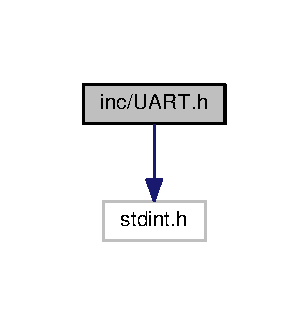
\includegraphics[width=148pt]{UART_8h__incl}
\end{center}
\end{figure}
\subsection*{Macros}
\begin{DoxyCompactItemize}
\item 
\#define {\bfseries CR}~0x0D\hypertarget{UART_8h_a876ce77f3c672c7162658151e648389e}{}\label{UART_8h_a876ce77f3c672c7162658151e648389e}

\item 
\#define {\bfseries LF}~0x0A\hypertarget{UART_8h_a350c9d6cb81908d59427ee96844d1a9c}{}\label{UART_8h_a350c9d6cb81908d59427ee96844d1a9c}

\item 
\#define {\bfseries BS}~0x08\hypertarget{UART_8h_a580a88f98668df1ac5e1683cae31c0b3}{}\label{UART_8h_a580a88f98668df1ac5e1683cae31c0b3}

\item 
\#define {\bfseries E\+SC}~0x1B\hypertarget{UART_8h_a4af1b6159e447ba72652bb7fcdfa726e}{}\label{UART_8h_a4af1b6159e447ba72652bb7fcdfa726e}

\item 
\#define {\bfseries SP}~0x20\hypertarget{UART_8h_aecd69d9a67487cc45c38eb184c50538a}{}\label{UART_8h_aecd69d9a67487cc45c38eb184c50538a}

\item 
\#define {\bfseries D\+EL}~0x7F\hypertarget{UART_8h_ad1e508e805e4ddbc05119be4bb260985}{}\label{UART_8h_ad1e508e805e4ddbc05119be4bb260985}

\end{DoxyCompactItemize}
\subsection*{Functions}
\begin{DoxyCompactItemize}
\item 
void \hyperlink{UART_8h_ad5cbed2a2222bb84e8b5c1caaa50634e}{U\+A\+R\+T\+\_\+\+Init} (void)\hypertarget{UART_8h_ad5cbed2a2222bb84e8b5c1caaa50634e}{}\label{UART_8h_ad5cbed2a2222bb84e8b5c1caaa50634e}

\begin{DoxyCompactList}\small\item\em Initialize the U\+A\+RT for 115,200 baud rate (assuming 50 M\+Hz clock), 8 bit word length, no parity bits, one stop bit, F\+I\+F\+Os enabled. \end{DoxyCompactList}\item 
char \hyperlink{UART_8h_a00e894bb188320a2f4dcd5a78b80da52}{U\+A\+R\+T\+\_\+\+In\+Char} (void)
\begin{DoxyCompactList}\small\item\em Wait for new serial port input. \end{DoxyCompactList}\item 
void \hyperlink{UART_8h_a4ef2f92682b12a347cf1f81cccda4da7}{U\+A\+R\+T\+\_\+\+Out\+Char} (char data)
\begin{DoxyCompactList}\small\item\em 8-\/bit to serial port \end{DoxyCompactList}\item 
void \hyperlink{UART_8h_a2cbbed822dc8e6d801e6c9f21a2cd418}{U\+A\+R\+T\+\_\+\+Out\+String} (char $\ast$pt)
\begin{DoxyCompactList}\small\item\em Output String (N\+U\+LL termination) \end{DoxyCompactList}\item 
uint32\+\_\+t \hyperlink{UART_8h_a0a28a219c31df1bd2182e4b3afbcc5cd}{U\+A\+R\+T\+\_\+\+In\+U\+Dec} (void)
\begin{DoxyCompactList}\small\item\em In\+U\+Dec accepts A\+S\+C\+II input in unsigned decimal format and converts to a 32-\/bit unsigned number valid range is 0 to 4294967295 (2$^\wedge$32-\/1) If you enter a number above 4294967295, it will return an incorrect value Backspace will remove last digit typed. \end{DoxyCompactList}\item 
void \hyperlink{UART_8h_a9a53c5fe8486e0282990b11a218c2625}{U\+A\+R\+T\+\_\+\+Out\+U\+Dec} (uint32\+\_\+t n)
\begin{DoxyCompactList}\small\item\em Output a 32-\/bit number in unsigned decimal format. \end{DoxyCompactList}\item 
uint32\+\_\+t \hyperlink{UART_8h_a5a7efc717f2c844f08689418dd50ee43}{U\+A\+R\+T\+\_\+\+In\+U\+Hex} (void)
\begin{DoxyCompactList}\small\item\em Accepts A\+S\+C\+II input in unsigned hexadecimal (base 16) format No \textquotesingle{}\$\textquotesingle{} or \textquotesingle{}0x\textquotesingle{} need be entered, just the 1 to 8 hex digits It will convert lower case a-\/f to uppercase A-\/F and converts to a 16 bit unsigned number value range is 0 to F\+F\+F\+F\+F\+F\+FF If you enter a number above F\+F\+F\+F\+F\+F\+FF, it will return an incorrect value Backspace will remove last digit typed. \end{DoxyCompactList}\item 
void \hyperlink{UART_8h_a21661aabfda94ec88e9514856f062a41}{U\+A\+R\+T\+\_\+\+Out\+U\+Hex} (uint32\+\_\+t number)
\begin{DoxyCompactList}\small\item\em Output a 32-\/bit number in unsigned hexadecimal format Variable format 1 to 8 digits with no space before or after. \end{DoxyCompactList}\item 
void \hyperlink{UART_8h_a4278ab3463fadff60a5a84792707c3a3}{U\+A\+R\+T\+\_\+\+In\+String} (char $\ast$buf\+Pt, uint16\+\_\+t max)
\begin{DoxyCompactList}\small\item\em Accepts A\+S\+C\+II characters from the serial port and adds them to a string until $<$enter$>$ is typed or until max length of the string is reached. It echoes each character as it is inputted. If a backspace is inputted, the string is modified and the backspace is echoed terminates the string with a null character uses busy-\/waiting synchronization on R\+D\+RF Modified by Agustinus Darmawan + Mingjie Qiu. \end{DoxyCompactList}\item 
void \hyperlink{UART_8h_a7951d2bd4596b8398c204cc7292cf668}{U\+A\+R\+T\+\_\+set\+Redirect} (char $\ast$F)
\begin{DoxyCompactList}\small\item\em Accept Filename and make it as redirect file. \end{DoxyCompactList}\item 
void \hyperlink{UART_8h_ae3522f1847db40b20a24172b5c6f224b}{U\+A\+R\+T\+\_\+end\+Redirect} ()\hypertarget{UART_8h_ae3522f1847db40b20a24172b5c6f224b}{}\label{UART_8h_ae3522f1847db40b20a24172b5c6f224b}

\begin{DoxyCompactList}\small\item\em End redirection. \end{DoxyCompactList}\end{DoxyCompactItemize}


\subsection{Detailed Description}
Runs on L\+M4\+F120/\+T\+M4\+C123 Use U\+A\+R\+T0 to implement bidirectional data transfer to and from a computer running Hyper\+Terminal. This time, interrupts and F\+I\+F\+Os are used. 

\begin{DoxyAuthor}{Author}
Daniel Valvano 
\end{DoxyAuthor}


\subsection{Function Documentation}
\index{U\+A\+R\+T.\+h@{U\+A\+R\+T.\+h}!U\+A\+R\+T\+\_\+\+In\+Char@{U\+A\+R\+T\+\_\+\+In\+Char}}
\index{U\+A\+R\+T\+\_\+\+In\+Char@{U\+A\+R\+T\+\_\+\+In\+Char}!U\+A\+R\+T.\+h@{U\+A\+R\+T.\+h}}
\subsubsection[{\texorpdfstring{U\+A\+R\+T\+\_\+\+In\+Char(void)}{UART_InChar(void)}}]{\setlength{\rightskip}{0pt plus 5cm}char U\+A\+R\+T\+\_\+\+In\+Char (
\begin{DoxyParamCaption}
\item[{void}]{}
\end{DoxyParamCaption}
)}\hypertarget{UART_8h_a00e894bb188320a2f4dcd5a78b80da52}{}\label{UART_8h_a00e894bb188320a2f4dcd5a78b80da52}


Wait for new serial port input. 

\begin{DoxyReturn}{Returns}
char A\+S\+C\+II code for key typed 
\end{DoxyReturn}
\index{U\+A\+R\+T.\+h@{U\+A\+R\+T.\+h}!U\+A\+R\+T\+\_\+\+In\+String@{U\+A\+R\+T\+\_\+\+In\+String}}
\index{U\+A\+R\+T\+\_\+\+In\+String@{U\+A\+R\+T\+\_\+\+In\+String}!U\+A\+R\+T.\+h@{U\+A\+R\+T.\+h}}
\subsubsection[{\texorpdfstring{U\+A\+R\+T\+\_\+\+In\+String(char $\ast$buf\+Pt, uint16\+\_\+t max)}{UART_InString(char *bufPt, uint16_t max)}}]{\setlength{\rightskip}{0pt plus 5cm}void U\+A\+R\+T\+\_\+\+In\+String (
\begin{DoxyParamCaption}
\item[{char $\ast$}]{buf\+Pt, }
\item[{uint16\+\_\+t}]{max}
\end{DoxyParamCaption}
)}\hypertarget{UART_8h_a4278ab3463fadff60a5a84792707c3a3}{}\label{UART_8h_a4278ab3463fadff60a5a84792707c3a3}


Accepts A\+S\+C\+II characters from the serial port and adds them to a string until $<$enter$>$ is typed or until max length of the string is reached. It echoes each character as it is inputted. If a backspace is inputted, the string is modified and the backspace is echoed terminates the string with a null character uses busy-\/waiting synchronization on R\+D\+RF Modified by Agustinus Darmawan + Mingjie Qiu. 


\begin{DoxyParams}{Parameters}
{\em buf\+Pt} & pointer to empty buffer \\
\hline
{\em max} & size of buffer \\
\hline
\end{DoxyParams}
\index{U\+A\+R\+T.\+h@{U\+A\+R\+T.\+h}!U\+A\+R\+T\+\_\+\+In\+U\+Dec@{U\+A\+R\+T\+\_\+\+In\+U\+Dec}}
\index{U\+A\+R\+T\+\_\+\+In\+U\+Dec@{U\+A\+R\+T\+\_\+\+In\+U\+Dec}!U\+A\+R\+T.\+h@{U\+A\+R\+T.\+h}}
\subsubsection[{\texorpdfstring{U\+A\+R\+T\+\_\+\+In\+U\+Dec(void)}{UART_InUDec(void)}}]{\setlength{\rightskip}{0pt plus 5cm}uint32\+\_\+t U\+A\+R\+T\+\_\+\+In\+U\+Dec (
\begin{DoxyParamCaption}
\item[{void}]{}
\end{DoxyParamCaption}
)}\hypertarget{UART_8h_a0a28a219c31df1bd2182e4b3afbcc5cd}{}\label{UART_8h_a0a28a219c31df1bd2182e4b3afbcc5cd}


In\+U\+Dec accepts A\+S\+C\+II input in unsigned decimal format and converts to a 32-\/bit unsigned number valid range is 0 to 4294967295 (2$^\wedge$32-\/1) If you enter a number above 4294967295, it will return an incorrect value Backspace will remove last digit typed. 

\begin{DoxyReturn}{Returns}
uint32\+\_\+t 32-\/bit unsigned number 
\end{DoxyReturn}
\index{U\+A\+R\+T.\+h@{U\+A\+R\+T.\+h}!U\+A\+R\+T\+\_\+\+In\+U\+Hex@{U\+A\+R\+T\+\_\+\+In\+U\+Hex}}
\index{U\+A\+R\+T\+\_\+\+In\+U\+Hex@{U\+A\+R\+T\+\_\+\+In\+U\+Hex}!U\+A\+R\+T.\+h@{U\+A\+R\+T.\+h}}
\subsubsection[{\texorpdfstring{U\+A\+R\+T\+\_\+\+In\+U\+Hex(void)}{UART_InUHex(void)}}]{\setlength{\rightskip}{0pt plus 5cm}uint32\+\_\+t U\+A\+R\+T\+\_\+\+In\+U\+Hex (
\begin{DoxyParamCaption}
\item[{void}]{}
\end{DoxyParamCaption}
)}\hypertarget{UART_8h_a5a7efc717f2c844f08689418dd50ee43}{}\label{UART_8h_a5a7efc717f2c844f08689418dd50ee43}


Accepts A\+S\+C\+II input in unsigned hexadecimal (base 16) format No \textquotesingle{}\$\textquotesingle{} or \textquotesingle{}0x\textquotesingle{} need be entered, just the 1 to 8 hex digits It will convert lower case a-\/f to uppercase A-\/F and converts to a 16 bit unsigned number value range is 0 to F\+F\+F\+F\+F\+F\+FF If you enter a number above F\+F\+F\+F\+F\+F\+FF, it will return an incorrect value Backspace will remove last digit typed. 

\begin{DoxyReturn}{Returns}
uint32\+\_\+t 32-\/bit unsigned number 
\end{DoxyReturn}
\index{U\+A\+R\+T.\+h@{U\+A\+R\+T.\+h}!U\+A\+R\+T\+\_\+\+Out\+Char@{U\+A\+R\+T\+\_\+\+Out\+Char}}
\index{U\+A\+R\+T\+\_\+\+Out\+Char@{U\+A\+R\+T\+\_\+\+Out\+Char}!U\+A\+R\+T.\+h@{U\+A\+R\+T.\+h}}
\subsubsection[{\texorpdfstring{U\+A\+R\+T\+\_\+\+Out\+Char(char data)}{UART_OutChar(char data)}}]{\setlength{\rightskip}{0pt plus 5cm}void U\+A\+R\+T\+\_\+\+Out\+Char (
\begin{DoxyParamCaption}
\item[{char}]{data}
\end{DoxyParamCaption}
)}\hypertarget{UART_8h_a4ef2f92682b12a347cf1f81cccda4da7}{}\label{UART_8h_a4ef2f92682b12a347cf1f81cccda4da7}


8-\/bit to serial port 


\begin{DoxyParams}{Parameters}
{\em data} & letter is an 8-\/bit A\+S\+C\+II character to be transferred \\
\hline
\end{DoxyParams}
\index{U\+A\+R\+T.\+h@{U\+A\+R\+T.\+h}!U\+A\+R\+T\+\_\+\+Out\+String@{U\+A\+R\+T\+\_\+\+Out\+String}}
\index{U\+A\+R\+T\+\_\+\+Out\+String@{U\+A\+R\+T\+\_\+\+Out\+String}!U\+A\+R\+T.\+h@{U\+A\+R\+T.\+h}}
\subsubsection[{\texorpdfstring{U\+A\+R\+T\+\_\+\+Out\+String(char $\ast$pt)}{UART_OutString(char *pt)}}]{\setlength{\rightskip}{0pt plus 5cm}void U\+A\+R\+T\+\_\+\+Out\+String (
\begin{DoxyParamCaption}
\item[{char $\ast$}]{pt}
\end{DoxyParamCaption}
)}\hypertarget{UART_8h_a2cbbed822dc8e6d801e6c9f21a2cd418}{}\label{UART_8h_a2cbbed822dc8e6d801e6c9f21a2cd418}


Output String (N\+U\+LL termination) 


\begin{DoxyParams}{Parameters}
{\em pt} & pointer to a N\+U\+L\+L-\/terminated string to be transferred \\
\hline
\end{DoxyParams}
\index{U\+A\+R\+T.\+h@{U\+A\+R\+T.\+h}!U\+A\+R\+T\+\_\+\+Out\+U\+Dec@{U\+A\+R\+T\+\_\+\+Out\+U\+Dec}}
\index{U\+A\+R\+T\+\_\+\+Out\+U\+Dec@{U\+A\+R\+T\+\_\+\+Out\+U\+Dec}!U\+A\+R\+T.\+h@{U\+A\+R\+T.\+h}}
\subsubsection[{\texorpdfstring{U\+A\+R\+T\+\_\+\+Out\+U\+Dec(uint32\+\_\+t n)}{UART_OutUDec(uint32_t n)}}]{\setlength{\rightskip}{0pt plus 5cm}void U\+A\+R\+T\+\_\+\+Out\+U\+Dec (
\begin{DoxyParamCaption}
\item[{uint32\+\_\+t}]{n}
\end{DoxyParamCaption}
)}\hypertarget{UART_8h_a9a53c5fe8486e0282990b11a218c2625}{}\label{UART_8h_a9a53c5fe8486e0282990b11a218c2625}


Output a 32-\/bit number in unsigned decimal format. 


\begin{DoxyParams}{Parameters}
{\em n} & 32-\/bit number to be transferred \\
\hline
\end{DoxyParams}
\index{U\+A\+R\+T.\+h@{U\+A\+R\+T.\+h}!U\+A\+R\+T\+\_\+\+Out\+U\+Hex@{U\+A\+R\+T\+\_\+\+Out\+U\+Hex}}
\index{U\+A\+R\+T\+\_\+\+Out\+U\+Hex@{U\+A\+R\+T\+\_\+\+Out\+U\+Hex}!U\+A\+R\+T.\+h@{U\+A\+R\+T.\+h}}
\subsubsection[{\texorpdfstring{U\+A\+R\+T\+\_\+\+Out\+U\+Hex(uint32\+\_\+t number)}{UART_OutUHex(uint32_t number)}}]{\setlength{\rightskip}{0pt plus 5cm}void U\+A\+R\+T\+\_\+\+Out\+U\+Hex (
\begin{DoxyParamCaption}
\item[{uint32\+\_\+t}]{number}
\end{DoxyParamCaption}
)}\hypertarget{UART_8h_a21661aabfda94ec88e9514856f062a41}{}\label{UART_8h_a21661aabfda94ec88e9514856f062a41}


Output a 32-\/bit number in unsigned hexadecimal format Variable format 1 to 8 digits with no space before or after. 


\begin{DoxyParams}{Parameters}
{\em number} & 32-\/bit number to be transferred \\
\hline
\end{DoxyParams}
\index{U\+A\+R\+T.\+h@{U\+A\+R\+T.\+h}!U\+A\+R\+T\+\_\+set\+Redirect@{U\+A\+R\+T\+\_\+set\+Redirect}}
\index{U\+A\+R\+T\+\_\+set\+Redirect@{U\+A\+R\+T\+\_\+set\+Redirect}!U\+A\+R\+T.\+h@{U\+A\+R\+T.\+h}}
\subsubsection[{\texorpdfstring{U\+A\+R\+T\+\_\+set\+Redirect(char $\ast$\+F)}{UART_setRedirect(char *F)}}]{\setlength{\rightskip}{0pt plus 5cm}void U\+A\+R\+T\+\_\+set\+Redirect (
\begin{DoxyParamCaption}
\item[{char $\ast$}]{F}
\end{DoxyParamCaption}
)}\hypertarget{UART_8h_a7951d2bd4596b8398c204cc7292cf668}{}\label{UART_8h_a7951d2bd4596b8398c204cc7292cf668}


Accept Filename and make it as redirect file. 


\begin{DoxyParams}{Parameters}
{\em string} & of filename \\
\hline
\end{DoxyParams}

%--- End generated contents ---

% Index
\backmatter
\newpage
\phantomsection
\clearemptydoublepage
\addcontentsline{toc}{chapter}{Index}
\printindex

\end{document}
